\documentclass[12pt,openany]{book}


\usepackage{amsmath,amsthm,amsfonts,amscd} % Packages for mathematics
\usepackage{url}
\usepackage{booktabs}

% Colors
\usepackage[dvipsnames]{xcolor}
\definecolor{titleblue}{RGB}{0,53,128}
\definecolor{chaptergray}{RGB}{140,140,140}
\definecolor{sectiongray}{RGB}{180,180,180}

\definecolor{thmcolor}{RGB}{231, 76, 60}
\definecolor{defcolor}{RGB}{52, 152, 219}
\definecolor{lemcolor}{RGB}{155, 89, 182}
\definecolor{corcolor}{RGB}{46, 204, 113}
\definecolor{procolor}{RGB}{241, 196, 15}
\definecolor{britishracinggreen}{rgb}{0.0, 0.26, 0.15}

% Fonts
\usepackage[T1]{fontenc}
\usepackage[utf8]{inputenc}
\usepackage{newpxtext,newpxmath}
\usepackage{sectsty}
\allsectionsfont{\sffamily\color{titleblue}\mdseries}

% Page layout
\usepackage{geometry}
\geometry{a4paper,left=1.5in,right=1in,top=1in,bottom=1in,heightrounded}
\usepackage{fancyhdr}
\fancyhf{}
\fancyhead[LE,RO]{\thepage}
\fancyhead[LO]{\nouppercase{\rightmark}}
\fancyhead[RE]{\nouppercase{\leftmark}}
\renewcommand{\headrulewidth}{0.5pt}
\renewcommand{\footrulewidth}{0pt}

% Chapter formatting
\usepackage{titlesec}
\titleformat{\chapter}[display]
{\normalfont\sffamily\Huge\bfseries\color{titleblue}}{\chaptertitlename\ \thechapter}{20pt}{\Huge}
\titleformat{\section}
{\normalfont\sffamily\Large\bfseries\color{titleblue!100!gray}}{\thesection}{1em}{}
\titleformat{\subsection}
{\normalfont\sffamily\large\bfseries\color{titleblue!75!gray}}{\thesubsection}{1em}{}

% Table of contents formatting
\usepackage{tocloft}
\renewcommand{\cftchapfont}{\sffamily\color{titleblue}\bfseries}
\renewcommand{\cftsecfont}{\sffamily\color{chaptergray}}
\renewcommand{\cftsubsecfont}{\sffamily\color{sectiongray}}
\renewcommand{\cftchapleader}{\cftdotfill{\cftdotsep}}

% Hyperlinks
\usepackage{hyperref}
\hypersetup{
	colorlinks=true,
	linkcolor=titleblue,
	filecolor=black,      
	urlcolor=titleblue,
}

%---------------------------My Preamble
\usepackage{graphicx}
\usepackage{tikz-cd}
\usepackage{pgfplots}
\usetikzlibrary{arrows, arrows.meta}
\usetikzlibrary {patterns,patterns.meta}
\usetikzlibrary{positioning}
\usetikzlibrary{calc}
\usetikzlibrary{decorations.markings}
\usetikzlibrary{hobby}
\usepackage{enumerate}

\usepackage{xcolor}
\usepackage{cancel}
\newcommand\crossout[3][black]{\renewcommand\CancelColor{\color{#1}}\cancelto{#2}{#3}}
\newcommand\ncrossout[2][black]{\renewcommand\CancelColor{\color{#1}}\cancel{#2}}
\usepackage{soul}
\newcommand{\mathcolorbox}[2]{\colorbox{#1}{$\displaystyle #2$}}


%Tcolorbox
\usepackage[most]{tcolorbox}
\newcommand{\mycolorbox}[3]{%
	\begin{center}
		\begin{tcolorbox}[colback=white,colframe=#1,arc=10pt,title={\color{white}\textbf{#2}}]
			#3%
		\end{tcolorbox}
	\end{center}
}
\tcbset{colback=white, arc=5pt}
%\tcbset{colback=white,colframe=black,fonttitle=\bfseries,arc=4mm,boxrule=1pt,shadow={2mm}{-1mm}{0mm}{black!50}}
%\tcbset{enhanced, colback=white,colframe=blue!50!black,fonttitle=\bfseries,arc=4mm,boxrule=1pt,shadow={2mm}{-1mm}{0mm}{black!50}}
%drop shadow

%White box with black text and shadow
%\begin{tcolorbox}[colback=white,colframe=black,fonttitle=\bfseries,title=Black Shadow Box,arc=4mm,boxrule=1pt,shadow={2mm}{-1mm}{0mm}{black!50}]
%	This is a white box with black text and a subtle shadow. The shadow adds some depth and dimension to the box without overpowering the design.
%\end{tcolorbox}

%Theorem
%\usepackage{amsthm}
\newtheorem{axiom}{Axiom}[section]
\newtheorem{theorem}{Theorem}[chapter]
\newtheorem{proposition}[theorem]{Proposition}
\newtheorem{corollary}{Corollary}[theorem]
\newtheorem{lemma}[theorem]{Lemma}

\theoremstyle{definition}
\newtheorem{definition}{Definition}[chapter]
\newtheorem{remark}{Remark}[section]
\newtheorem*{note}{Note}
\newtheorem{exercise}{Exercise}[section]
\newtheorem{example}{Example}[section]

%New Command
\newcommand{\set}[1]{\left\{#1\right\}}
\newcommand{\N}{\mathbb{N}}
\newcommand{\Z}{\mathbb{Z}}
\newcommand{\Q}{\mathbb{Q}}
\newcommand{\R}{\mathbb{R}}
\newcommand{\C}{\mathbb{C}}
\newcommand{\F}{\mathbb{F}}
\newcommand{\nbhd}{\mathcal{N}}

\newcommand{\of}[1]{\left( #1 \right)} 
\newcommand{\abs}[1]{\left\lvert #1 \right\rvert}
\newcommand{\norm}[1]{\left\| #1 \right\|}
\newcommand{\inv}[1]{{#1}^{-1}}
\newcommand{\Log}{\operatorname{Log}}
\newcommand{\Arg}{\operatorname{Arg}}
\newcommand{\pv}{\operatorname{P.V.}}

\newcommand{\sol}{\textcolor{magenta}{\bf Sol}}
\newcommand{\conjugate}[1]{\overline{#1}}
\newcommand{\Hol}{\operatorname{Hol}}
\newcommand{\dbar}{\operatorname{\overline{\partial}}}
\newcommand{\res}{\textnormal{res}}

\renewcommand{\Re}{\operatorname{Re}}
\renewcommand{\Im}{\operatorname{Im}}

\newcommand{\ie}{\textnormal{i.e.}}

% Begin document
\begin{document}
	
	% Title page
	\begin{titlepage}
		\begin{center}
			{\Huge\textsf{\textbf{Complex Analysis}}\par}
			\vspace{0.5in}
			{\Large Ji Yong-Hyeon\par}
			\vspace{1in}
			%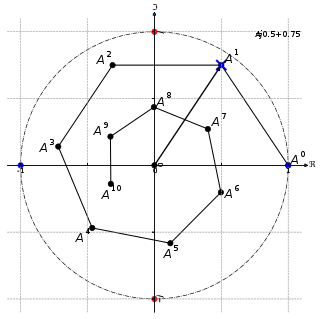
\includegraphics[width=3in]{Exponentials_of_complex_number_within_unit_circle-2.png}
			\begin{tikzpicture}[scale=1.8,>=Stealth]
				% draw axes
				\draw[->, thick, black] (-2,0) -- (2,0) node[below right, black] {$\Re$};
				\draw[->, thick, black] (0,-2) -- (0,2) node[above left, black] {$\Im$};
				
				% draw unit circle
				\draw[blue, thick] (0,0) circle (1.4cm);
				
				% draw point
				\filldraw[red] (1,1) circle (0.08cm) node[anchor=south west, black] {$z = a + ib$};
				
				% draw radius
				\draw[dashed, thick, red] (0,0) -- (1,1) node[midway, above left, black] {$r$};
				
				% draw angle
				\draw[->, thick, orange] (0.3,0) arc (0:45:0.3) node[midway, right, black] {$\theta$};
			\end{tikzpicture}\par
			\vspace{1in}
			{\large Ji Yong-Hyeon\par}
			{\large \today\par}
		\end{center}
	\end{titlepage}
	
	% Table of contents
	\tableofcontents
	
	% Chapters
	\mainmatter
	\iffalse
	\chapter*{Continuity and Derivatives}
	
	\section*{Continuity}
	\begin{tcolorbox}[title=Continuity]
		\begin{definition}
			Let $\varnothing\neq S(\subseteq\R)$. Let $f:S\to\R$ be a real function, and let $\alpha\in S$. We say that \textbf{$f$ is continuous at $\alpha$} if \[
			\forall\varepsilon>0:\exists\delta>0\quad\text{s.t.}\quad\abs{x-\alpha}<\delta\implies\abs{f(x)-f(\alpha)}<\varepsilon.\footnote{$\iff \forall\varepsilon>0:\exists\delta>0\ \text{s.t.}\ f\left(\nbhd_\delta(\alpha)\right)\subseteq\nbhd_\varepsilon\left(f(\alpha)\right)$.}
			\] In other words, \[
			\lim\limits_{x\to\alpha}f(x)=f(\alpha).
			\] If $f$ is continuous on every point of $S$, then $f$ is called a \textbf{continuous function on $S$}.
		\end{definition}
	\end{tcolorbox}
	\begin{remark}
		$f$ is discontinuous at $\alpha$ if and only if \begin{align*}
			&\exists\varepsilon>0\quad\text{s.t.}\quad\forall\delta>0:\abs{x-\alpha}<\delta\ \text{but}\ \abs{f(x)-f(\alpha)}\geq\varepsilon\\
			\iff &\exists\varepsilon>0\quad\text{s.t.}\quad\forall\delta>0:\nbhd_\varepsilon\left(f(\alpha)\right)\subset f\left(\nbhd_\delta(\alpha)\right).
		\end{align*}
	\end{remark}
	
	
	\begin{tcolorbox}[colback=white!10!white,colframe=blue!50!black,title=Continuity]
		A function $f:S(\neq\varnothing)\to\R$ is continuous at $\alpha\in S$ iff \[
		\varepsilon\in\R^+\implies\exists\delta\in\R^+:[f\left[\nbhd_\delta\of{\alpha}\right]\subseteq\nbhd_\varepsilon\of{f\of{\alpha}}].
		\]
	\end{tcolorbox}
	
	\begin{tcolorbox}[colback=red!5!white,colframe=red!75!black,title=Warning]
		This is a warning box. It can be used to alert readers to potential dangers or problems.
	\end{tcolorbox}
	
	\begin{tcolorbox}[colback=white!10!white,colframe=black!50!white,title=Tabular Box,fonttitle=\bfseries\large,sharp corners]
		\begin{tabular}{|c|c|c|}
			\hline
			1 & 2 & 3 \\
			\hline
			4 & 5 & 6 \\
			\hline
			7 & 8 & 9 \\
			\hline
		\end{tabular}
	\end{tcolorbox}
	
	
	The continuity of a function is a fundamental concept that describes the behavior of a function near its domain. A function is said to be continuous at a point $x_0$ in its domain if the limit of the function as $x$ approaches $x_0$ exists and is equal to the function value at $x_0$.
	
	The formal definition of continuity of a function $f(x)$ at a point $x_0$ is:
	
	\begin{align*}
		\lim_{x \to x_0}f(x) &= f(x_0)\
	\end{align*}
	
	That is, the limit of $f(x)$ as $x$ approaches $x_0$ exists and is equal to $f(x_0)$.
	
	If a function is continuous at every point in its domain, then it is said to be a continuous function. There are different types of continuity, such as pointwise continuity, uniform continuity, and local continuity.
	
	Pointwise continuity means that the function is continuous at each point in its domain. Uniform continuity means that the function has a continuous behavior over the entire domain, without any abrupt changes or jumps. Local continuity means that the function is continuous in a small neighborhood around each point in its domain.
	
	The concept of continuity is important in the analysis of functions, and it plays a crucial role in the study of limits, derivatives, and integrals. The continuity of a function also helps us understand its behavior, including the existence of critical points, extreme values, and asymptotic behavior.
	
	In summary, the continuity of a function is a crucial concept in mathematical analysis, and it is essential for understanding the behavior of functions near their domain.
	
	\newpage
	\section{Derivatives}
	\begin{tcolorbox}[title=Differentaible Mapping]
		\begin{definition}
			Let $f:I\to\R$ on an interval $I$ and $\alpha\in I$. A real function $f$ \textbf{is differentiable at the point $\alpha$} if and only if either the limit \[
			f'(\alpha):=\frac{df}{dx}\bigg|_{x=\alpha}:=\mathcolorbox{-blue}{\lim_{x\to\alpha}\frac{f(x)-f(\alpha)}{x-\alpha}}\quad\text{or}\quad \mathcolorbox{-blue}{\lim_{h\to0}\frac{f(\alpha+h)-f(h)}{h}}
			\] exists. Here, $x=\alpha+h$. The real number $f'(\alpha)\in\R$ is the \textbf{derivative of $f$ at the point $\alpha$}.
		\end{definition}
	\end{tcolorbox} 
	\begin{remark}
		A real number $f'(\alpha)\in\R$ is the derivative of $f$ at $\alpha$ if \[
		\varepsilon>0\implies\exists\delta>0: f\left({\nbhd_\delta}^*(\alpha)\right)\subseteq \nbhd_\varepsilon\left(f'(\alpha)\right).
		\]
	\end{remark}
	\
	\begin{tcolorbox}[colback=white]
		\begin{theorem}
			Let $f:I\to\R$ be a real function defined on an interval $I$, and let $\alpha\in I$. \[
			\text{$f$ is differentiable at $\alpha$}\implies\text{$f$ is continuous at $\alpha$}.
			\] In other words, \[
			\exists\lim_{x\to\alpha}\frac{f(\alpha)-f(x)}{x-\alpha}\implies\lim_{x\to\alpha}f(x)=f(\alpha).
			\]
		\end{theorem}
	\end{tcolorbox}
	\begin{proof}
		By hypothesis, $f'(\alpha)$ exists. We have, then, \begin{align*}
			\lim_{x\to\alpha}\left(f(x)-f(\alpha)\right)&=\lim_{x\to\alpha}\left[\frac{f(x)-f(\alpha)}{(x-\alpha)}(x-\alpha)\right]\\
			&=\lim_{x\to\alpha}\frac{f(x)-f(\alpha)}{(x-\alpha)}\cdot\lim_{x\to\alpha}(x-\alpha)\\
			&=f'(\alpha)\cdot0\\
			&=0.
		\end{align*} Hence $\lim\limits_{x\to\alpha}f(x)=f(\alpha)$.
	\end{proof}
	\fi
	
	\chapter{The Complex Number System}
	
	The complex number system is an extension of the real number system that includes a new type of number called the complex number. A complex number is a number that can be expressed in the form $a + bi$, where $a$ and $b$ are real numbers and $i$ is the imaginary unit, which is defined as the square root of $-1$.
	
	The real part of a complex number a + bi is a, and the imaginary part is b. We can represent complex numbers geometrically using the complex plane, which is a two-dimensional plane where the horizontal axis represents the real part of a complex number and the vertical axis represents the imaginary part.
	
	Addition and subtraction of complex numbers are performed by adding or subtracting their real and imaginary parts separately. Multiplication of complex numbers is performed using the distributive property and the fact that $i^2 = -1$. Division of complex numbers is also possible by multiplying both the numerator and denominator by the complex conjugate of the denominator.
	
	The absolute value or modulus of a complex number is the distance between the origin and the point representing the complex number on the complex plane. It is defined as:
	
	\begin{align*}
		|a+bi| &= \sqrt{a^2 + b^2}
	\end{align*}
	
	The argument or phase of a complex number is the angle that the line connecting the origin to the point representing the complex number makes with the positive real axis. It is defined as:
	
	\begin{align*}
		\theta &= \operatorname{arg}(a+bi) = \operatorname{arctan}\left(\frac{b}{a}\right)
	\end{align*}
	
	The complex number system is important in mathematics, physics, engineering, and many other fields. It is used to represent quantities that have both a magnitude and a direction, such as electrical currents and electromagnetic waves. Complex numbers also have applications in signal processing, control theory, and cryptography, among others.
	
	\newpage
	\section{The Field of Complex Numbers}
	
	The set of complex numbers, denoted by $\C$, is defined as the collection of all ordered pairs $(x,y)$ where $x,y\in\R$. The operations of addition and multiplication are defined by:\begin{align*}
		(x_1,y_1)+(x_2+y_2)&=(x_1+x_2,y_1+y_2),\\
		(x_1,y_1)\cdot(x_2+y_2)&=(x_1x_2-y_1y_2,x_1y_2+x_2y_1).
	\end{align*}
	
	We verify that the axioms for a field are met by the definitions given for $\C$: \begin{itemize}
		\item[(F1)] $\of{\C,+}$ is an "Abelian group",
		\item[(F2)] $\of{\C\setminus\set{0},\cdot}$ is an Abelian group, and
		\item[(F3)] the distributive law holds: $x,y,z\in\C\implies\of{x+y}\cdot z=x\cdot z+y\cdot z$.
	\end{itemize}
	
	In (F1), an Abelian group refers to the fact that the operation $+$ on $\C$ satisfies the properties of associativity and commutativity, and \[
	\exists e:=(0,0)\in\C:[(x,y)\in\C\implies(x,y)+e=(x,y)=e+(x,y)].
	\] Additionally, \[
	(x,y)\in\C\implies\exists(-x,-y)\in\C:[(x,y)+(-x,-y)=(0,0)=(-x,-y)+(x,y)].
	\] In condition (F2), the multiplicative identity is (1,0), and the multiplicative inverse of any complex number (x,y) in $\C\setminus\set{(0,0)}$ is determined by \begin{align}
		\of{\frac{x}{x^2+y^2},\frac{-y}{x^2+y^2}}.
	\end{align}
	
	\begin{exercise}
		Verify that (1.1) is indeed the inverse of $(x,y)\in\C\setminus\set{(0,0)}$.
		\begin{proof}[\sol]
			Let $(x,y)\in\C$. Then \begin{align*}
				(x,y)\cdot\of{\frac{x}{x^2+y^2},\frac{-y}{x^2+y^2}}
				&=\of{\frac{x^2}{x^2+y^2}-\frac{-y^2}{x^2+y^2},\frac{-xy}{x^2+y^2}+\frac{xy}{x^2+y^2}}\\
				&=\of{\frac{x^2+y^2}{x^2+y^2},\frac{-xy+xy}{x^2+y^2}}\\
				&=(1,0).
			\end{align*}
		\end{proof}
	\end{exercise}
	
	\begin{tcolorbox}[colback=white,colframe=procolor, title={\color{white}\bf Complex Numbers are Field}]
		\begin{proposition}
			$\of{\C,+,\cdot}$ is a field.
		\end{proposition}
	\end{tcolorbox}
	
	\newpage
	\section{Geometric Representation of Complex Numbers}
	Note that $\C\approx\R^2$ (vector space):
	\begin{center}
		\begin{tikzpicture}[scale=1.5]
			% draw axes
			\draw[->] (-.5,0) -- (1.5,0) node[right] {$\Re(z)$};
			\draw[->] (0,-.5) -- (0,1.5) node[above] {$\Im(z)$};
			% add arrow
			%\draw[->] (0,0) -- (1,1) node[midway, above left] {};
			% draw point
			\filldraw[black] (1,1) circle (2pt) node[anchor=south west] {$(x,y)=x+yi$};
			
			\draw[dotted] (0,1) -- (1,1) node[midway, above left] {};
			\draw[dotted] (1,0) -- (1,1) node[midway, above left] {};
		\end{tikzpicture}
	\end{center}
	\vspace{8pt}
	\subsection{Addition}
	Addition $\leftrightarrow$ Vector Addition:
	\begin{center}
		\begin{tikzpicture}[scale=1.5]
			% draw axes
			\draw[->] (-.5,0) -- (2,0) node[right] {$\Re(z)$};
			\draw[->] (0,-.5) -- (0,2) node[above] {$\Im(z)$};
			% add arrow
			\draw[->] (0,0) -- (.5,1) node[midway, above left] {};
			\draw[->] (0,0) -- (1.5,1.5) node[midway, above left] {};
			\draw[->] (0,0) -- (1,.5) node[midway, above left] {};
			% draw point
			\filldraw[black] (.5,1) circle (1pt) node[anchor=south west] {$z_1$};
			\filldraw[black] (1.5,1.5) circle (1pt) node[anchor=south west] {$z_1+z_2$};
			\filldraw[black] (1,.5) circle (1pt) node[anchor=south west] {$z_2$};
			
			\draw[dotted] (.5,1) -- (1.5,1.5) node[midway, above left] {};
			\draw[dotted] (1,.5) -- (1.5,1.5) node[midway, above left] {};
		\end{tikzpicture}
	\end{center}
	\vspace{8pt}
	\subsection{Polar Coordinate}
	\[
	\begin{cases}
		x=r\cos\theta\\
		y=r\sin\theta
	\end{cases},\quad \begin{cases}
		r=\sqrt{x^2+y^2}\geq 0\\
		\theta\in[0,2\pi).
	\end{cases}0
	\]
	\begin{center}
		\begin{minipage}{.45\textwidth}
			\begin{tikzpicture}[scale=2]
				% draw axes
				\draw[->] (-.5,0) -- (1.5,0) node[right] {$\Re(z)$};
				\draw[->] (0,-.5) -- (0,1.5) node[above] {$\Im(z)$};
				% add arrow
				%\draw[->] (0,0) -- (1,1) node[midway, above left] {};
				% draw point
				\filldraw[black] (1,1) circle (1pt) node[anchor=south west] {$(x,y)=x+yi=z$};
				
				\draw[dotted] (0,1) -- (1,1) node[midway, above left] {};
				\draw[dotted] (1,0) -- (1,1) node[midway, above left] {};
			\end{tikzpicture}
		\end{minipage}
		\begin{minipage}{.45\textwidth}
			\begin{tikzpicture}[scale=2]
				% draw axes
				\draw[->] (-.5,0) -- (1.5,0) node[right] {$\Re(z)$};
				\draw[->] (0,-.5) -- (0,1.5) node[above] {$\Im(z)$};
				% add arrow
				%\draw[->] (0,0) -- (1,1) node[midway, above left] {};
				% draw point
				\filldraw[black] (1,1) circle (1pt) node[anchor=south west] {$re^{i\theta}=r\of{\cos\theta+i\sin\theta}$};
				
				\draw[->] (0,0) -- (1,1) node[midway, above left] {$r$};
				\draw[->, thick, red] (.5,0) arc (0:45:.5) node[midway, right, red] {$\theta$};
				\draw[dotted] (0,1) -- (1,1) node[midway, above left] {};
				\draw[dotted] (1,0) -- (1,1) node[midway, above left] {};
			\end{tikzpicture}
		\end{minipage}
	\end{center} \[
	x+yi=z\iff r\of{\cos\theta+i\sin\theta}=re^{i\theta}.
	\]
	\newpage
	\subsection{Multiplication}
	Let \begin{align*}
		z_1=\of{x_1,y_1}\Leftrightarrow r_1\of{\cos\theta_1+i\sin\theta_1},\\
		z_2=\of{x_2,y_2}\Leftrightarrow r_2\of{\cos\theta_2+i\sin\theta_2}.
	\end{align*} Then \begin{align*}
		z_1z_2&=r_1r_2\of{\cos\theta_1+i\sin\theta_1}\of{\cos\theta_2+i\sin\theta_2}\\
		&=r_1r_2\left[\of{\cos\theta_1\cos\theta_2-\sin\theta_1\sin\theta_2}+i\of{\cos\theta_1\sin\theta_2+\sin\theta_1\cos\theta_2}\right]\\
		&=r_1r_2\left[\cos\of{\theta_1+\theta_2}+i\sin\of{\theta_1+\theta_2}\right]\\
		&=r\of{\cos\theta+\sin\theta}\ \text{with}\ \begin{cases}
			r=r_1r_2\\
			\theta=\theta_1+\theta_2.
		\end{cases}
	\end{align*}
	
	\begin{center}
		\begin{tikzpicture}[scale=2]
			% draw axes
			\draw[->] (-3,0) -- (3,0) node[right] {};
			%\draw[->] (0,-.5) -- (0,1.5) node[above] {$\Im(z)$};
			% add arrow
			%\draw[->] (0,0) -- (1,1) node[midway, above left] {};
			% draw point
			\filldraw[black] (1,1) circle (1pt) node[anchor=south west] {$z_1$};
			\filldraw[black] (.5,1.5) circle (1pt) node[anchor=south west] {$z_2$};
			\filldraw[black] (-1,2) circle (1pt) node[anchor=south west] {$z=z_1z_2$};
			
			\draw[->] (0,0) -- (1,1) node[midway, above left] {$r_1$};
			\draw[->] (0,0) -- (.5,1.5) node[midway, above left] {$r_2$};
			\draw[->] (0,0) -- (-1,2) node[midway, left] {$r=r_1r_2$};
			\draw[->, thick, blue] (.2,0) arc (0:45:.2) node[midway, right, blue] {$\theta_1$};
			\draw[->, thick, blue] (.5,0) arc (0:71:.5) node[midway, right, blue] {$\theta_2$};
			\draw[->, thick, red] (1,0) arc (0:116:1) node[midway, right, red] {$\theta=\theta_1+\theta_2$};
		\end{tikzpicture}
	\end{center}
	\vspace{8pt}
	\subsection{De Movire's Formula}
	\begin{tcolorbox}[colback=white,colframe=procolor, title={\color{white}\bf De Moivre's Formula}]
		\begin{proposition}
			Let $n\in\N$. Then \[
			\of{\cos\theta+i\sin\theta}^n=\cos(n\theta)+\sin(n\theta).
			\]  That is, \[
			n\in\N\implies \mathcolorbox{-blue}{\of{e^{i\theta}}^n=e^{in\theta}}.
			\]
		\end{proposition}
	\end{tcolorbox}
	\newpage
	\begin{remark}[Approximation of $\pi$]
		Let $y=\tan x$ then $\frac{d}{dx}y=\sec^2x=1+\tan^2x=1+y^2$. Since $x=\arctan y$, we have $\frac{d}{dy}x=\frac{1}{1+y^2}$, that is, $\frac{d}{dx}\arctan x=\frac{1}{1+x^2}$. Note that \begin{align*}
			\arctan x =\int\frac{d}{dx}\of{\arctan x}dx=\int\frac{1}{1+x^2}dx
			&=\int\sum_{n=0}^\infty\of{-x^2}^ndx\quad\because\frac{1}{1-r}=\sum_{n=0}^\infty r^n\\
			&=\sum_{n=0}^\infty\int(-1)^nx^{2n}dx\\
			&=\sum_{n=0}^\infty(-1)^n\frac{1}{2n+1}x^{2n+1}\\
			&=x-\frac{1}{3}x^3+\frac{1}{5}x^5-\frac{1}{7}x^7+\cdots.
		\end{align*} Since $\tan\frac{\pi}{4}=1\Leftrightarrow\arctan(1)=\frac{\pi}{4}$, we have \[
		\pi=4\cdot\arctan(1)=4\of{1-\frac{1}{3}+\frac{1}{5}-\frac{1}{7}}+\cdots.
		\]
	\end{remark}
	\vspace{8pt}
	\begin{exercise}
		Show that \[
		\frac{\pi}{4}=\arctan\frac{1}{2}+\arctan\frac{1}{3}.
		\]
		\begin{proof}[\sol]
			Note that $(2+i)(3+i)=6+5i-1=5(1+i)$. \begin{center}
				\begin{tikzpicture}[scale=1.5]
					% draw axes
					\draw[->] (-.5,0) -- (6,0) node[right] {$\Re(z)$};
					\draw[->] (0,-.5) -- (0,6) node[above] {$\Im(z)$};
					% add arrow
					\draw[->] (0,0) -- (2,1) node[midway, above left] {};
					\draw[->] (0,0) -- (3,1) node[midway, above left] {};
					\draw[->] (0,0) -- (5,5) node[midway, above left] {};
					% draw point
					\filldraw[black] (2,1) circle (1.5pt) node[anchor=south] {$2+i$};
					\filldraw[black] (3,1) circle (1.5pt) node[anchor=south west] {$3+i$};
					\filldraw[black] (5,5) circle (1.5pt) node[anchor=south west] {$5(1+i)$};
					
					\draw[->, thick, red] (.7,0) arc (0:26:.7) node[midway, right, black] {$\theta_1=\tan^{-1}(1/2)$};
					\draw[->, thick, red] (2.7,0) arc (0:18:2.7) node[midway, right, black] {$\theta_2=\tan^{-1}(1/3)$};
					\draw[->, thick, red] (4.7,0) arc (0:45:4.7) node[midway, right, black] {$\pi/4=\theta_1+\theta_2$};
					
					\draw[dotted] (2,0) -- (2,1) node[] {};
					\draw[dotted] (0,1) -- (2,1) node[] {};
					\draw[dotted] (3,0) -- (3,1) node[] {};
					\draw[dotted] (0,1) -- (3,1) node[] {};
					\draw[dotted] (5,0) -- (5,5) node[] {};
					\draw[dotted] (0,5) -- (5,5) node[] {};
				\end{tikzpicture}
			\end{center}
		\end{proof}
	\end{exercise}
	\vspace{8pt}
	\subsection{$n$-th roots}
	Note that $\omega$ is a $n$-th root of $z$ if $\omega^n=z$. Let \begin{align*}
		z&=r\of{\cos\theta+i\sin\theta}\ \text{with}\ r\geq 0\ \text{and}\ \theta\in[0,2\pi),\\
		w&=\rho\of{\cos\alpha+i\sin\alpha}\ \text{with}\ \rho\geq 0\ \text{and}\ \alpha\in[0,2\pi).
	\end{align*} Then \[
	\omega^n=z\Rightarrow \rho^n(\cos n\alpha+i\sin n\alpha)=r\of{\cos\theta+i\sin\theta}\Rightarrow\begin{cases}
		\rho^n=r\\
		n\alpha=\theta+2k\pi,\ k\in\Z.
	\end{cases}
	\] Thus, \[
	w=\rho\of{\cos\alpha+i\sin\alpha}=\boxed{\sqrt[n]{r}\left[\cos\of{\frac{\theta}{n}+\frac{2\pi k}{n}}+i\sin\of{\frac{\theta}{n}+\frac{2\pi k}{n}}\right]}.
	\]
	\vspace{8pt}
	\begin{example}
		Find all value of $\omega$ such that $\omega^4=-1$.
		\begin{proof}[\sol]
			Let $\omega=re^{i\theta}$ then $w^4=r^4e^{i4\theta}=-1$, and so $\begin{cases}
				r=1\\
				4\theta=\pi +2\pi\cdot k,\ k\in\Z.
			\end{cases}$ Thus, \[
			\omega_k=\exp\of{i\of{\frac{\pi}{4}+\frac{\pi}{2}\cdot k}},\quad k=0,1,2,3.
			\] That is, \begin{align*}
				w_0=\frac{\sqrt{2}}{2}+\frac{\sqrt{2}}{2}i,\quad w_1=-\frac{\sqrt{2}}{2}+\frac{\sqrt{2}}{2}i,\quad w_2=-\frac{\sqrt{2}}{2}-\frac{\sqrt{2}}{2}i,\quad w_3=\frac{\sqrt{2}}{2}-\frac{\sqrt{2}}{2}i.
			\end{align*}
			\begin{center}
				\begin{tikzpicture}[scale=3]
					% draw axes
					\draw[->] (-1.5,0) -- (1.5,0) node[right] {$\Re(z)$};
					\draw[->] (0,-1.5) -- (0,1.5) node[above] {$\Im(z)$};
					\draw[-, red] (1,0) arc (0:360:1) node[midway, right, black] {};
					% add arrow
					\draw[dotted, line width=0.5mm, red] (0,0) -- ({1/sqrt(2)},{1/sqrt(2)}) node[midway, above left] {};
					\draw[dotted, line width=0.5mm, red] (0,0) -- (-{1/sqrt(2)},{1/sqrt(2)}) node[midway, above left] {};
					\draw[dotted, line width=0.5mm, red] (0,0) -- (-{1/sqrt(2)},-{1/sqrt(2)}) node[midway, above left] {};
					\draw[dotted, line width=0.5mm, red] (0,0) -- ({1/sqrt(2)},-{1/sqrt(2)}) node[midway, above left] {};
					
					\draw[dotted] (-{1/sqrt(2)},{1/sqrt(2)}) -- ({1/sqrt(2)},{1/sqrt(2)}) node[] {};
					\draw[dotted] (-{1/sqrt(2)},{1/sqrt(2)}) -- (-{1/sqrt(2)},-{1/sqrt(2)}) node[] {};
					\draw[dotted] (-{1/sqrt(2)},-{1/sqrt(2)}) -- ({1/sqrt(2)},-{1/sqrt(2)}) node[] {};
					\draw[dotted] ({1/sqrt(2)},-{1/sqrt(2)}) -- ({1/sqrt(2)},{1/sqrt(2)}) node[] {};
					% draw point
					\filldraw[black] (1,0) circle (1.5pt) node[anchor=south west] {$1$};
					\filldraw[black] (0,1) circle (1.5pt) node[anchor=south east] {$i$};
					\filldraw[black] (-1,0) circle (1.5pt) node[anchor=south east] {$-1$};
					\filldraw[black] (0,-1) circle (1.5pt) node[anchor=north east] {$-i$};
					\filldraw[blue] ({1/sqrt(2)},{1/sqrt(2)}) circle (1pt) node[anchor=west, blue] {$\omega_0$};
					\filldraw[blue] (-{1/sqrt(2)},{1/sqrt(2)}) circle (1pt) node[anchor=east, blue] {$\omega_1$};
					\filldraw[blue] (-{1/sqrt(2)},-{1/sqrt(2)}) circle (1pt) node[anchor=east, blue] {$\omega_2$};
					\filldraw[blue] ({1/sqrt(2)},-{1/sqrt(2)}) circle (1pt) node[anchor=west, blue] {$\omega_3$};
					%\filldraw[black] ({1/sqrt(2)},0) circle (1pt) node[anchor=east] {$\sqrt{2}$};
					%\filldraw[black] (0,{1/sqrt(2)}) circle (1pt) node[anchor=north] {$\sqrt{2}i$};
					%\filldraw[black] (-{1/sqrt(2)},0) circle (1pt) node[anchor=west] {$-\sqrt{2}$};
					%\filldraw[black] (0,-{1/sqrt(2)}) circle (1pt) node[anchor=south] {$-\sqrt{2}i$};
					
					\draw[->, thick, red] (.25,0) arc (0:45:.25) node[midway, right, black] {$\frac{\pi}{4}$};
					\draw[->, thick, red] ({sqrt(2)/8},{sqrt(2)/8}) arc (45:135:.25) node[midway, above left, black] {$\frac{\pi}{2}$};
					\draw[->, thick, red] (-{sqrt(2)/8},{sqrt(2)/8}) arc (135:225:.25) node[midway, above 
					left, black] {$\frac{\pi}{2}$};
					\draw[->, thick, red] (-{sqrt(2)/8},-{sqrt(2)/8}) arc (225:315:.25) node[midway, below left, black] {$\frac{\pi}{2}$};
				\end{tikzpicture}
			\end{center}
		\end{proof}
	\end{example}
	
	\newpage
	\subsection{Absolute(Modulus) and Conjugate}
	Let $z=x+iy\in\C$ with $x,y\in\R$. Then \begin{itemize}
		\item (Absolute or Modulus) $\abs{z}=\sqrt{x^2+y^2}$.
		\item (Conjugate) $\conjugate{z}=x-yi$.
	\end{itemize}
	\vspace{8pt}
	\begin{tcolorbox}[colback=white,colframe=procolor, title={\color{white}\bf }]
		\begin{proposition}
			Let $z,z_1,z_2\in\C$. Then\begin{enumerate}
				\item $\abs{z_1z_2}=\abs{z_1}\abs{z_2}$
				\item $\conjugate{\conjugate{z}}=z$
				\item $\boxed{z\conjugate{z}=\abs{z}^2}$
				\item $\begin{cases}
					\Re(z)=\frac{z+\conjugate{z}}{2}\\
					\Im(z)=\frac{z-\conjugate{z}}{2i}.
				\end{cases}$
			\end{enumerate}
		\end{proposition}
	\end{tcolorbox}
	\vspace{8pt}
	\begin{remark}[A polynomial with real coefficient]
		Let \[
		P(z)=\sum_{i=0}^dc_iz^i
		\] with $z\in\C$ and $c_i\in\R$. Then \[
		P(\omega)=0\impliedby P(\conjugate{\omega})=0
		\] for all $\omega\in\Z$.
		\begin{proof}
			\[
			\conjugate{P(w)}=\conjugate{0}\iff\conjugate{\sum_{i=0}^dc_iw^i}=0\iff\sum_{i=0}^dc_i\conjugate{w}^i=0.
			\]
		\end{proof}
	\end{remark}
	
	\newpage
	\section{Topology of $\C$}
	
	\begin{itemize}
		\item $d(z_1,z_2)=\abs{z_1-z_2}=\sqrt{(x_1-x_2)^2-(y_1-y_2)^2}$
		\item $\abs{z_1+z_2}\leq\abs{z_1}+\abs{z_2}$
		\item $\abs{z_1-z_2}\geq\abs{\abs{z_1}-\abs{z_2}}$
	\end{itemize}
	Let $S\subseteq C$.
	\begin{itemize}
		\item Interior Point $z_1$: $\exists\varepsilon>0:D(z_1,\varepsilon)\subseteq S$
		\item Exterior Point $z_2$: $\exists\varepsilon>0:D(z_2,\varepsilon)\cap S=\emptyset$
		\item Boundary Point $z_3$: $\forall\varepsilon>0:D(z_3,\varepsilon)\cap S\neq\emptyset\land D(z_3,\varepsilon)\cap S^C\neq\emptyset$
		\item $U(\subseteq\C)$ is open if, for all $z\in U$, $z$ is an interior point, that is, \[
		z\in U\implies\exists\varepsilon>0:D(z,\varepsilon)\subseteq U.
		\]
		\item $V$ is closed if $V^C$ is open.
		\item $A$ is bounded if $\exists M>0:D(0,M)\supset A$.
		\item $K$ is compact if it is bounded closed.
	\end{itemize}
	
	
	
	\iffalse
	\subsection{Convergence and continuity}
	
	\begin{tcolorbox}[colback=white,colframe=defcolor,arc=5pt,title={\color{white}\bf Limit of Complex function}]
		\begin{definition}
			Let $f: \Omega \subseteq \mathbb{C} \rightarrow \mathbb{C}$ be a complex function and $z_0 \in \mathbb{C}$ be a limit point of $\Omega$. We say that the limit of $f(z)$ as $z$ approaches $z_0$ is $L \in \mathbb{C}$ and write
			\[ \lim_{z \to z_0} f(z) = L \]
			if for every $\epsilon > 0$, there exists a $\delta > 0$ such that for all $z \in \Omega$ with $0 < |z - z_0| < \delta$, we have $|f(z) - L| < \epsilon$.
		\end{definition}
	\end{tcolorbox}
	
	\begin{tcolorbox}[colback=white,colframe=defcolor,arc=5pt,title={\color{white}\bf Continuity of Complex function}]
		\begin{definition}
			Let $f: \Omega \subseteq \mathbb{C} \rightarrow \mathbb{C}$ be a complex function and $z_0 \in \Omega$. We say that $f(z)$ is continuous at $z_0$ if for every $\epsilon > 0$, there exists a $\delta > 0$ such that for all $z \in \Omega$ with $|z - z_0| < \delta$, we have $|f(z) - f(z_0)| < \epsilon$.
			
			Equivalently, $f(z)$ is continuous at $z_0$ if and only if $\lim_{z \to z_0} f(z) = f(z_0)$.
			
			We say that $f(z)$ is continuous on $\Omega$ if $f(z)$ is continuous at every point in $\Omega$.
		\end{definition}
	\end{tcolorbox}
	
	\subsection{Domains}
	\begin{tcolorbox}[title=Path; Curve; Contour;]
		\begin{definition}
			A \textbf{path} (or \textbf{curve}) in $\C$ is a continuous function $\gamma:[a,b]\to\C$.
		\end{definition}
	\end{tcolorbox}
	
	\begin{tcolorbox}[title=Stepwise Path;]
		\begin{definition}
			A \textbf{path} (or \textbf{curve}) in $\C$ is a continuous function $\gamma:[a,b]\to\C$.
		\end{definition}
	\end{tcolorbox}
	
	\begin{tcolorbox}[title=Path-connected;]
		\begin{definition}
			An open set $U\subset\C$ is called \textbf{path-connected} if \begin{align*}
				\forall z_1,z_2\in U:\exists\text{a stepwise path}\ \gamma:[a,b]\to\C\ \text{s.t.}\ \gamma(a)=z_1,\gamma(b)=z_2\ \text{and}\\
				t\in[a,b]\implies\gamma(t)\in U.
			\end{align*}
		\end{definition}
	\end{tcolorbox}
	\fi
	
	\newpage
	\section{Elementary Functions : $\exp, \Log$, etc.}
	\begin{tcolorbox}[colback=white,colframe=magenta,arc=5pt,title={\color{white}\bf Summary}]
		Let $z=x+iy\in\C$ with $x,y\in\R$. \begin{enumerate}[(1)]
			\item The Complex Exponential Function; \[
			e^z=e^{x+iy}:=e^x\of{\cos x+i\sin y}.
			\]
			\item Complex Trigonometric Functions; \begin{itemize}
				\item $\displaystyle\cos z:=\frac{e^{iz}+e^{iz}}{2}$.
				\item $\displaystyle\sin z:=\frac{e^{iz}-e^{iz}}{2i}$.
				\item $\displaystyle\tan z:=\frac{\sin z}{\cos z}$.
			\end{itemize}
			\item Complex Hyperbolic Functions; \begin{itemize}
				\item $\displaystyle\cosh z:=\frac{e^{z}+e^{z}}{2}$.
				\item $\displaystyle\sinh z:=\frac{e^{z}-e^{z}}{2}$.
				\item $\displaystyle\tanh z:=\frac{\sinh z}{\cosh z}$.
			\end{itemize}
			\item Logarithm Functions; \[
			\Log(z)=\ln\abs{z}+i\Arg(z)
			\]
			\item Principal Value; \[
			\pv z^c=\exp(\Log z^c)=\exp\of{c\Log z}.
			\]
		\end{enumerate}
	\end{tcolorbox}
	
	\newpage
	\subsection{The exponential $\exp z$}
	\begin{tcolorbox}[colback=white,colframe=defcolor,arc=5pt,title={\color{white}\bf Complex Exponential}]
		\begin{definition}
			The \textbf{complex exponential function} is defined as
			\begin{equation*}
				\exp{z} =\exp{(x+iy)} \triangleq e^{x}(\cos y + i\sin y),
			\end{equation*}
			where $x,y\in\R$ and $i$ is the imaginary unit, $i^2=-1$.
		\end{definition}
	\end{tcolorbox}
	\begin{remark}
		Recall that Taylor series $e^x=\sum_{n=0}^\infty\frac{1}{n!}x^n$. Note that \begin{align*}
			e^{iy}&=1+iy+\frac{1}{2!}(iy)^2+\frac{1}{3!}(iy)^3+\frac{1}{4!}(iy)^4+\frac{1}{5!}(iy)^5+\cdots\\
			&=\of{1-\frac{1}{2!}y^2+\frac{1}{4!}y^4-\cdots}+i\of{y-\frac{1}{3!}y^3+\frac{1}{5!}y^5-\cdots}\\
			&=\cos y+i\sin y.
		\end{align*} Then $e^{iy}=\cos y+i\sin y$. Thus, we have $
		\exp z=e^x(\cos y+i\sin y)=e^{x+iy}.
		$
	\end{remark}
	
	\begin{tcolorbox}[colback=white,colframe=procolor,arc=5pt,title={\color{white}\bf Properties of Complex Expoenential}]
		\begin{proposition}
			Let $z,z_1,z_2\in\C$. \begin{enumerate}[(1)]
				\item $\exp 0 = 1$.
				\item $\exp\of{z_1+z_2}=(\exp z_1)(\exp z_2)$.
				\item $\exp z\neq 0\implies\inv{\of{\exp z}}=\exp(-z)$.
				\item $\exp(z+2\pi i)=\exp z$.
				\item $\abs{\exp z}=e^{\Re\of{z}}$
			\end{enumerate}
		\end{proposition}
	\end{tcolorbox}
	\begin{proof}
		\begin{itemize}
			\item[(2)] Let $z_1=x_1+iy_1$ and $z_2=x_2+iy_2$. Then \begin{align*}
				\exp\of{z_1+z_2}=\exp\of{x_1+x_2+i(y_1+y_2)}&=e^{x_1+x_2+i(y_1+y_2)}\\
				&=e^{x_1+iy_1}e^{x_2+iy_2}\\
				&=\of{\exp z_1}\of{\exp z_2}.
			\end{align*}
			\item[(3)] $1=\exp 0=\of{\exp z}\of{\exp (-z)}$.
			\item[(4)] $\exp (z+2\pi)=e^z\of{\cos 2\pi+i\sin 2\pi}=\exp z(1+i\cdot 0)=\exp z$.
			\item[(5)] $\abs{\exp\of{z}}=\abs{e^x\cos y+e^x\sin y}=\sqrt{e^{2x}\cos^2y+e^{2x}\sin^2y}=e^x=e^{\Re\of{z}}$.
		\end{itemize}
	\end{proof}
	\newpage
	\begin{remark}[Conformality]
		\ \begin{center}
			\begin{minipage}{.45\textwidth}
				\begin{tikzpicture}[scale=2]
					% draw axes
					\draw[->] (-1.5,0) -- (1.5,0) node[right] {};
					\draw[->] (0,-1.5) -- (0,1.5) node[above] {};
					% add arrow
					\draw[line width=0.5mm, red] (-1.5,.5) -- (1.5,.5) node[below left] {$i\theta_0$};
					\draw[line width=0.5mm, blue] (.5,-1.5) -- (.5,1.5) node[right] {$x_0+iy$};
					\draw[line width=0.5mm, dotted, red] (-1.5,.7) -- (1.5,.7) node[above left] {};
					\draw[line width=0.5mm, dotted, blue] (.3,-1.5) -- (.3,1.5) node[right] {};
					% draw point
					\filldraw[black] (0,0) circle (.5pt) node[below left, black] {$O$};
					\filldraw[blue] (.5,0) circle (1pt) node[right] {$x_0$};
				\end{tikzpicture}
			\end{minipage}$\overset{w=\exp z}{\longrightarrow}$
			\begin{minipage}{.45\textwidth}
				\begin{tikzpicture}[scale=2]
					% draw axes
					\draw[->] (-1.5,0) -- (1.5,0) node[right] {};
					\draw[->] (0,-1.5) -- (0,1.5) node[above] {};
					% add arrow
					%\draw[->] (0,0) -- (1,1) node[midway, above left] {};
					% draw point
					\draw[red] (0,0) circle (1pt) node[below left, black] {$O$};
					%\draw[line width=.5mm, blue] (0,0) circle (30pt) node[above left] {$e^{x_0}$};
					\draw[line width=.5mm, -, blue] (1,0) arc (0:360:1) node[right] {$e^{x_0}$};
					\draw[line width=.5mm, red] (0,0) -- (1.1,1.1) node[midway, above left] {};
					\draw[->, thick, red] (.5,0) arc (0:45:.5) node[midway, right, red] {$\theta$};
					\draw[line width=.5mm, dotted, blue] (0,0) circle (25pt) node[above left] {};
					\draw[line width=.5mm, dotted, red] (0,0) -- (0.35,1.4) node[midway, above left] {};
				\end{tikzpicture}
			\end{minipage}
		\end{center}
	\end{remark}
	\vspace{8pt}
	\subsection{Trigonometric Functions}
	The complex exponential function is intimately connected to trigonometry. The trigonometric functions are defined using the complex exponential function. Let $x\in\R$ then \[
	\exp\of{ix}=\cos x+i\sin x\quad\text{and}\quad\exp\of{-ix}=\cos x-i\sin x.
	\] This gives \[
	\sin(x) = \frac{e^{ix} - e^{-ix}}{2i}\quad\text{and}\quad\cos(x) = \frac{e^{ix} + e^{-ix}}{2}.	
	\] 
	\vspace{8pt}
	\begin{tcolorbox}[colback=white,colframe=defcolor,arc=5pt,title={\color{white}\bf Complex Trigonometric}]
		\begin{definition}
			Let $z\in\C$. Then \begin{align*}
				\cos\of{z}:=\frac{1}{2}\left[\exp(iz)+\exp(-iz)\right],\quad
				\sin\of{z}:=\frac{1}{2i}\left[\exp(iz)-\exp(-iz)\right].
			\end{align*}
		\end{definition}
	\end{tcolorbox}
	\vspace{8pt}
	\begin{tcolorbox}[colback=white,colframe=procolor,arc=5pt,title={\color{white}\bf Properties of Complex Trigonometric}]
		\begin{proposition}
			Let $z,z_1,z_2\in\C$. \begin{enumerate}[(1)]
				\item $\sin\of{\frac{\pi}{2}-z}=\cos z$
				\item $\cos z$ and $\sin z$ are not bounded (by Liouville's Theorem).
				\item $\cos^z+\sin^2z=1$
			\end{enumerate}
		\end{proposition}
	\end{tcolorbox}
	\newpage
	\begin{remark}
		Let $z,z_1,z_2\in\C$. \begin{itemize}
			\item $\begin{cases}
				\sin z=0\Leftrightarrow z=n\pi& (n\in\Z),\\
				\cos z=0\Leftrightarrow z=\of{n+\frac{1}{2}}\pi& (n\in\Z).
			\end{cases}$
			\item $\begin{cases}
				\sin(3z)=3\sin z-4\sin^3z,\\
				\cos(3z)=4\cos^3z-3\cos z.
			\end{cases}$
			\item $\begin{cases}
				\sin^2\frac{z}{2}&=\displaystyle\frac{1-\cos z}{2}\\
				\cos^2\frac{z}{2}&=\displaystyle\frac{1+\cos z}{2}\\
				\tan^2\frac{z}{2}&=\displaystyle\frac{1-\cos z}{1+\cos z}\\
			\end{cases}$
			\item $\begin{cases}
				\cos(z_1+z_2)&=\cos z_1\cos z_2-\sin z_1\sin z_2\\
				\sin(z_1+z_2)&=\sin z_1\cos z_2-\cos z_1\sin z_2\\
				\tan(z_1+z_2)&=\frac{\tan z_1+\tan z_2}{1-\tan z_1\tan z_2}
			\end{cases}$
			\item $\begin{cases}
				\sin(-z)&=-\sin z\\
				\cos(-z)&=\cos z\\
				\tan(-z)&=-\tan z
			\end{cases}$
		\end{itemize}
	\end{remark}
	
	\subsection{Hyperbolic Functions}
	
	\begin{tcolorbox}[colback=white,colframe=defcolor,arc=5pt,title={\color{white}\bf Complex Hyperbolic}]
		\begin{definition}
			Let $z\in\C$. Then \begin{align*}
				\cosh\of{z}:&=\cos(iz)=\frac{1}{2}(e^z+e^{-z}),\\
				\sinh\of{z}:&=\frac{1}{i}\sin(iz)=\frac{1}{2}(e^z-e^{-z}).
			\end{align*}
		\end{definition}
	\end{tcolorbox}
	\vspace{8pt}
	\begin{tcolorbox}[colback=white,colframe=procolor,arc=5pt,title={\color{white}\bf Properties of Complex Hyperbolic}]
		\begin{proposition}
			Let $z,z_1,z_2\in\C$. \begin{enumerate}[(1)]
				\item $\cosh^z-\sinh^2z=1$
				\item $\begin{cases}
					\sinh(z_1+z_2)&=\sinh z_1\cosh z_2+\cosh z_1\sinh z_2,\\
					\cosh(z_1+z_2)&=\cosh z_1\cosh z_2+\sinh z_1\sinh z_2.
				\end{cases}$
				\item $\begin{cases}
					\cosh(-z)&=\cosh(z)\\
					\sinh(-z)&=-\sinh(z)
				\end{cases}$
			\end{enumerate}
		\end{proposition}
	\end{tcolorbox}
	
	\newpage
	\subsection{Logarithm Function}
	
	\begin{tcolorbox}[colback=white,colframe=defcolor,arc=5pt,title={\color{white}\bf Principal Argument}]
		\begin{definition}
			The \textbf{principal argument} of a complex number $z$, denoted by $\operatorname{Arg}(z)$, is defined to be the unique value $\theta \in (-\pi, \pi]$ such that $$
			z=\abs{z}e^{i\theta}=\abs{z}\of{\cos\theta+i\sin\theta}.
			$$
		\end{definition}
	\end{tcolorbox}
	\begin{example}
		\[
		\Arg(1)=0,\quad \Arg(-1)=\pi,\quad\Arg(i)=\frac{\pi}{2},\quad\Arg(-i)=\frac{3}{2}\pi.
		\]
	\end{example}
	\vspace{8pt}
	\begin{tcolorbox}[colback=white,colframe=defcolor,arc=5pt,title={\color{white}\bf Principal Logarithm}]
		\begin{definition}
			The \textbf{principal logarithm} $\Log z$ ($z\neq 0$) is defined by \[
			\Log z = \ln\abs{z}+i\Arg(z).
			\]
		\end{definition}
	\end{tcolorbox}
	\vspace{4pt}
	\begin{remark}
		The principal logarithm satisfies the following properties:
		\begin{itemize}
			\item $\operatorname{Log}(z_1 z_2) = \operatorname{Log}(z_1) + \operatorname{Log}(z_2)$ for all $z_1, z_2 \in \mathbb{C} \setminus (-\infty,0]$.
			\item $\operatorname{Log}(e^z) = z$ for all $z \in \mathbb{C}$.
			\item $\exp(\operatorname{Log}(z)) = z$ for all $z \in \mathbb{C} \setminus (-\infty,0]$.
		\end{itemize}
	\end{remark}
	
	\begin{remark}
		Let $z$ be a non-zero complex number. Then the logarithm of $z$, denoted by $\log z$, is defined to be any complex number $w$ such that $e^w = z$.
		
		However, since $e^{w+2\pi i} = e^w$, there are infinitely many possible values of $\log z$. In fact, the set of all possible values of $\log z$ is given by
		\[ \log z = \ln|z| + i\arg z + 2\pi ik \]
		where $\ln|z|$ is the natural logarithm of the modulus of $z$, $\arg z$ is the argument of $z$, and $k$ is any integer.
		
		Note that the complex logarithm is not continuous on the entire complex plane, since there is a branch cut along the negative real axis. However, it is analytic on any simply connected domain that does not contain the origin.
		
		The principal logarithm of a complex number $z$, denoted by $\operatorname{Log}(z)$, is defined to be the complex number $w = \ln |z| + i \operatorname{Arg}(z)$.
		
		Note that the principal logarithm is a single-valued function defined on the domain $\mathbb{C} \setminus (-\infty,0]$.
	\end{remark}
	
	\newpage
	\chapter{Complex Differentiability}
	
	\section{Complex Differentiability}
	\begin{tcolorbox}[colback=white,colframe=defcolor,arc=5pt,title={\color{white}\bf Complex Differentiability}]
		\begin{definition}
			A complex function $f:U(\subseteq\C)\to\C$, $U$ is an open subset, is said to be \textbf{complex differentiable} at a point $z_0\in U$ if $\exists f'(z_0)$ defined by\[
			f'(z_0)=\frac{df}{dz}\bigg|_{z=z_0}:=\mathcolorbox{-blue}{\lim_{z\to z_0}\frac{f(z)-f(z_0)}{z-z_0}}
			\]
		\end{definition}
	\end{tcolorbox}
	\begin{remark}
		We say that a complex function $f(z)$ is differentiable at a point $z_0\in U$ if \[
		\exists f'\of{z_0}\in\C:\left[\forall\varepsilon>0:\exists\delta>0:\forall z\in U:0<\abs{z-z_0}<\delta\Rightarrow\abs{\frac{f(z)-f(0)}{z-z_0}-f'(z_0)}<\varepsilon\right].
		\] 
	\end{remark}
	\vspace{8pt}
	\begin{example}[\textcolor{red}{$\star\star\star$}]
		\ \begin{enumerate}[(1)]
			\item Let $f\of{z}=z^2$ then \[
			\lim\limits_{\Delta z\to 0}\frac{f(z+\Delta z)-f(z)}{\Delta z}=\lim\limits_{\Delta z\to 0}\frac{z^2+2z\Delta z+(\Delta z)^2-z^2}{\Delta z}=\lim\limits_{\Delta z\to 0}(2z+\Delta z)=2z.
			\]
			\item Let $f\of{z}=\conjugate{z}$ then \[
			\lim\limits_{\Delta z\to 0}\frac{\conjugate{z+\Delta z}-\conjugate{z}}{\Delta z}=\lim\lim_{\Delta z\to 0}\frac{\conjugate{z}+\conjugate{\Delta z}-\conjugate{z}}{\Delta z}=\lim\limits_{\Delta z\to 0}\of{\frac{\conjugate{\Delta z}}{\Delta z}}=\begin{cases}
				1 &\Delta z=\Delta x+i\cdot 0,\\
				-1 &\Delta z= 0+i\cdot\Delta y.
			\end{cases}
			\] Thus $\nexists f'(z)$ for all $z\in\C$.
			\item Let $f\of{z}=\abs{z}^2=z\conjugate{z}$ then\[
			\lim\limits_{\Delta z\to 0}\frac{(z+\Delta z)(\conjugate{z}+\conjugate{\Delta z})-z\conjugate{z}}{\Delta z}=\lim\limits_{\Delta z\to 0}\frac{z\conjugate{\Delta z}+\conjugate{z}\Delta z+\Delta z\conjugate{\Delta z}}{\Delta z}=\lim\limits_{\Delta z\to 0}\of{z\cdot\of{\frac{\conjugate{\Delta z}}{\Delta z}}+\conjugate{z}+\conjugate{\Delta z}}.
			\] Thus $z=0\implies\exists f'(z)$.
		\end{enumerate}
	\end{example}
	
	
	\begin{tcolorbox}[colback=white,colframe=lemcolor,arc=5pt,title={\color{white}\bf Equivalence of Complex Differentiability}]
		\begin{lemma}
			Let $U$ be an open set in $\C$, $z_0\in U$, and  $f:U\to C$. Then  the following are equivalent: \begin{enumerate}[(1)]
				\item $f$ is complex differentiable at $z_0$
				\item There exists an $r>0$, and function $h:D(z_0,r)\to\C$, where $D(z_0,r):=\set{z\in C:\abs{z-z_0}<r}$, such that \begin{itemize}
					\item[(a)] $f\of{z}=f\of{z_0}+[f'(z_0)+h(z)](z-z_0)$ for $\abs{z-z_0}<r$ and 
					\item[(b)] $\lim\limits_{z\to z_0}h\of{z}=0$.
				\end{itemize}
			\end{enumerate}
		\end{lemma}
	\end{tcolorbox}
	\begin{proof}
		\begin{itemize}
			\item[($\Rightarrow$)] Suppose that the complex derivative $f'(z_0)$ exists: \[
			f'(z_0) = \lim_{z \to z_0} \frac{f(z) - f(z_0)}{z - z_0}.
			\] We want to show that there an $r>0$ and a function $h:D\of{z_0,r}$ satisfying condition (a) and (b). Let $\varepsilon>0$. Define the function $h: D(z_0, \delta) \to \mathbb{C}$ by
			\[
			h(z) = \begin{cases}
				\frac{f(z) - f(z_0)}{z - z_0} - f'(z_0) &:z\neq z_0,\\
				0 &:z=z_0.
			\end{cases}
			\] Then \begin{itemize}
				\item[] (Case I) ($z\neq z_0$, \ie, $0<\abs{z-z_0}<\delta$) \begin{align*}
					h(z)=\frac{f(z) - f(z_0)}{z - z_0} - f'(z_0)\overset{\text{Rearraning}}{\implies}f\of{z}=f\of{z_0}+[f'(z_0)+h(z)](z-z_0).
				\end{align*}
				\item[] (Case II) ($z= z_0$, \ie, $0=\abs{z-z_0}$)\[
				f\of{z}=f\of{z_0}+[f'(z_0)+h(z)](z-z_0)\leftrightsquigarrow f\of{z_0}=f\of{z_0}+\crossout[red]{0}{[f'(z_0)+0]\cdot 0}.
				\]
			\end{itemize} Thus, $f\of{z}=f\of{z_0}+[f'(z_0)+h(z)](z-z_0)$ holds whenever $\abs{z-z_0}<\delta$. By the definition of $f'(z_0)$, we have
			\[
			\abs{\frac{f(z)-f(0)}{z-z_0}-f'(z_0)}=\abs{h}=\abs{h(z)-0}<\varepsilon.
			\]
			\item[($\Leftarrow$)] For $z\in D\of{z_0,r}\setminus\set{z_0}$, we have, upon rearranging, that \[
			\frac{f(z)-f(0)}{z-z_0}-f'(z_0)=h(z)\xrightarrow{z\to z_0} 0
			\] and so $\exists f'(z_0)$.
		\end{itemize}
	\end{proof}
	
	
	\begin{tcolorbox}[colframe=procolor, title={\color{white}\bf }]
		\begin{proposition}
			Let $U$ be an open subset of $\C$. Let $f,g:U\to\C$ are complex differentiable at $z_0\in U$. Let $\alpha,\beta\in\C$. \begin{itemize}
				\item (Linearity) \[
				\left(\alpha f\pm\beta g\right)'(z_0)=\alpha f'(z_0)\pm\beta g'(z_0).
				\]
				\item (Product Rule) \[
				\left(fg\right)'(z_0)=f'(z_0)g(z_0)+f(z_0)g'(z_0).
				\]
				\item (Quotient Rule) \[
				\left(\frac{f}{g}\right)'(z_0)=\frac{f'(z_0)g(z_0)-f(z_0)g'(z_0)}{g^2(z_0)}.
				\]
			\end{itemize}
		\end{proposition}
	\end{tcolorbox}
	\vspace{8pt}
	\begin{tcolorbox}[colframe=procolor, title={\color{white}\bf Chain Rule}]
		\begin{proposition}
			Let $f:I_f\to\R$ and $g:I_g\to\R$ satisfies \begin{enumerate}[(i)]
				\item $f(I_f)\subseteq I_g$;
				\item $f$ is differentiable at $x=c$;
				\item $g$ is differentaible at $y=f(c)$.
			\end{enumerate} Define $h:I_f\to\R$ as follows: \[
			h(t)=g(f(t)):=g\circ f(t)
			\] with $t\in I_f$. Then \[
			h'(c)=g'(f(c))f'(c),
			\] \ie, \[
			\mathcolorbox{-blue}{(g\circ f)'(c)=g'(f(c))f'(c)}.
			\]
		\end{proposition}
	\end{tcolorbox}
	
	\newpage
	\section{Cauchy-Riemann Equations}
	
	
	\begin{tcolorbox}[colframe=thmcolor, title={\color{white}\bf Cauchy-Riemann Equations}]
		\begin{theorem}
			Let $U\of{\subseteq\C}$ be an open set, and let \[f:U\to\C:f(z) =f\of{x+yi} = u(x, y) + iv(x, y)
			\] be a complex-valued function, where $u(x, y)$ and $v(x, y)$ are real-valued functions, that is, \begin{align*}
				u:U\to\R&:(x,y)\mapsto \Re\of{f(x+iy)}\quad\text{and}\\ v:U\to\R&:\of{x,y}\mapsto\Im\of{f(x+iy)}.
			\end{align*} If $f(z)$ is differentiable at a point $z_0 = x_0 + iy_0$, then the partial derivatives of $u(x, y)$ and $v(x, y)$ satisfy the Cauchy-Riemann equations: 
			\[
			u_x=v_y\quad\text{and}\quad u_y=-v_x\quad\text{at $(x_0,y_0)$}.
			\]
			%\begin{align*}
			%\frac{\partial u}{\partial x}= \frac{\partial v}{\partial y}\quad\text{and}\quad
			%\frac{\partial u}{\partial y}= -\frac{\partial v}{\partial x}\quad\text{ at $(x_0, y_0)$}.
			%\end{align*}
		\end{theorem}
	\end{tcolorbox}
	
	\begin{proof}
		Let $f'(z_0)$ be the complex derivative of $f(z)$ at $z_0$. By definition, we have \begin{align*}
			f'(z_0)=\lim_{\Delta z\to 0}\frac{f\of{z_0+\Delta z}-f\of{z_0}}{\Delta z}=\begin{cases}
				\displaystyle\lim\limits_{\substack{\Delta x\to 0\\ \Delta y=0}}\frac{f\of{z_0+\Delta z}-f\of{z_0}}{\Delta z} &\cdots\cdots(1)\\
				\displaystyle\lim\limits_{\substack{\Delta y\to 0\\ \Delta x=0}}\frac{f\of{z_0+\Delta z}-f\of{z_0}}{\Delta z}&\cdots\cdots(2).
			\end{cases}
		\end{align*}
		
		\begin{itemize}
			\item[(1)] ($\Delta z=\Delta x+i\cdot 0$);
			\begin{align*}
				(1)&=\lim\limits_{\Delta x\to 0}\frac{\left[u(x_0+\Delta x, y_0)-u\of{x_0,y_0}\right]-i\left[v(x_0+\Delta x,y_0)-v\of{x_0,y_0}\right]}{\Delta x}\\
				&=\frac{\partial u}{\partial x}\of{x_0,y_0}+\frac{\partial v}{\partial x}\of{x_0,y_0}\\
				&= u_x+iv_x\bigg|_{z=z_0}.
			\end{align*}
			\item[(2)] ($\Delta z=0+i\Delta y$);
			\begin{align*}
				(2)&=\lim\limits_{\Delta y\to 0}\frac{\left[u(x_0, y_0+\Delta y)-u\of{x_0,y_0}\right]-i\left[v(x_0,y_0+\Delta y)-v\of{x_0,y_0}\right]}{i\Delta y}\\
				&=\frac{1}{i}\frac{\partial u}{\partial y}\of{x_0,y_0}+\frac{\partial v}{\partial y}\of{x_0,y_0}\\
				&= v_y-iu_y\bigg|_{z=z_0}\quad\text{by multiplying $1=i/i$}.
			\end{align*}
		\end{itemize} Hence we have \[
		(1)=(2)\implies u_x=v_y,\quad u_y=-v_x.
		\]
	\end{proof}
	
	\begin{remark}
		\[\exists f'(z_0):f'(0)=u_x+iv_x\bigg|_{z=z_0}\iff\begin{cases}
			\text{(i)}\ u,v\in C^1\\
			\text{(ii) CR-Eq hold at}\ (x_0,y_0).
		\end{cases}\]
	\end{remark}
	\vspace{8pt}
	\begin{remark}
		Let $z=x+yi$. \begin{table}[h!]
			\centering
			\begin{tabular}{@{}c||cc|cc|cc||cc@{}}
				\toprule
				$f(z)$ & $u(x,y)$ & $v(x,y)$ & $u_x$ & $u_y$ & $v_x$ & $v_y$ & $u_x=v_y$? &$u_y=-v_y$?\\
				\midrule
				$z^2$ & $x^2-y^2$ & $2xy$ & $2x$ & $-2y$ & $2y$ & $2x$ & O & O\\
				\addlinespace
				$\conjugate{z}$ & $x$ & $-y$ & $1$ & $0$ & $0$ & $-1$ & X & X\\
				\addlinespace
				$\abs{z}^2$ & $x^2+y^2$ & $0$ & $2x$ & $2y$ & $0$ & $0$ & if $z=0$ & if $z=0$\\
				\bottomrule
			\end{tabular}
		\end{table}
	\end{remark}
	\vspace{8pt}
	\begin{remark}
		\ \begin{table}[h!]
			\centering
			\begin{tabular}{@{}l||c|c@{}}
				\toprule
				& \textbf{Real Function} & \textbf{Complex Function} \\
				\midrule
				1. Existence of & Sub-seqns & Sub-seqns\\
				limit of sequence & Criterion & Criterion \\
				\hline%\addlinespace
				2. Existence of & Comparison of & Comparison of \\
				limit of function & Left-Right Limit & Approaches \\
				\hline%\addlinespace
				3. Differentiability & Comp. of. LR derivatives & CR-Eqs \\
				\bottomrule
			\end{tabular}
			%\caption{Comparison of real and complex functions}
			%\label{tab:comparison}
		\end{table}
	\end{remark}
	\vspace{8pt}
	\begin{example}
		The function $f:\C\to\C$ is defined by \[
		f\of{z}=\exp z=e^{x+iy}=e^x\of{\cos y+i\sin y}
		\] where $z\in\C$. Then we have \begin{align*}
			u(x,y)&=\Re\of{e^{x+iy}}=e^x\cos y,\\
			v(x,y)&=\Im\of{e^{x+iy}}=e^x\sin y.
		\end{align*} Thus, \begin{align*}
			\frac{\partial u}{\partial x}\of{x,y} &=& e^x\cos y &=& \frac{\partial v}{\partial y}\of{x,y},\\
			\frac{\partial u}{\partial y}\of{x,y} &=& -e^x\sin y &=& -\frac{\partial v}{\partial x}\of{x,y},
		\end{align*} which shows that the Cauchy-Riemann equations hold in $\C$. Since \[
		f'\of{z}=\frac{\partial u}{\partial x}\of{x,y}+i\frac{\partial v}{\partial x}\of{x,y}=e^x\cos y+ie^x\sin y=\exp z,
		\] we also obtain that \[
		\frac{d}{dz}\exp z=\exp z
		\] for $z\in\C$.
	\end{example}
	
	\begin{example}[\textcolor{red}{$\star\star\star$}]
		Consider a complex function $f:D\to\C$. Assume that \begin{enumerate}[(i)]
			\item $f$ is holomorphic in $D$ and
			\item $\abs{f(z)}=c\in\C$, that is, $\abs{f(z)}$ is constant.
		\end{enumerate} Show that $f(z)$ is also constant.
		\begin{proof}
			Let $f=u+iv$ then $\abs{f(z)}=u^2+v^2=c^2$. Note that \[
			\begin{cases}
				2u\cdot u_x+2v\cdot v_x=0\\
				2u\cdot u_y+2v\cdot v_y=0
			\end{cases}\overset{\text{by CR-Eq}}{\implies}\quad\begin{cases}
				2uu_x+2v(-u_y)=0 \cdots\cdots(1)\\
				2uu_y+2vu_x=0 \cdots\cdots(2)
			\end{cases}.
			\] By computing $(1)\cdot u+(2)\cdot v$, we have \[
			2u^2u_x+2v^2u_x=0\implies 2(u^2+v^2)u_x=0\implies 2\cdot c^2\cdot u_x=0.
			\]
			\begin{itemize}
				\item[] (Case 1) $(c=0)$ It is trivial.
				\item[] (Case 2) $(c\neq 0)$ $u_x$ must be $0$.
			\end{itemize} Similarly, we obtain $u_y=0$, and so \[
			u_x=u_y=0,\quad v_x=v_y=0.
			\] That is, $f$ is constant.
		\end{proof}
	\end{example}
	
	\newpage
	\section{Geometric Meaning of the Complex Derivative}
	In $\R$, \[
	\lim\limits_{x\to x_0}\frac{f(x)-f(x_0)}{x-x_0}=f'(x_0)\Rightarrow\frac{f(x)-f(x_0)}{x-x_0}\approx f'(x_0)\ \text{for}\ x\in\mathcal{N}_\delta(x_0)\Rightarrow f(x)-f(x_0)\approx f'(x_0)(x-x_0).
	\]
	In $\C$,
	\[
	\lim\limits_{z\to z_0}\frac{f(z)-f(z_0)}{z-z_0}=f'(z_0)\implies f(z)\approx f(z_0)+f'(z_0)(z-z_0).
	\] Recall that, for $z_1=e^{i\theta_1}$ and $z_2=r_2e^{i\theta_2}$ \[
	\begin{cases}
		z_1z_2=r_1r_2e^{i(\theta_1+\theta_2)}\\
		\arg(z_1z_2)=\arg(z_1)+\arg(z_2).
	\end{cases}
	\] Then \begin{enumerate}
		\item $\arg(f(z)-f(0)\approx\arg\of{f'(z)(z-z_0)}=\arg(f'(z_0))+\arg(z-z_0)$.
		\item $\abs{f(z)-f(z_0)}=\abs{f'(z_0)}\abs{z-z_0}$.
	\end{enumerate}
	\vspace{8pt}
	\section{The d-bar operator}
	\iffalse
	Consider a complex function $f:D\to\C:(x,y)\mapsto f(x,y)$. Let $x=\frac{z+\conjugate{z}}{2}$ and $y=\frac{z-\conjugate{z}}{2i}$. Define a complex function $g$ by \[
	g(z,\conjugate{z}):=f\of{\frac{z+\conjugate{z}}{2},\frac{z-\conjugate{z}}{2}}.
	\]
	\vspace{8pt}
	\begin{example}
		Let $f(z)=\abs{z}^2$ with $\Re(f)=x^2+y^2$ and $\Im(f)=0$. Then \[
		f_x=2x,\quad f_y=2y.
		\] Thus \[
		f(z)=x^2+y^2=\of{\frac{z+\conjugate{z}}{2}}^2+\of{\frac{z-\conjugate{z}}{2i}}^2=z\cdot\conjugate{z}=\abs{z}^2.
		\] Then \[
		\frac{\partial f}{\partial z}=\conjugate{z},\quad
		\frac{\partial f}{\partial \conjugate{z}}={z}.
		\]
	\end{example}
	\vspace{8pt}
	\fi
	\[
	\boxed{\frac{\partial}{\partial z}:=\frac{1}{2}\of{\frac{\partial}{\partial x}-i\frac{\partial}{\partial y}}},\quad\boxed{\frac{\partial}{\partial\conjugate{z}}:=\frac{1}{2}\of{\frac{\partial}{\partial x}+i\frac{\partial}{\partial y}}}.
	\]
	\begin{tcolorbox}[colframe=thmcolor, title={\color{white}\bf }]
		Let $f$ is complex differentiable. Then $\frac{d}{d\conjugate{z}}f=0$.
	\end{tcolorbox}
	\begin{proof}
		\[
		\frac{\partial}{\partial\conjugate{z}}f=\frac{\partial}{\partial\conjugate{z}}u+i\frac{\partial}{\partial\conjugate{z}}v=\frac{1}{2}(u_x+iu_y)+i\frac{1}{2}(u_x+iv_y)=\frac{1}{2}(u_x-v_y)=\frac{1}{2}\of{u_y+v_x}=0.
		\]
	\end{proof}
	\vspace{8pt}
	\begin{example}
		\ \begin{enumerate}
			\item For $f(z)=z^2$, $\frac{\partial}{\partial\conjugate{z}}f=0$
			\item For $f(z)=\conjugate{z}=\frac{\partial}{\partial\conjugate{z}}f=1\neq 0$.
			\item For $f(z)=\abs{z}^2$, $\frac{\partial}{\partial\conjugate{z}}f=z$, \ie, $f$ is differentiable at $z=0$ only. 
		\end{enumerate}
	\end{example}
	
	\newpage
	\chapter{Cauchy Integral Theorem}
	
	\section{Definition of the Contour Integral}
	\begin{tcolorbox}[colback=white,colframe=defcolor,arc=5pt,title={\color{white}\bf Path Integral $\R\to\C$}]
		\begin{definition}
			Define a function $f:[a,b]\to\C:t\mapsto f\of{t}=u\of{t}+iv\of{t}$. Then \[
			\int_a^bf\of{t}dt=\int_a^b\of{u\of{t}+iv\of{t}}dt:=\int_a^bu(t)+i\int_a^bv\of{t}dt.
			\]
		\end{definition}
	\end{tcolorbox}
	\begin{example}
		Compute $\int_0^1\of{t+i}^3dt$.
		\begin{proof}[\sol]
			\begin{itemize}
				\item[(S1)] \begin{align*}
					\int_0^1\of{t+i}^3dt=\int_0^1\of{t^3+3t^2i-3t-i}dt&=\int_0^1\of{t^3-3t}dt+i\int_0^1\of{3t^2-1}dt\\
					&=\frac{1}{4}t^4-\frac{3}{2}t^3\bigg|_0^1+i\left(t^3-t\bigg|_0^1\right)\\
					&=\frac{1}{4}-\frac{3}{2}\\
					&=-\frac{5}{4}.
				\end{align*}
				\item[(S2)] \begin{align*}
					\int_0^1\of{t+i}^3dt=\frac{1}{4}\of{t+i}^4\bigg|_0^1=\frac{1}{4}\of{(1+i)^4-i^4}&=\frac{1}{4}\of{\of{1+4i+6i^2+4i^3+1}-1}\\
					&=\frac{1}{4}\of{1-6}\\
					&=-\frac{5}{4}.
				\end{align*}
			\end{itemize}
		\end{proof}
	\end{example}
	
	\begin{tcolorbox}[colback=white,colframe=defcolor,arc=5pt,title={\color{white}\bf Length of Curve}]
		\begin{definition}
			Let $\gamma$ be a smooth curve such that \[
			\left[a,b\right]\to\C:z\of{t}=x\of{t}+iy\of{t}.
			\] We define a length $L$ of curve $\gamma$ as follows: \[
			L:=\int_\gamma\abs{dz}=\int_a^b\abs{z'\of{t}}dt.
			\]
		\end{definition}
	\end{tcolorbox}
	\begin{remark}
		\begin{align*}
			\int_\gamma\abs{dz}&=\int_a^b\abs{z'\of{t}}dt\\
			&=\int_a^b\sqrt{\of{\frac{dx}{dt}}^2+\of{\frac{dy}{dt}}^2}dt\\
			&=\lim_{n\to\infty}\sum_{k=1}^{n}\sqrt{\of{\frac{\Delta x_k}{\Delta t}}^2+\of{\frac{\Delta y_k}{\Delta t}}^2}\Delta t.
		\end{align*}
	\end{remark}
	\begin{example}
		Consider a circle $\gamma$ with center $z_0$ and radius $R$:
		\begin{center}
			\begin{tikzpicture}[scale=1.8,>=Stealth]
				% draw axes
				%\draw[->, thick, black] (-2,0) -- (2,0) node[below right, black] {$\Re(z)$};
				%\draw[->, thick, black] (0,-2) -- (0,2) node[above left, black] {$\Im(z)$};
				
				% draw unit circle
				\draw[blue, thick] (0,0) circle (1cm) node[above left, blue] {$\gamma$};
				
				% draw point
				\filldraw[red] (0,0) circle (0.08cm) node[below left, black] {$z_0$};
				\filldraw[red] (0.7,0.7) circle (0.08cm) node[anchor=south west, black] {$z$};
				
				% draw radius
				\draw[dashed, thick, red] (0,0) -- (0.7,0.7) node[midway, below right, black] {$R$};
				
				% draw angle
				%\draw[->, thick, orange] (0.3,0) arc (0:45:0.3) node[midway, right, black] {$\theta$};
			\end{tikzpicture}
		\end{center} For $t\in[0,2\pi]$, \[
		z\of{t}=z_0+Re^{it}=z_0+R\cos t+iR\sin t.
		\] Then 
		\begin{align*}
			\int_{\gamma}\abs{dz}=\int_0^{2\pi}\abs{z'\of{t}}dt
			=\int_0^{2\pi}\abs{\frac{d}{dt}\of{z_0+Re^{it}}}dt
			&=\int_0^{2\pi}\abs{Rie^{it}}dt\\
			&=\int_0^{2\pi}\abs{Ri}\abs{e^{it}}dt\\
			&=\int_0^{2\pi}\sqrt{R^2}\sqrt{\cos^2t+\sin^2t}dt\\
			&=\int_0^{2\pi}Rdt\\
			&=Rt\bigg|_0^{2\pi}\\
			&=2\pi R.
		\end{align*}
	\end{example}
	
	
	\begin{tcolorbox}[colback=white,colframe=defcolor,arc=5pt,title={\color{white}\bf Contour Integral}]
		\begin{definition}
			Let $D\of{\subseteq\C}$ be a domain. Given \begin{enumerate}
				\item a continuous function \[
				f:D\to\C:f\of{z}=u(x,y)+iv(x,y)
				\] with $u,v:D\to\R$, and
				\item a smooth path $$\gamma:[a,b]\to D:\gamma\of{t}=x\of{t}+iy\of{t}$$
				with $x,y:[a,b]\to\R$,
			\end{enumerate} 
			we define \begin{align*}
				\int_\gamma f\of{z}dz:&=\int_a^bf\of{\gamma\of{t}}\gamma'\of{t}dt\\
				&=\int_a^b\of{u\of{\gamma\of{t}}+iv\of{\gamma\of{t}}}\cdot\of{x'\of{t}+iy'\of{t}}dt\\
				&=\int_a^b\of{u\of{\gamma\of{t}}\cdot x'\of{t}-v\of{\gamma\of{t}}\cdot y'\of{t}}dt\\
				&\hspace{5mm} +i\int_a^b\of{u\of{\gamma\of{t}}\cdot x'\of{t}+v\of{\gamma\of{t}}\cdot y'\of{t}}dt.
			\end{align*}
		\end{definition}
	\end{tcolorbox}
	\begin{remark}
		For $c_k\in\left[z_{k-1},z_k\right]$,\begin{align*}
			\int_\gamma f\of{z}dz=\lim_{n\to\infty}\sum_{k=1}^nf\of{c_k}\Delta z_k=\lim_{n\to\infty}\sum_{k=1}^nf\of{c_k}\of{\frac{\Delta x}{\Delta t}+i\frac{\Delta y}{\Delta t}}\Delta t
			&=\int_a^bf\of{\gamma\of{t}}\of{x'\of{t}+iy'\of{t}}dt\\
			&=\int_a^bf\of{\gamma\of{t}}\gamma'\of{t}dt.
		\end{align*}
	\end{remark}
	\begin{example}
		Consider a function \[
		f:\C\setminus\set{0}\to\C:f\of{z}=\frac{1}{z}
		\] and two smooth paths
		\begin{align*}
			\gamma_1=\exp\of{it},\quad t\in\left[0,2\pi\right]\\
			\gamma_2=\exp\of{2it},\quad t\in\left[0,\pi\right].
		\end{align*} Then \begin{align*}
			\int_{\gamma_1}f\of{z}dz=\int_{0}^{2\pi}f\of{\exp\of{it}}i\exp\of{it}dt=\int_0^{2\pi}idt=it\bigg|_{0}^{2\pi}=2\pi i,\\
			\int_{\gamma_2}f\of{z}dz=\int_{0}^{\pi}f\of{\exp\of{2it}}2i\exp\of{2it}dt=\int_0^{\pi}2idt=2it\bigg|_{0}^{\pi}=2\pi i.
		\end{align*}
	\end{example}
	
	\begin{tcolorbox}[colback=white,colframe=procolor,arc=5pt,title={\color{white}\bf Equivalent paths give the same integral}]
		\begin{proposition}
			Consider two smooth paths: \[
			\gamma:[a,b]\to\C\quad\text{and}
			\quad\tilde{\gamma}:[c,d]\to\C
			\] such that there is a continuously differentiable function $\varphi:[c,d]\to[a,b]$ such that $a=\varphi\of{c}$, $b=\varphi\of{d}$, and $\tilde{\gamma}\of{t}=\of{\gamma\circ\varphi}\of{t}$ for $t\in[c,d]$. 
			\begin{center}
				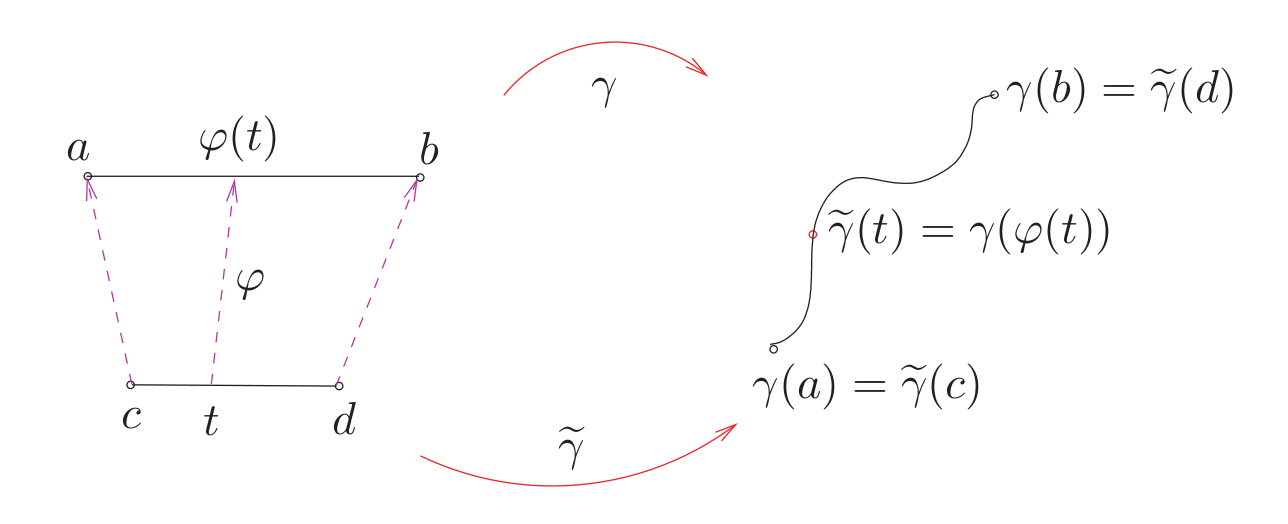
\includegraphics[scale=0.25]{equivalent_paths.png}
			\end{center}
			\begin{align*}
				\int_{\tilde{\gamma}}f\of{z}dz
				&=\int_a^bf\of{\tilde{\gamma}\of{t}}{\tilde{\gamma}'\of{t}}dt \\
				&=\int_a^bf\of{\gamma\of{\varphi\of{t}}}\gamma'\of{\varphi\of{t}}\varphi'\of{t}dt\\
				&=\int_c^df\of{\gamma\of{\tau}}\gamma'\of{\tau}d\tau\quad\text{by $\tau=\varphi\of{t}$}\\
				&=\int_{\gamma}f\of{z}dz.
			\end{align*}
		\end{proposition}
	\end{tcolorbox}
	
	\newpage
	\begin{tcolorbox}[colframe=thmcolor, title={\color{white}\bf An Important Integral}]
		\begin{theorem}
			Let $C$ be a circular path with center $z_0$ and radius $r>0$ traversed in the anti-clockwise direction. Then \[
			\int_C\of{z-z_0}^ndz=\begin{cases}
				2\pi i &:n= -1,\\
				0 &:n\neq -1.
			\end{cases}
			\]
		\end{theorem}
	\end{tcolorbox}
	\begin{proof}
		\begin{itemize}
			\item[(1)] Let $n\neq -1$ then
			\begin{align*}
				\int_C\of{z-z_0}^ndz&=\int_0^{2\pi}\of{z_0+re^{it}-z_0}^n\cdot ire^{it}dt\\
				&=\int_0^{2\pi}r^ne^{i nt}\cdot ire^{it}dt\\
				&=ir^{n+1}\int_0^{2\pi}e^{i(n+1)t}dt\\
				&=ir^{n+1}\left[\frac{1}{i(n+1)}e^{i(n+1)t}\right]_0^{2\pi}\\
				&=0.
			\end{align*}
			\item[(2)] Let $n = -1$ then
			\begin{align*}
				\int_C\of{z-z_0}^{-1}dz=\int_0^{2\pi}\of{re^{it}}^{-1}\cdot ire^{it}dt
				=\int_0^{2\pi}i dt
				=2\pi i.
			\end{align*}
		\end{itemize}
	\end{proof}
	\vspace{4pt}
	\begin{example}
		Consider the following path: \begin{center}
			
			\begin{tikzpicture}[scale=1.1]
				% draw axes
				\draw[->] (-1.5,0) -- (1.5,0) node[right] {$\Re(z)$};
				\draw[->] (0,-1.5) -- (0,1.5) node[above] {$\Im(z)$};
				% add arrow
				%\draw[->] (0,0) -- (1,1) node[midway, above left] {};
				% draw point
				\filldraw[black] (1,1) circle (2pt) node[anchor=south west] {$1+i$};
				\draw[dotted] (0,0) -- (1,1) node[] {};
				
				\draw[line width=0.5mm, ->, thick, red] (0,1) arc (90:360:1) node[midway, left, red] {$C_3$};
				\draw[line width=0.5mm, blue, ->] (1,1) -- (0,1) node[above right] {$C_2$};
				\draw[line width=0.5mm, green, ->] (1,0) -- (1,1) node[midway, right] {$C_1$};
			\end{tikzpicture}
		\end{center} with \begin{align*}
			C_1 &: z_1(t)=1+ti (0\leq t\leq 1)\\
			C_2 &: z_2(t)=(1-t)+i (0\leq t\leq 1)\\
			C_3 &: z_3(t)=e^{it} (\pi/2\leq t\leq 2\pi).
		\end{align*} Let $C=C_1+C_2+C_3$. Find $\int_C\conjugate{z}dz$.
		\begin{proof}[\sol]
			\[
			\int_C\conjugate{z}dz=2i\cdot\of{\text{Area of $C=\partial R$}}=2i\cdot\of{\frac{3\pi}{4}+ 1}=\of{2+\frac{3\pi}{2}}i.
			\]
		\end{proof}
	\end{example}
	
	\newpage
	\section{Properties of Contour Integration}
	
	\begin{tcolorbox}[colback=white,colframe=procolor,arc=5pt,title={\color{white}\bf Linearity of Integration}]
		\begin{proposition}
			Let $D$ be a domain in $\C$ and $\gamma:[a,b]\to D$ be a piecewise smooth path. Then the following hold: for all continuous $f,g:D\to\C$ and all $\alpha\in\C$, \[
			\int_\gamma\left(\alpha f+\beta g\right)\of{z}dz=\alpha\int_\gamma f\of{z}dz+\beta\int_\gamma g\of{z}dz.
			\]
		\end{proposition}
	\end{tcolorbox}
	\vspace{4pt}
	\begin{tcolorbox}[colback=white,colframe=procolor,arc=5pt,title={\color{white}\bf }]
		\begin{proposition}
			Let $\gamma:[a,b]\to D$ be a smooth path in a domain $D$ and $f:D\to\C$ be a continuous function. Then \[
			\int_{-\gamma}f\of{z}dz = -\int_{\gamma}f\of{z}dz.
			\]
		\end{proposition}
	\end{tcolorbox}
	\begin{proof}
		Note that $-\gamma:[a,b]\to\C$ is defined by \[
		\of{-\gamma}\of{t}=\gamma\of{a+b-t}.
		\]\begin{align*}
			\int_{-\gamma}f\of{z}dz &=\int_a^bf\of{\of{-\gamma}\of{t}}\of{-\gamma}'\of{t}dt\\
			&=\int_a^bf\of{\gamma\of{a+b-t}}\frac{d}{dt}\left[\of{-\gamma}\of{t}\right]dt\\
			&=\int_a^bf\of{\gamma\of{a+b-t}}\gamma'\of{a+b-t}\of{-1}dt\\
			&=\int_b^af\of{\gamma\of{\tau}}\gamma'\of{\tau}d\tau\quad\text{by $\tau:=a+b-t$, \ie, $d\tau=-dt$}\\
			&=-\int_a^bf\of{z}dz.
		\end{align*}
	\end{proof}
	\vspace{4pt}
	\begin{tcolorbox}[colback=white,colframe=procolor,arc=5pt,title={\color{white}\bf Concatenation of Paths}]
		\begin{proposition}
			Let $\gamma_1:[a_1,b_1]\to D$ and $\gamma_2:[a_2,b_2]\to D$ be two paths such that $\gamma_1\of{b_1}=\gamma_2\of{a_2}$. Define the concatenation of paths $\gamma_1+\gamma_2:\left[a_1,b_1+b_2-a_2\right]$ as follows: \[
			\of{\gamma_1+\gamma_2}\of{t}=\begin{cases}
				\gamma_1\of{t} &:t\in[a_1,b_1],\\
				\gamma_2\of{t-b_1+a_2} &:t\in[b_1,b_1+b_2-a_2].
			\end{cases}
			\] Then \[
			\int_{\gamma_1+\gamma_2}f\of{z}dz=\int_{\gamma_1}f\of{z}dz+\int_{\gamma_2}f\of{z}dz.
			\]
		\end{proposition}
	\end{tcolorbox}
	\vspace{8pt}
	\begin{tcolorbox}[colback=white,colframe=procolor,arc=5pt,title={\color{white}\bf }]
		\begin{proposition}
			Let \begin{enumerate}
				\item $D$ be a domain in $\C$;
				\item $\gamma:[a,b]\to D$ be a piecewise smooth path and
				\item $f:D\to\C$ be a continuous function.
			\end{enumerate} Then \[
			\abs{\int_\gamma f\of{z}dz}\leq\of{\max_{t\in[a,b]}\abs{f\of{\gamma\of{t}}}}\cdot\int_\gamma\abs{dz}
			\]
		\end{proposition}
	\end{tcolorbox}
	\begin{proof}
		Consider first a curve $\varphi:[a,b]\to\C$. We claim that \[
		\abs{\int_a^b\varphi\of{t}dt}\leq\int_a^b\abs{\varphi\of{t}}dt.
		\] Let $\displaystyle\int_a^b\varphi\of{t}dt=re^{i\theta}$, where $r\geq 0$ and $\theta\in(-\pi,\pi]$. Then \begin{align*}
			\abs{\int_a^b\varphi\of{t}dt}=r
			&=e^{-i\theta}\int_a^b\varphi\of{t}dt\quad\because\int_a^b\varphi\of{t}dt=re^{i\theta}\\
			&=\int_a^be^{-i\theta}\varphi\of{t}dt\\
			&=\int_a^b\Re\of{e^{-i\theta}\varphi\of{t}}dt\quad\because\abs{\int_a^b\varphi\of{t}dt}\in\R\\
			&\leq\int_a^b\abs{\Re\of{e^{-i\theta}\varphi\of{t}}}dt \\
			&\leq\int_a^b\abs{\of{e^{-i\theta}\varphi\of{t}}}dt\quad\because\abs{\Re\of{z}}\leq\abs{z}\\
			&=\int_a^b\abs{\varphi\of{t}}dt\quad\because \abs{e^{-i\theta}}=1.
		\end{align*}
		
		Let $\varphi\of{t}:=f\of{\gamma\of{t}}\cdot\gamma'\of{t}$ with $t\in[a,b]$. Then
		\begin{align*}
			\abs{\int_\gamma f\of{z}dz}&=\abs{\int_a^b f\of{\gamma\of{t}}\gamma'\of{t}dt}\\
			&\leq{\int_a^b \abs{f\of{\gamma\of{t}}\gamma'\of{t}}dt}\\
			&=\int_a^b\abs{f\of{\gamma\of{t}}}\abs{\gamma'\of{t}}dt\\
			&\leq\max_{t\in[a,b]}\abs{f\of{\gamma\of{t}}}\cdot\int_a^b\abs{\gamma'\of{t}}dt.
		\end{align*}
	\end{proof}
	
	\section{Fundamental Theorem of Contour Integration}
	
	\begin{tcolorbox}[colback=white,colframe=thmcolor,arc=5pt,title={\color{white}\bf Fundamental Theorem of Contour Integration}]
		\begin{theorem}
			Let \begin{enumerate}[(i)]
				\item $D$ be a domain in $\C$;
				\item $\gamma:[a,b]\to D$ be a piecewise smooth path;
				\item $f:D\to\C$ be a continuous in $D$;
				\item $F:D\to\C$ be a holomorphic function such that $F'=f$ in $D$.
			\end{enumerate} Then \[
			\int_\gamma f\of{z}dz=F\of{\gamma\of{b}}-F\of{\gamma\of{a}}.
			\]
		\end{theorem}
	\end{tcolorbox}
	\begin{proof}
		For $z=x+iy\in D$, where $x,y\in\R$, we define the real-valued functions $U,V,u,v$ by \begin{align*}
			F(x+iy)&=U(x,y)+iV(x,y),\\
			f(x+iy)&=u(x,y)+iv(x,y).
		\end{align*} Also, set $\gamma\of{t}=x\of{t}+iy\of{t}$ ($t\in[a,b]$). Then
		\begin{align*}
			\int_\gamma f\of{z}dz&=\int_a^bf\of{\gamma\of{t}}\gamma'\of{t}dt\\
			&=\int_a^b\of{u+iv}\of{x'+iy'}dt\\
			&=\int_a^b\of{ux'-vy'}dt +i\int_a^b\of{vx'+uy'}dt\\
			&=\int_a^b\of{U_xx'-V_xy'}dt +i\int_a^b\of{V_xx'+U_xy'}dt\quad\because F'=U_x+iV_x=f=u+iv\\
			&=\int_a^b\of{U_xx'+U_yy'}dt +i\int_a^b\of{V_xx'+V_yy'}dt\quad\text{by CR-Eqs: $U_x=V_y$, $U_y=-V_x$}\\
			&=\int_a^b\frac{d}{dt}\left[U(x,y)\right]dt+i\int_a^b\frac{d}{dt}\left[V(x,y)\right]dt\\
			&=U\of{x(b),y(b)}-U\of{x(a),y(a)}+i\of{V\of{x(b),y(b)}-V\of{x(a),y(a)}}\\
			&=\of{U\of{x(b),y(b)}+U\of{x(a),y(a)}}-\of{V\of{x(b),y(b)}+V\of{x(a),y(a)}}\\
			&=F\of{\gamma\of{b}}-F\of{\gamma\of{a}}.
		\end{align*}
	\end{proof}
	
	
	\newpage
	\section{The Cauchy Integral Theorem}
	
	\begin{tcolorbox}[colback=white,colframe=defcolor,arc=5pt,title={\color{white}\bf Path Homotopy}]
		\begin{definition}
			Consider two closed paths $\gamma_0,\gamma_1:[0,1]\to D$. $\gamma_0$ is \textit{$D$-homotopic to} $\gamma_1$ if there exists a continuous function $H:[0,1]^2\to D$ such that \begin{enumerate}[(H1)]
				\item $\forall t\in[0,1]: H(t,0)=\gamma_0(t)$;
				\item $\forall t\in[0,1]: H(t,1)=\gamma_1(t)$;
				\item $\forall s\in[0,1]: H(0,s)=H(1,s)$.
			\end{enumerate}
		\end{definition}
	\end{tcolorbox}
	\vspace{8pt}
	\begin{example}
		Consider \begin{align*}
			\gamma_0&:[0,1]\to\C:\gamma_0(t)=4e^{2\pi it},\\
			\gamma_1&:[0,1]\to\C:\gamma_1(t)=2i+e^{2\pi it}.
		\end{align*}\begin{center}
			\begin{tikzpicture}[scale=1]
				% draw axes
				\draw[->] (-5,0) -- (5,0) node[right] {$\Re(z)$};
				\draw[->] (0,-5) -- (0,5) node[above] {$\Im(z)$};
				% add arrow
				%\draw[->] (0,0) -- (1,1) node[midway, above left] {};
				% draw point
				\filldraw[blue] (4,0) circle (2pt) node[anchor=south west, black] {$4$};
				\filldraw[blue] (1,2) circle (2pt) node[anchor=south west] {};
				\filldraw[blue] (1.5,1.7) circle (2pt) node[anchor=south west] {};
				\filldraw[black] (0,2) circle (2pt) node[anchor=south west] {$2i$};
				
				\draw[line width=0.5mm, -, thick, black] (4,0) arc (0:360:4) node[midway, above right] {$\gamma_0$};
				\draw[line width=0.5mm, -, thick, black] (1,2) arc (0:360:1) node[above right] {$\gamma_1$};
				\draw[line width=0.5mm, -, thick, red] (1.5,1.7) arc (0:360:1.5) node[midway, left, red] {};
				\draw[line width=0.5mm, -, thick, blue] (4,0) -- (1,2) node[] {};
				%\draw[line width=0.5mm, green, ->] (1,0) -- (1,1) node[midway, right] {$C_1$};
			\end{tikzpicture}
		\end{center} Then $\gamma_0$ is $\C$-homotopic to $\gamma_1$ by \[
		H(t,s)=(1-s)\gamma_0(t)+s\gamma_1(t).
		\] $\gamma_0$ is not $\C\setminus\set{0}$-homotopic to $\gamma_1$.
	\end{example}	
	\vspace{8pt}
	
	\newpage
	\begin{tcolorbox}[colback=white,colframe=thmcolor,arc=5pt,title={\color{white}\bf The Cauchy Integral Theorem}]
		\begin{theorem}
			Let \begin{enumerate}
				\item[(i)] $D$ be a domain in $\C$;\quad (ii) $f:D\to\C$ be holomorphic in $D$, and
				\item[(iii)] $\gamma_0,\gamma_1:[0,1]\to\C$ be two closed, piecewise smooth, $D$-homotopic paths.
			\end{enumerate} Then \[
			\int_{\gamma_0}f\of{z}dz=\int_{\gamma_1}f\of{z}dz.
			\]
		\end{theorem}
	\end{tcolorbox}
	\begin{proof}
		Consider a path homotopy $H:[0,1]^2\to D$ s.t. $H\in C^2$. Let $\gamma_s:=H\of{\cdot, s}$ be a closed path with fixed point $s$. Define \[
		I\of{s}:=\int_{\gamma_s}f\of{z}dz,\quad s\in[0,1].
		\] We must show that $I(0)=I(1)$. Note that \[
		\left[\forall s\in[0,1]:\frac{d}{ds}\left[I(s)\right]=0\right]\implies I(0)=I(1).
		\] We claim that $\displaystyle\frac{d}{ds}\left[I(s)\right]=0$ for $s\in[0,1]$:
		\begin{align*}
			\frac{d}{ds}\left[I(s)\right]&=\frac{d}{ds}\left[\int_{\gamma_s}f\of{z}dz\right]=\frac{d}{ds}\left[\int_0^1f\of{\gamma_s\of{t}}\gamma_s'\of{t}dt\right]\\
			&=\frac{d}{ds}\left[\int_0^1f\of{H\of{t,s}}H_t\of{t,s}dt\right]\\
			&=\int_0^1\frac{\partial}{\partial s}\left[f\of{H\of{t,s}}\frac{\partial}{\partial t}H\of{t,s}\right]dt\\
			&=\int_0^1\left(f'\of{H(t,s)}\cdot \frac{\partial}{\partial s}H\of{t,s}\cdot \frac{\partial}{\partial t}H\of{t,s}+f\of{H(t,s)}\cdot \frac{\partial^2}{\partial s\partial t}H\of{t,s}\right)dt\\
			&=\int_0^1\frac{\partial}{\partial t}\left[f\of{H(t,s)}\frac{\partial }{\partial s}H\of{t,s}\right]dt\quad\because H\in C^2\\
			&=\left[f\of{H(t,s)}\frac{\partial }{\partial s}H\of{t,s}\right]_0^1\\
			&=f\of{H\of{1,s}}\frac{\partial}{\partial s}H\of{1,s}-f\of{H\of{0,s}}\frac{\partial}{\partial s}H\of{0,s}\\
			&=0,
		\end{align*} since \begin{enumerate}[(i)]
			\item By (H3), $H\of{1,s}=H\of{0,s}$ holds.
			\item $\displaystyle\frac{\partial}{\partial s}H\of{1,s}=\lim_{h\to 0}\frac{H\of{1,s+h}-H\of{1,s}}{h}=\lim_{h\to 0}\frac{H\of{0,s+h}-H\of{0,s}}{h}=\frac{\partial}{\partial s}H\of{0,s}$.
		\end{enumerate}
		Hence \[
		\frac{d}{ds}\left[I\of{s}\right]=0\implies I\of{0}=I\of{1}\implies
		\int_{\gamma_0}f\of{z}dz=\int_{\gamma_1}f\of{z}dz.
		\]
	\end{proof}
	\vspace{8pt}
	\begin{tcolorbox}[colback=white,colframe=thmcolor,arc=5pt,title={\color{white}\bf Cauchy-Goursat Theorem}]
		\begin{theorem}
			Let $f:D\to\C$ be a holomorphic function, where $D\subseteq\C$ is a simply connected domain. Let $C$ be a closed contour in $D$. Then \[
			\oint_C f\of{z}dz = 0.
			\]
		\end{theorem}
	\end{tcolorbox}
	
	\begin{remark}[Simply Connected Domain]
		\ \begin{center}
			\begin{tikzpicture}[scale=1.5]
				
				% Connected and simply connected
				\filldraw[fill=green!20] (0,0) ellipse (1cm and 0.5cm);
				\draw (0.8,0) node {$D$};
				\draw (0,-1) node {Connected (\textcolor{blue}{O})};
				\draw (0,-1.4) node {Simply connected (\textcolor{blue}{O})};
				
				% Non-connected and simply connected
				\filldraw[fill=green!20] (4.5,0) circle (0.4cm);
				\draw (4.5,0) node {$D_1$};
				\filldraw[fill=green!20] (3.5,0) circle (0.4cm);
				\draw (3.5,0) node {$D_2$};
				\draw (4,-1) node {Connected (\textcolor{red}{X})};
				\draw (4,-1.4) node {Simply connected (\textcolor{blue}{O})};
				
				% Connected and non simply connected
				\filldraw[fill=green!20] (0,-3) ellipse (1cm and 0.7cm);
				\draw (0.8,-3) node {$D$};
				\draw (0,-4) node {Connected (\textcolor{blue}{O})};
				\draw (0,-4.4) node {Simply connected (\textcolor{red}{X})};
				\filldraw[fill=white] (0,-3) circle (0.2cm);
				
				% Non-connected and non simply connected
				\filldraw[fill=green!20] (4.8,-3) circle (0.6cm);
				\draw (4.8,-3) node {$D_1$};
				\filldraw[fill=green!20] (3.2,-3) circle (0.6cm);
				\filldraw[fill=white] (3.2,-3) circle (0.1cm);
				\draw (3.5,-3) node {$D_2$};
				\draw (4,-4) node {Connected (\textcolor{red}{X})};
				\draw (4,-4.4) node {Simply connected (\textcolor{red}{X})};
				
			\end{tikzpicture}
		\end{center}
	\end{remark}
	\newpage
	\section{Existence of Primitive}
	
	
	\begin{tcolorbox}[colback=white,colframe=thmcolor,arc=5pt,title={\color{white}\bf Anti-derivative Theorem}]
		\begin{theorem}
			Let \begin{enumerate}[(i)]
				\item $D$ is a simply connected domain and
				\item $f:D\to\C$ is holomorphic.
			\end{enumerate} Then there is a holomorphic function $F:D\to\C$ such that \[
			z\in D\implies F'\of{z}=f\of{z}.
			\]
		\end{theorem}
	\end{tcolorbox}
	\begin{proof}
		Fixed a point $p\in D$. Define a function $F:D\to\C$ as follows: \[
		F\of{z}=\int_{\gamma_z}f\of{\zeta}d\zeta
		\] where $\gamma_z$ is a path joining $p$ to $z$. \begin{enumerate}[(i)]
			\item ($F$ is well-defined) Clearly, $\gamma:=\gamma_z+\of{-\tilde{\gamma_z}}$ is closed. Then
			\begin{align*}
				\int_{\gamma}f\of{\zeta}d\zeta=0&\implies \int_{\gamma_z+\of{-\tilde{\gamma_z}}}f\of{\zeta}d\zeta=0\\
				&\implies\int_{\gamma}f\of{\zeta}d\zeta=\int_{\tilde{\gamma_z}}f\of{\zeta}d\zeta
			\end{align*} That is, Cauchy Integral Theorem gives $F$ is well-defined.
			\item (Holomorphicity of $F$ and $F'=f$ in $D$) Since $f$ is holomorphic in $D$, it is also continuous there. Let $\varepsilon>0$. Then \[
			\exists\delta>0:\forall z\in D:\abs{w-z}<\delta\implies\abs{f\of{w}-f\of{z}}<\varepsilon.
			\] We take a $w$ such that $0<\abs{w-z}<\delta$. Then \[
			\frac{F\of{w}-F\of{z}}{w-z}=\frac{1}{w-z}\of{\int_{\gamma_w}f\of{\zeta}d\zeta-\int_{\gamma_z}f\of{\zeta}d\zeta}.
			\] Let $\gamma_{zw}$ is a straight line path joining $z$ to $w$. By the Cauchy Integral Theorem, we obtain \[
			0=\int_{\gamma_z+\gamma_{zw}-\gamma_w}f\of{\zeta}d\zeta\implies\int_{\gamma_{zw}}f\of{\zeta}d\zeta=\int_{\gamma_w}f\of{\zeta}d\zeta-\int_{\gamma_z}f\of{\zeta}d\zeta.
			\] Note that \[
			w-z=\zeta\bigg|_z^w=\int_{\gamma_{zw}}\frac{d}{d\zeta}\left[\zeta\right] d\zeta=\int_{\gamma_{zw}}1d\zeta.
			\]Then \begin{align*}
				\frac{F\of{w}-F\of{z}}{w-z}-f\of{z}&=\frac{1}{w-z}\int_{\gamma_{zw}}f\of{\zeta}d\zeta-f\of{z}\\
				&=\frac{1}{w-z}\int_{\gamma_{zw}}f\of{\zeta}d\zeta-f\of{z}\cdot\frac{1}{w-z}\int_{\gamma_{zw}}1d\zeta\\
				&=\frac{1}{w-z}\int_{\gamma_{zw}}\of{f\of{\zeta}-f\of{z}}d\zeta,
			\end{align*} and so \begin{align*}
				\abs{\frac{F\of{w}-F\of{z}}{w-z}-f\of{z}}&=\abs{\frac{1}{w-z}\int_{\gamma_{zw}}\of{f\of{\zeta}-f\of{z}}d\zeta}\\
				&=\frac{1}{\abs{w-z}}\abs{\int_{\gamma_{zw}}\of{f\of{\zeta}-f\of{z}}d\zeta}\\
				&\leq\frac{1}{\abs{w-z}}\cdot\max_{\zeta\in\gamma_{zw}}\abs{f\of{\zeta}-f\of{z}}\cdot\int_{\gamma_{zw}}\abs{dz}\\
				&<\frac{1}{\abs{w-z}}\cdot\varepsilon\cdot\abs{w-z}\\
				&=\varepsilon.
			\end{align*} Thus $F'\of{z}=f\of{z}$, and $F$ is holomorphic.
		\end{enumerate}
	\end{proof}
	
	\newpage
	\section{The Cauchy Integral Formula}
	\begin{tcolorbox}[colback=white,colframe=procolor,arc=5pt,title={\color{white}\bf }]
		\begin{proposition}
			Let \begin{enumerate}[(1)]
				\item $D$ be a domain;
				\item $f:D\to\C$ be holomorphic in $D\setminus\set{0}$, and continuous on $D$;
				\item the disc $\Delta:=\set{z\in\C:\abs{z-z_0}\leq r}\subset D$ with $r>0$ and $z_0\in D$.
			\end{enumerate} Then \[
			f\of{z_0}=\frac{1}{2\pi i}\int_{C_r}\frac{f\of{z}}{z-z_0}dz,\quad \abs{z-z_0}<r,
			\] where $C_r$ is the circular path $C_r\of{t}=z_0+re^{it}$, $t\in[0,2\pi]$, with enter $z_0$ and radius $r>0$ traversed in the anti-clockwise direction.
		\end{proposition}
	\end{tcolorbox}
	\begin{proof}
		Let $\varepsilon>0$. We must show that \[
		\abs{\frac{1}{2\pi i}\int_{C_r}\frac{f\of{z}}{z-z_0}dz-f\of{z_0}}<\varepsilon.
		\] The continuity of $f$ on $D$ gives \[
		\exists\delta:\abs{z-z_0}<\varepsilon\implies\abs{f\of{z}-f\of{z_0}}<\varepsilon.
		\] Since $C_r$ is $D\setminus\set{z_0}$-homotopic to $C_\delta$, we have \[
		\int_{C_r}\frac{f\of{z}}{z-z_0}dz=\int_{C_\delta}\frac{f\of{z}}{z-z_0}dz
		\] Note that \[
		\int\frac{1}{z-z_0}dz=2\pi i.
		\] Thus, \begin{align*}
			\abs{\frac{1}{2\pi i}\int_{C_r}\frac{f\of{z}}{z-z_0}dz-f\of{z_0}}&=
			\abs{\frac{1}{2\pi i}\int_{C_\delta}\frac{f\of{z}}{z-z_0}dz-f\of{z_0}}\\
			&=\abs{\frac{1}{2\pi i}\int_{C_\delta}\frac{f\of{z}}{z-z_0}dz-\frac{1}{2\pi i}\cdot f\of{z_0}\cdot\int_{C_\delta}\frac{1}{z-z_0}dz}\\
			&=\abs{\frac{1}{2\pi i}\int_{C_\delta}\frac{f\of{z}-f\of{z_0}}{z-z_0}dz}\\
			&\leq\frac{1}{\abs{2\pi i}}\cdot\max_{\substack{z\in C_\delta\\ (\abs{z-z_0}=\delta)}}\abs{\frac{f\of{z}-f\of{z_0}}{z-z_0}}\cdot\int_{C_\delta}\abs{dz}\\
			&<\frac{1}{2\pi}\cdot\frac{\varepsilon}{\delta}\cdot 2\pi\delta\\
			&=\varepsilon.
		\end{align*}
	\end{proof}
	
	\begin{tcolorbox}[colback=white,colframe=thmcolor,arc=5pt,title={\color{white}\bf The Cauchy Integral Formula for Circular Paths}]
		\begin{theorem}
			Let \begin{enumerate}[(1)]
				\item $D$ be a domain;
				\item $f:D\to\C$ be holomorphic in $D$ and $z_0\in D$;
				\item the disc $\Delta:=\set{z\in\C:\abs{z-z_0}\leq r}\subset D$ with $r>0$ and $z_0\in D$.
			\end{enumerate} Then \[
			f\of{w}=\frac{1}{2\pi i}\int_{C_r}\frac{f\of{z}}{z-w}dz,\quad \abs{w-z_0}<r,
			\] where $C_r$ is the circular path $C_r\of{t}=z_0+re^{it}$, $t\in[0,2\pi]$, with enter $z_0$ and radius $r>0$ traversed in the anti-clockwise direction.
		\end{theorem}
	\end{tcolorbox}
	\begin{proof}
		Since $\displaystyle\frac{f\of{z}}{z-w
		}$ is holomorphic in $D\setminus\set{w}$ and $C_\delta$ is $D\setminus\set{w}$-homotopic to $C_{r}$,
		\begin{align*}
			f\of{w}=\frac{1}{2\pi i}\int_{C_\delta}\frac{f\of{z}}{z-w}dz=\frac{1}{2\pi i}\int_{C_r}\frac{f\of{z}}{z-w}dz.
		\end{align*}
	\end{proof}
	
	\begin{tcolorbox}[colback=white,colframe=corcolor,arc=5pt,title={\color{white}\bf The Cauchy Integral Formula for General Paths}]
		\begin{corollary}
			Let \begin{enumerate}[(1)]
				\item $D$ be a domain;
				\item $f:D\to\C$ be holomorphic in $D$;
				\item $\gamma$ be a closed path in $D$ which is $D\setminus\set{z_0}$-homotopic to a circular path $C$ centered at $z_0$, such that $C$ and its interior is contained in $D$.
			\end{enumerate} Then $\displaystyle f\of{z_0}=\frac{1}{2\pi i}\int_\gamma\frac{f\of{z}}{z-z_0}dz$.
		\end{corollary}
	\end{tcolorbox}
	
	\newpage
	\section{Holomorphic Functions are Infinitely Differentiable}
	\begin{tcolorbox}[colback=white,colframe=corcolor,arc=5pt,title={\color{white}\bf }]
		\begin{corollary}
			Let \begin{enumerate}[(1)]
				\item $D$ be a domain;
				\item $f:D\to\C$ be holomorphic in $D$;
			\end{enumerate} Then $f'$ is holomorphic in $D$.
		\end{corollary}
	\end{tcolorbox}
	\begin{remark}
		The above gives the following chain of implications: \[
		\boxed{f\in\Hol\of{D}}\Rightarrow\boxed{f'\in\Hol\of{D}}\Rightarrow\boxed{f''\in\Hol\of{D}}\Rightarrow\cdots\boxed{f^{\of{n}}\in\Hol\of{D}}\Rightarrow\cdots.
		\]
	\end{remark}
	\begin{proof}
		(Naive Proof) Let $\displaystyle f\of{z}=\frac{1}{2\pi i}\int_\gamma\frac{f\of{\zeta}}{\zeta-z}d\zeta$. Then \begin{align*}
			f'\of{z}&=\frac{1}{2\pi i}\frac{d}{dz}\left[\int_\gamma\frac{f\of{\zeta}}{\zeta-z}d\zeta\right]\\
			&=\frac{1}{2\pi i}\int_\gamma\frac{d}{dz}\left[\frac{f\of{\zeta}}{\zeta-z}\right]d\zeta\quad\text{(an assumption)}\\
			&=\frac{1}{2\pi i}\int_\gamma\frac{f\of{\zeta}}{\of{\zeta-z}^2}d\zeta,
		\end{align*} and $f''\of{z}=\displaystyle\frac{1}{2\pi i}\cdot 2\int_\gamma\frac{f\of{\zeta}}{\of{\zeta-z}^3}d\zeta$. Thus \[
		f^{\of{n}}\of{z}=\frac{n!}{2\pi i}\int_\gamma\frac{f\of{\zeta}}{\of{\zeta-z}^{n+1}}d\zeta.
		\]
	\end{proof}
	
	\newpage
	\section{Liouville's Theorem; F.T.A.}
	\begin{tcolorbox}[colback=white,colframe=thmcolor,arc=5pt,title={\color{white}\bf Liouville's Theorem}]
		\begin{theorem}
			Every bounded entire function is constant.
		\end{theorem}
	\end{tcolorbox}
	\begin{proof}
		Let $M\geq 0$ be such that $\forall z\in\C:\abs{f\of{z}}\leq M$. Choose $w\in\C$, and let \[
		\gamma\of{t}=w+Re^{it},\quad t\in[0,2\pi].
		\] By generalized Cauchy integral theorem, \[
		f'\of{w}=\frac{1}{2\pi i}\int_\gamma\frac{f\of{z}}{\of{z-w}^2}dz,
		\] and so \begin{align*}
			\abs{f'\of{w}}=\abs{\frac{1}{2\pi i}\int_\gamma\frac{f\of{z}}{\of{z-w}^2}dz}&\leq\abs{\frac{1}{2\pi i}}\cdot\max_{z\in\gamma}\abs{\frac{f\of{z}}{\of{z-w}^2}}\cdot\int_\gamma\abs{dz}\\
			&\leq\frac{1}{2\pi}\cdot\frac{M}{R^2}\cdot 2\pi R\\
			&=\frac{M}{R}.
		\end{align*} Since $R>0$ was arbitrary, it follows that $f'\of{w}=0$, and hence $f$ is constant.
	\end{proof}
	
	\begin{tcolorbox}[colback=white,colframe=corcolor,arc=5pt,title={\color{white}\bf Fundamental Theorem of Algebra}]
		\begin{corollary}
			Every polynomial of degree $\geq 1$ has a root in $\C$.
		\end{corollary}
	\end{tcolorbox}
	\begin{proof}
		Let $P:\C\to\C:P\of{z}=\sum_{i=1}^d c_iz^i=c_0+c_1z+\cdots+c_dz^d$ is a polynomial with $d\geq 1$. Suppose that $P(z)$ has no root in $\C$, that is, for all $z\in\C$, $P\of{z}\neq 0$. Define the function $f$ by $f\of{z}=1/P\of{z}$ ($z\in\C$), is entire. Note that \[
		\abs{z}>R\implies\exists M,R>0:\abs{P\of{z}}\geq M\abs{z}^d.
		\] And so \[
		\abs{P\of{z}}\leq\max\set{\frac{1}{MR^d},\frac{1}{m}},\quad z\in\C.
		\] By Liouville's Theorem, $f$ must be constant, and so $P$ must be a constant, a contradiction to the fact that $d\geq 1$.
	\end{proof}
	
	\newpage
	\section{Morera's Theorem}
	\begin{tcolorbox}[colback=white,colframe=thmcolor,arc=5pt,title={\color{white}\bf Morera's Theorem}]
		\begin{theorem}
			Let \begin{enumerate}[(i)]
				\item $D$ is a domain;
				\item $f:D\to\C$ is a continuous function such that
				\item for every closed path $\gamma$ in every disc contained in $D$, $\oint_\gamma f\of{z}dz=0$.
			\end{enumerate} Then $f$ is holomorphic in $D$.
		\end{theorem}
	\end{tcolorbox}
	\begin{proof}
		Let $z_0\in D$. Consider $z\in D$ with $z\neq z_0$. For two distinct path $\gamma_1,\gamma_2$ joining $z_0$ to $z$, define $\gamma:=\gamma_1+\of{-\gamma_2}$. Then \begin{align*}
			&\oint_\gamma f\of{\zeta}d\zeta=\int_{\gamma_1}f\of{\zeta}d\zeta-\int_{\gamma_2}f\of{\zeta}d\zeta=0\\
			\implies&\int_{\gamma_1}f\of{\zeta}d\zeta=\int_{\gamma_2}f\of{\zeta}d\zeta.
		\end{align*} We define \[
		F\of{z}:=\int_{z_0}^zf\of{\zeta}d\zeta.
		\] Then $F'\of{z}=f\of{z}$ and $F\in\Hol$, and so $F^{(n)}\in\Hol$. Thus, $\exists F''\of{z}$ and then $F''\of{z}=f'\of{z}$. Hence $f$ is holomorphic in $D$.
	\end{proof}
	
	\newpage
	\section{Special Content}
	\subsection{Line Integral of Real function}
	
	\begin{align*}
		\int_C\textbf{F}\cdot d\textbf{r}:&=\int_a^b\textbf{F}\of{x(t),y(t)}\cdot\of{x'(t),y'(t)}dt\\
		&=\int_a^bP\of{x(t),y(t)}\frac{dx(t)}{dt}dt+\int_a^bQ\of{x(t),y(t)}\frac{dy(t)}{dt}dt\\
		&=\int_C Pdx+Qdy.
	\end{align*}
	\vspace{4pt}
	\begin{example}
		Let $\textbf{F}(x,y)=\of{-y,x}$, and let $C\of{t}=\of{a\cos t,b\sin t}$ for $t\in[0,2\pi]$. Then \[
		\oint_C\textbf{F}\cdot d\textbf{r}=\int_0^{2\pi}\of{-b\sin t, a\cos t}\cdot\of{-a\sin t, b\cos t}dt=\int_0^{2\pi}ab dt=2\pi ab.
		\]
	\end{example}
	\vspace{8pt}
	\subsection{Green's Theorem}
	Let $C=\partial R$ be a simple close contour (counter-clockwise). Consider two functions $P,Q:D\to\R$ with $P,Q\in C^1$. Then \[
	\int_{C=\partial R} Pdx+Qdy=\iint_R\of{\frac{\partial Q}{\partial x}-\frac{\partial P}{\partial y}}dxdy.
	\]
	\vspace{8pt}
	\subsection{Fundamental Theorem of Calculus (Generalized ver.)}
	\[
	\boxed{\int_{\partial R}f=\iint_R df}
	\]
	\vspace{4pt}
	\begin{remark}
		Let $f:=Pdx+Qdy$ then \begin{align*}
			df=d\of{Pdx+Qdy}&=(dPdx+Pd(dx))+(dQdy+Qd(dy))\\
			&=dPdx+dQdy\quad\because d(dx)=0=d(dy)\\
			&=\of{P_xdx+P_ydy}dx+\of{Q_xdx+Q_ydy}dy\\
			&=P_ydydx+Q_xdxdy\quad\because dxdx=0=dydy\\
			&=\of{Q_x-P_y}dxdy\quad\because dxdy=-dydx.
		\end{align*}
	\end{remark}
	\vspace{4pt}
	\begin{example}
		\[
		\int_{C=\partial R}\of{x^2+y^2}dx+\of{2xy}dy=\iint_R\left[\frac{\partial}{\partial x}2xy-\frac{\partial}{\partial y}\of{x^2+y^2}\right]dxdy=\iint_R\of{2y-2y}dxdy=0.
		\]
	\end{example}
	
	\newpage
	\begin{remark}[Area]
		Area($C$)$:=\displaystyle\frac{1}{2}\oint_{C=\partial R}xdy-ydx$.
		\begin{proof}
			\[
			\oint_{C=\partial R}xdy-ydx=\iint_R\of{\frac{\partial}{\partial x}x-\frac{\partial}{\partial y}(-y)}dxdy=2\iint_Rdxdy=2\cdot \text{Area($C$)}.
			\]
		\end{proof}
	\end{remark}
	\vspace{4pt}
	\begin{example}
		Let $C\of{t}=\of{a\cos t, b\sin t}$ for $t\in[0,2\pi]$ then \[
		\oint_Cxdy-ydx=\int_0^{2\pi}a\cos t\cdot b\cos t dt-\int_0^{2\pi}b\sin t\cdot (-a)\sin t dt=\int_0^{2\pi}abdt=2\pi ab.
		\] Thus the area is $S=\pi ab$.
	\end{example}
	\vspace{4pt}
	\begin{example}
		Let $C(t)=a\cos t+ib\sin t$ for $t\in[0,2\pi]$. Then \begin{align*}
			\int_C\conjugate{z}dz&=\int_0^{2\pi}\of{x(t)-iy(t)}\of{x'(t)+iy'(t)}dt\\
			&=\int_0^{2\pi}\of{xx'+yy'}dt+i\int_0^{2\pi}\of{-yx'+xy'}dt\\
			&=\oint_Cxdx+ydy+i\oint_C\of{-y}dx+xdy\\
			&=\iint_R\of{\frac{\partial}{\partial x}y-\frac{\partial}{\partial y}x}dxdy+i\iint_R\of{\frac{\partial}{\partial x}x-\frac{\partial}{\partial y}\of{-y}}dxdy\\
			&=0+i2\iint_Rdxdy\\
			&=2i\cdot\text{Area($C$)}.
		\end{align*}
		Thus, \[
		\text{Area($C$)}=\frac{1}{2i}\int_C\conjugate{z}dz.
		\]
	\end{example}
	
	\subsection{Cauchy-Goursat Theorem for Multiply-connected Domain}
	Let $f$ is holomorphic in simply counter-clockwise connected contours $C$,$C_1$ and $C_2$. Then \[
	\int_Cf\of{z}dz=\int_{C_1}f\of{z}dz+\int_{C_2}f\of{z}dz.
	\]
	\begin{proof}
		Let $\tilde{C}:=C-C_1-C_2$. By Cauchy-Goursat Theorem, \[
		\int_{\tilde{C}}f\of{z}dz=0,
		\] and so \[
		\int_Cf\of{z}dz=\int_{C_1}f\of{z}dz+\int_{C_2}f\of{z}dz.
		\]
	\end{proof}
	
	\begin{exercise}
		Find \[
		\frac{1}{2\pi i}\oint_C\frac{e^{\alpha z}}{z^2+1}dz
		\] with $C\of{t}=3e^{it}$ for $t\in[0,2\pi]$.
		\begin{center}
			\begin{tikzpicture}[scale=1.25]
				\begin{axis}[
					xmin=-4, xmax=4,
					ymin=-4, ymax=4,
					axis lines=center,
					xlabel={$\Re$},
					ylabel={$\Im$},
					xlabel style={anchor=west},
					ylabel style={anchor=south},
					xtick={-3,3},
					ytick={-1,1},
					grid=major,
					domain=0:2*pi,
					samples=100,
					variable=\t,
					legend pos=outer north east,
					]
					
					% Contour C(t) = 3e^{it}
					\addplot[smooth, color=blue, thick] ({3*cos(deg(\t))}, {3*sin(deg(\t))});
					\addlegendentry{$C(t) = 3e^{it}$}
					
					% Poles at i and -i
					\node[circle, draw, red, fill=red, inner sep=1pt, label=right:$i$] at (axis cs:0,1) {};
					\node[circle, draw, red, fill=red, inner sep=1pt, label=right:$-i$] at (axis cs:0,-1) {};
				\end{axis}
			\end{tikzpicture}
		\end{center}
		
		\begin{proof}[\sol]
			Note that \[
			\frac{1}{z^2+1}=\frac{1}{\of{z+i}\of{z-i}}=\frac{1}{2i}\of{\frac{1}{z-i}-\frac{1}{z+i}}.
			\] Let $f(z)=e^{\alpha z}$ then \begin{align*}
				\frac{1}{2\pi i}\oint_C\frac{e^{\alpha z}}{z^2+1}dz&=\frac{1}{2\pi i}\oint_C\frac{f\of{z}}{2i}\of{\frac{1}{z-i}-\frac{1}{z+i}}dz\\
				&=\frac{1}{2\pi i}\frac{1}{2i}\oint_C\of{\frac{f\of{z}}{z-i}-\frac{f\of{z}}{z+i}}dz\\
				&=\frac{1}{2i}\left[\frac{1}{2\pi i}\int_C\frac{f\of{z}}{z-i}dz-\frac{1}{2\pi i}\int_C\frac{f\of{z}}{z+i}dz\right]\\
				&=\frac{1}{2i}\of{f\of{i}-f\of{-i}}\quad\text{by Cauchy Integral formula}\\
				&=\frac{e^{\alpha i}-e^{-\alpha i}}{2i}\\
				&=\sin\alpha.
			\end{align*}
		\end{proof}
	\end{exercise}
	
	
	\newpage
	\chapter{Taylor and Laurent series}
	
	\iffalse
	\begin{tikzpicture}[x=0.75pt,y=0.75pt,yscale=-1,xscale=1]
		%uncomment if require: \path (0,300); %set diagram left start at 0, and has height of 300
		
		%Shape: Polygon Curved [id:ds09006776322026155] 
		\draw   (251.33,82) .. controls (271.33,72) and (424,45.33) .. (444,111.33) .. controls (464,177.33) and (446.67,199.33) .. (402.67,224) .. controls (358.67,248.67) and (252.67,242) .. (232.67,212) .. controls (212.67,182) and (231.33,92) .. (251.33,82) -- cycle ;
		
	\end{tikzpicture}
	\fi
	
	\begin{note}[Convergence of Sequence]
		\[
		\lim\limits_{n\to\infty}a_n=A\overset{\text{def.}}{\iff}\forall\varepsilon>0:\exists N\in\N:\left[n\geq N\implies\abs{a_n-A}<\varepsilon\right].
		\]
	\end{note}
	
	\section{Series}
	Let $\set{a_n}$ is a sequence in $\C$. The sequence $\set{s_k}$ defined by \begin{align*}
		s_1 &:= a_1 \\
		s_2 &:= a_1+a_2 \\
		&\vdots\\
		s_k&:=a_1+a_2+\cdots+a_{k-1}+a_k\\
		&\vdots
	\end{align*} The numbers $s_k$ are called the \textbf{partial sums}.
	\vspace{8pt}
	\begin{tcolorbox}[colback=white,colframe=defcolor,arc=5pt,title={\color{white}\bf Convergence of Series}]
		\begin{definition}
			\ \begin{enumerate}[(1)]
				\item The series $\sum_{n=1}^\infty a_n$ \textbf{converges} if $\sum_{n=1}^\infty a_n:=\lim\limits_{n\to\infty}s_n=\lim\limits_{n\to\infty}\of{\sum_{k=1}^na_k}$.
				\item The series $\sum_{n=1}^\infty a_n$ \textbf{diverges} if $\set{s_n}_{n\in\N}$ is diverges.
				\item The series $\sum_{n=1}^\infty a_n$ \textbf{converges absolutely} if the real series $\sum_{n=1}^\infty\abs{a_n}$ converges.
			\end{enumerate}
		\end{definition}
	\end{tcolorbox}
	\vspace{8pt}
	\begin{note}
		Let $\set{a_n}_{n\in\N}$ is positive bounded. Then \[
		\sum a_n\ \text{converges}\iff\exists M\in\C:\left[n\in\N\implies\sum_{k=1}^\infty\leq M\right].
		\]
	\end{note}
	\vspace{4pt}
	\begin{note}[\textbf{Integral Test}]
		Let $f:[1,\infty)\to\mathbb{R}^+$ be a decreasing function on $[1,\infty)$. Then the series $\sum_{k=1}^\infty f(k)$ converges if and only if the improper integral \[
		\int_{1}^\infty f(x)\ dx = \lim\limits_{b\to\infty}\int_{1}^bf(x)\ dx
		\] exists. In the case of convergence, the partial sum $S_n=\sum_{k=1}^nf(k)$ and the sum $S=\sum_{k=1}^\infty f(k)$ satisfy the estimate \[
		\int_{n+1}^\infty f(x)\ dx\leq S-S_n\leq\int_{n}^\infty f(x)\ dx.
		\]
		\begin{center}
			\begin{tikzpicture}[scale=2]
				% Axes
				\draw[->] (0,0) -- (6.5,0) node[right] {$x$};
				\draw[->] (0,0) -- (0,2) node[above] {$y$};
				
				% Function curve
				\draw[domain=.5:6.5,smooth,variable=\x,blue] plot ({\x},{1/(\x)}) node[above] {$f(x)=\frac{1}{x}$};
				
				% Rectangles
				\foreach \n in {1,...,5} {
					\draw[pattern=north east lines, pattern color=red] (\n,0) rectangle (\n+1,{1/(\n)});
				}
				
				% Labels
				\foreach \n in {1,...,5} {
					\node[below] at (\n,0) {\n};
				}
				\node[below] at (5.5,0) {$\cdots$};
				\node[left] at (0,1) {1};
				\node[below left] at (0,0) {0};
				
				% Series and integral
				\node[anchor=west, text width=6cm] at (4,1.7) {Series: $\displaystyle\sum_{n=1}^{\infty} \frac{1}{n}$};
				\node[anchor=west, text width=6cm] at (4,1) {Integral: $\displaystyle\int_1^{\infty} \frac{1}{x} \, dx$};
			\end{tikzpicture}
		\end{center}
	\end{note}
	\vspace{4pt}
	\begin{example}[$p$-series]
		The $p$-series \[
		\sum_{n=1}^\infty\frac{1}{n^p}=1+\frac{1}{2^p}+\frac{1}{3^p}+\cdots
		\] converges when $p>1$ and diverges when $p\leq 1$.
	\end{example}
	\vspace{8pt}
	\begin{note}[Ratio Test]
		Let $\sum a_n$ be a series such that \[
		r=\lim\limits_{n\to\infty}\abs{\frac{a_{n+1}}{a_n}}.
		\]\begin{enumerate}
			\item If $r<1$ then the series $\sum a_n$ is absolutely convergent.
			\item If $r>1$ then the series $\sum a_n$ is divergent.
			\item If $r=1$ then this test gives no information.
		\end{enumerate}
	\end{note}
	\vspace{4pt}
	\begin{example}
		Determine whether $\sum_{n=1}^\infty\frac{n^n}{n!}$ converges.
		\begin{proof}[\sol]
			Let $a_n=\frac{n^n}{n!}$ then \[
			\frac{a_{n+1}}{a_n}=\frac{\frac{\of{n+1}^{n+1}}{\of{n+1}!}}{\frac{n^n}{n!}}=\frac{(n+1)(n+1)^n}{(n+1)n!}\cdot\frac{n!}{n^n}=\of{\frac{n+1}{n}}^n=\of{1+\frac{1}{n}}^n.
			\] Thus, $\lim\limits_{n\to\infty}\frac{a_{n+1}}{a_n}=\lim\limits_{n\to\infty}\of{1+\frac{1}{n}}^n=e>1$, and so $\sum_{n=1}^\infty\frac{n^n}{n!}$ diverges.
		\end{proof}
	\end{example}
	\vspace{8pt}
	\begin{note}[Root Test]
		Let $\sum a_n$ be a series such that \[
		r=\lim\limits_{n\to\infty}\abs{a_n}^{\frac{1}{n}}.
		\]\begin{enumerate}
			\item If $r<1$ then the series $\sum a_n$ is absolutely convergent.
			\item If $r>1$ then the series $\sum a_n$ is divergent.
			\item If $r=1$ then this test gives no information.
		\end{enumerate}
	\end{note}
	\vspace{4pt}
	\begin{example}
		Determine whether $\sum_{n=2}^\infty\frac{1}{\of{\ln n}^n}$ converges.
		\begin{proof}[\sol]
			Since \[
			\lim\limits_{n\to\infty}\frac{1}{\sqrt[n]{\of{\ln n}^n}}=\lim\limits_{n\to\infty}\frac{1}{\ln n}=0<1,
			\] $\sum_{n=2}^\infty\frac{1}{\of{\ln n}^n}$ converges.
		\end{proof}
	\end{example}
	
	
	\section{Power Series}
	\begin{center}
		\begin{tikzpicture}[scale=.5]
			% Draw circles for sets
			\draw (0,0) circle (1.2cm);
			\draw (0,0) circle (2.2cm);
			\draw (0,0) circle (3cm);
			
			% Labels
			\node[align=center] at (0,0) {\tiny Polynomial};
			\node[align=center] at (0,1.55) {\tiny Power Series};
			\node[align=center] at (0,2.6) {\tiny Series};
			\node[below] at (0,-3) {Polynomial $\subseteq$ Power Series $\subseteq$ Series};
		\end{tikzpicture}
	\end{center}
	\begin{tcolorbox}[colback=white,colframe=defcolor,arc=5pt,title={\color{white}\bf Power Seires}]
		Let $\set{c_n}_{n\in\N}$ be a complex sequence (thought of as a sequence of coefficients). An expression of the type \[
		\sum_{n=0}^\infty c_nz^n
		\] is called a \textbf{power series} in the complex variable $z$.
	\end{tcolorbox}
	\vspace{8pt}
	\begin{tcolorbox}[colback=white,colframe=thmcolor,arc=5pt,title={\color{white}\bf Existence of Radius of Convergence}]
		\begin{theorem}
			For $\sum_{n=0}^\infty c_nz^n$, exactly one of the following hold: \begin{enumerate}[(1)]
				\item Either it is absolutely convergence for all $z\in\C$.
				\item Or there is a unique non-negative real number $R$ (\textbf{radius of convergence}) such that \begin{enumerate}[(a)]
					\item $\sum_{n=0}^\infty c_nz^n$ is absolutely convergent for all $z\in\C$ with $\abs{z}<R$, and
					\item $\sum_{n=0}^\infty c_nz^n$ is divergent for all $z\in\C$ with $\abs{z}>R$.
				\end{enumerate}
			\end{enumerate} If the power series converges for all $z\in\C$, we
			say that the power series has an infinite radius of convergence, and write $R=\infty$.
			
			\begin{center}
				\begin{tikzpicture}[scale=.5]
					% Draw circles for sets
					\draw (0,0) circle (3cm);
					% draw point and radius
					\draw[-] (0,0) -- (3,0) node[midway, above left] {$R$};
					\draw[black] (0,0) circle (2pt) node[left] {$z_0$};
					% Labels
					\node[align=center, blue] at (-1,-1) {converge};
					\node[align=center, red] at (3,3) {diverge};
				\end{tikzpicture}
			\end{center}
		\end{theorem}
	\end{tcolorbox}
	\vspace{8pt}
	\begin{tcolorbox}[colback=white,colframe=thmcolor,arc=5pt,title={\color{white}\bf }]
		\begin{theorem}
			Consider the power series $\sum_{n=0}^\infty c_nz^n$. Let $R$ is the radius of convergence, and let $L:=\lim\limits_{n\to\infty}\abs{\frac{c_{n+1}}{c_n}}$ exists. Then \begin{enumerate}[(1)]
				\item $L\neq 0\implies R=1/L$.
				\item $L=0\implies R=\infty$.
			\end{enumerate}
		\end{theorem}
	\end{tcolorbox}
	\vspace{8pt}
	\begin{tcolorbox}[colback=white,colframe=thmcolor,arc=5pt,title={\color{white}\bf }]
		\begin{theorem}
			Let $f(z):=\sum_{n=0}^\infty c_nz^n$ converges for $\abs{z}<R(>0)$. Then \[
			f'(z)=\sum_{n=1}^\infty nc_nz^{n-1}\quad\text{ for $\abs{z}<R$.}
			\]
		\end{theorem}
	\end{tcolorbox}
	\vspace{4pt}
	\begin{tcolorbox}[colback=white,colframe=corcolor,arc=5pt,title={\color{white}\bf }]
		\begin{corollary}
			Let $f(z):=\sum_{n=0}^\infty c_nz^n$ converges for $\abs{z}<R(>0)$. Then for $k\geq 1$, \[
			f^{(k)}(z)=\sum_{n=k}^\infty\left[\of{\prod_{i=0}^{k-1}(n-i)}c_nz^{n-k}\right]\quad\text{ for $\abs{z}<R$.}
			\] In particular, for $n\geq 0$, $c_n=\displaystyle\frac{1}{n!}f^{(n)}(0)$.
		\end{corollary}
	\end{tcolorbox}
	\vspace{4pt}
	\begin{tcolorbox}[colback=white,colframe=corcolor,arc=5pt,title={\color{white}\bf }]
		\begin{corollary}
			Let $z_0\in\C$, and let $f(z):=\sum_{n=0}^\infty c_n\of{z-z_0}^n$ converges for $\abs{z-z_0}<R(>0)$. Then for $k>1$, \[
			f^{(k)}(z)=\sum_{n=k}^\infty\left[\of{\prod_{i=0}^{k-1}(n-i)}c_n\of{z-z_0}^{n-k}\right]\quad\text{ for $\abs{z-z_0}<R$.}
			\] In particular, for $n\geq 0$, $c_n=\displaystyle\frac{1}{n!}f^{(n)}(z_0)$.
		\end{corollary}
	\end{tcolorbox}
	
	\newpage
	\section{Taylor Series}
	
	\begin{tcolorbox}[colback=white,colframe=thmcolor,arc=5pt,title={\color{white}\bf }]
		\begin{theorem}
			Let $f$ is holomorphic in $D(z_0,R):=\set{z\in\C:\abs{z-z_0}<R}$. Then \[
			f(z)=\sum_{n=0}^\infty c_n\of{z-z_0}^n=c_0+c_1\of{z-z_0}+c_2\of{z-z_0}^2+\cdots
			\] for $z\in D\of{z_0,R}$, where for $n\geq 0$, \[
			c_n=\frac{1}{2\pi i}\oint_C\frac{f\of{\zeta}}{\of{\zeta-z_0}^{n+1}}d\zeta,
			\] and $C$ is the circular path with center $z_0$ and radius $r$, where $0<r<R$ traversed in the anti-clockwise direction.
			\begin{center}
				\begin{tikzpicture}[scale=.7]
					%circle
					\draw[dashed] (3,0) arc (0:360:3) node[midway, right, black] {};
					\draw[-, blue] ({sqrt(2)},{sqrt(2)}) arc (45:360:2) node[above right, black] {};
					\draw[->, blue] (2,0) arc (0:45:2) node[above, black] {$C$};
					
					% add arrow
					\draw[cyan] (0,0) -- (2,0) node[midway, above] {$r$};
					\draw[red] (0,0) -- ({3*1/sqrt(2)},-{3*1/sqrt(2)}) node[midway, above right] {$R$};
					% draw point
					\draw[black] (0,0) circle (1.5pt) node[anchor=east] {$z_0$};
				\end{tikzpicture}
			\end{center}
		\end{theorem}
	\end{tcolorbox}
	\begin{proof}
		Let $z\in D(z_0,R)$. Initially, let $r$ be such that $\abs{z-z_0}<r<R$. Then by Cauchy's Integral Formula, \begin{align*}
			f(z)=\frac{1}{2\pi i}\oint_C\frac{f\of{\zeta}}{\zeta-z}\ d\zeta&=\frac{1}{2\pi i}\oint_C\frac{f\of{\zeta}}{\zeta-z_0+z_0-z}\ d\zeta\\
			&=\frac{1}{2\pi i}\oint_C\frac{f\of{\zeta}}{\of{\zeta-z_0}\of{\displaystyle 1-\frac{z-z_0}{\zeta-z_0}}}\ d\zeta\\
			&=\frac{1}{2\pi i}\oint_C\left[\frac{f\of{\zeta}}{\of{\zeta-z_0}}\cdot\frac{1}{\displaystyle 1-\frac{z-z_0}{\zeta-z_0}}\right]\ d\zeta.
		\end{align*} Set $w:=\displaystyle\frac{z-z_0}{\zeta-z_0}$ then $\abs{w}=\displaystyle\frac{\abs{z-z_0}}{r}<1$. Thus \begin{align*}
			\frac{1}{\displaystyle 1-\frac{z-z_0}{\zeta-z_0}}=\frac{1}{1-w}=\sum_{k=0}^{n-1}w^k+\frac{w^n}{1-w}
			&=1+\sum_{k=1}^{n-1}\frac{\of{z-z_0}^k}{\of{\zeta-z_0}^k}+\frac{\of{\displaystyle\frac{z-z_0}{\zeta-z_0}}^n}{1-\displaystyle\frac{z-z_0}{\zeta-z_0}}\\
			&=1+\sum_{k=1}^{n-1}\frac{\of{z-z_0}^k}{\of{\zeta-z_0}^k}+\frac{\of{\displaystyle\frac{z-z_0}{\zeta-z_0}}^n}{\displaystyle\frac{\zeta -z_0-z+z_0}{\zeta-z_0}}\\
			&=1+\sum_{k=1}^{n-1}\frac{\of{z-z_0}^k}{\of{\zeta-z_0}^k}+\frac{\of{z-z_0}^n}{\of{\zeta-z_0}^n}\cdot\frac{\zeta-z_0}{\zeta-z}\\
			&=1+\sum_{k=1}^{n-1}\frac{\of{z-z_0}^k}{\of{\zeta-z_0}^k}+\frac{\of{z-z_0}^n}{\of{\zeta-z_0}^{n-1}\of{\zeta-z}}.
		\end{align*}
		Plugging this in the above, we obtain \begin{align*}
			f(z)&=\frac{1}{2\pi i}\oint_C\left[\frac{f\of{\zeta}}{\of{\zeta-z_0}}\cdot\left[1+\sum_{k=1}^{n-1}\frac{\of{z-z_0}^k}{\of{\zeta-z_0}^k}+\frac{\of{z-z_0}^n}{\of{\zeta-z_0}^{n-1}\of{\zeta-z}}\right]\right]\ d\zeta\\
			&=\frac{1}{2\pi i}\oint_C\left[f\of{\zeta}\cdot\left[\sum_{k=0}^{n-1}\frac{\of{z-z_0}^k}{\of{\zeta-z_0}^{k+1}}+\frac{\of{z-z_0}^n}{\of{\zeta-z_0}^n\of{\zeta-z}}\right]\right]\ d\zeta.\\
			&=\sum_{k=0}^{n-1}\left[\of{\frac{1}{2\pi i}\oint_C\frac{f\of{\zeta}}{\of{\zeta-z_0}^{k+1}}\ d\zeta}\of{z-z_0}^k\right]+\frac{1}{2\pi i}\oint_C\frac{f\of{\zeta}\of{z-z_0}^n}{\of{\zeta-z_0}^n\of{\zeta- z}}\ d\zeta\\
			&=\sum_{k=0}^{n-1}\left[\of{\frac{f^{(k)}(z_0)}{k!}}\of{z-z_0}^k\right]+\frac{1}{2\pi i}\oint_C\frac{f\of{\zeta}\of{z-z_0}^n}{\of{\zeta-z_0}^n\of{\zeta- z}}\ d\zeta\\
			&=\of{\sum_{k=0}^{n-1}c_k\of{z-z_0}^k}+R_n(z).
		\end{align*} We must show that $R_n(z)\to 0$ as $n\to\infty$: Note that \begin{align*}
			\abs{R_n(z)}=\abs{\frac{1}{2\pi i}\oint_C\frac{f\of{\zeta}\of{z-z_0}^n}{\of{\zeta-z_0}^n\of{\zeta- z}}\ d\zeta}\leq \frac{1}{2\pi}\cdot\max_{\zeta\in C}\abs{\frac{\of{z-z_0}^n}{\of{\zeta-z_0}^n}\cdot\frac{f\of{\zeta}}{\zeta-z}}\cdot\int_C\abs{d\zeta}.
		\end{align*}
	\end{proof}
	\vspace{4pt}
	\begin{tcolorbox}[colback=white,colframe=corcolor,arc=5pt,title={\color{white}\bf Taylor Series}]
		\begin{corollary}
			Let \begin{enumerate}[(1)]
				\item $D$ be a domain;
				\item $f:D\to\C$ is holomorphic, and
				\item $z_0\in D$.
			\end{enumerate} Then \[
			f(z)=\sum_{n=0}^\infty\frac{f^{(n)}(z_0)}{n!}(z-z_0)^n=f(z_0)+f'(z_0)(z-z_0)+\frac{f''(z_0)}{2!}(z-z_0)^2+\cdots, 
			\] $\abs{z-z_0}<R$, where $R$ is the radius of the largest open disk with center $z_0$ contained in $D$. Also, \[
			f^{(n)}(z_0)=\frac{n!}{2\pi i}\oint_C\frac{f(z)}{(z-z_0)^n+1}\ dz,
			\] where $C$ is the circular path with center $z_0$ and radius $r$, where $0<r<R$ traversed in the anti-clockwise direction.
		\end{corollary}
	\end{tcolorbox}
	\vspace{4pt}
	\begin{tcolorbox}[colback=white,colframe=corcolor,arc=5pt,title={\color{white}\bf Cauchy's Inequality}]
		\begin{corollary}
			Let \begin{enumerate}[(1)]
				\item $f$ is holomorphic in $D(z_0,R):=\set{z\in\C:\abs{z-z_0}<R}$ and
				\item $\forall z\in D(z_0,R):\abs{f(z)}\leq M$.
			\end{enumerate} Then \[
			\abs{f^{(n)}(z_0)}\leq\frac{n!M}{R^n}\quad\text{for $n\geq 0$}.
			\]
		\end{corollary}
	\end{tcolorbox}
	\begin{proof}
		Let $C$ be the circle with center $z_0$ and radius $r<R$: \begin{center}
			\begin{tikzpicture}[scale=.5]
				%circle
				\draw[dashed] (3,0) arc (0:360:3) node[above right, black] {$D(z_0,R)$};
				\draw[-, blue] ({sqrt(2)},{sqrt(2)}) arc (45:360:2) node[above right, black] {};
				\draw[->, blue] (2,0) arc (0:45:2) node[above, black] {$C$};
				
				% add arrow
				\draw[cyan] (0,0) -- (2,0) node[midway, above] {$r$};
				\draw[red] (0,0) -- ({3*1/sqrt(2)},-{3*1/sqrt(2)}) node[midway, above right] {$R$};
				% draw point
				\draw[black] (0,0) circle (1.5pt) node[anchor=east] {$z_0$};
			\end{tikzpicture}
		\end{center} Then \begin{align*}
			\abs{f^{(n)}(z_0)}=\abs{\frac{n!}{2\pi i}\oint_C\frac{f(z)}{(z-z_0)^{n+1}}\ dz}
			&\leq\frac{n!}{2\pi}\max_{z\in C}\abs{\frac{f(z)}{(z-z_0)^{n+1}}}\cdot 2\pi r\\
			&=\frac{n!}{2\pi}\frac{M}{r^{n+1}}2\pi r=\frac{n!M}{r^n}.
		\end{align*} The claim now follows by passing the limit $r\nearrow R$.
	\end{proof}
	
	\section{Classification of Zeros}
	\begin{example}
		\ \begin{enumerate}[(1)]
			\item $\exp z$ has no zeros in $\C$. Indeed, $\abs{\exp z}=e^{\Re(z)}>0$ for all $z\in\C$.
			\item The polynomial $p$, $p(z)=(z+1)^3z^9(z-1)^9$, has zeros at $-1, 1, 0$.
			\item $(\cos z)-3$ has infinitely may zeros in $\C$ at $2\pi n\pm i\ln(3+2\sqrt{2})$ for $n\in\N$:
			
			Let $f(z)=\of{\cos z}-3$. Note that $f(z)=0\Rightarrow\cos z=\frac{e^{iz}+e^{-iz}}{2}=3$. Let $X=e^{iz}$ then \[
			\frac{X+\frac{1}{X}}{2}\implies X^2-6X+1\implies X=3\pm 2\sqrt{2}.
			\] Let $z=x+iy$ then \begin{align*}
				e^{iz}=e^{-y+ix}=e^{-y}\of{\cos x+i\sin x}
				&=(3\pm2\sqrt{2})\cdot \underbrace{e^{i2n\pi}}_{=1}\\
				&\Rightarrow\begin{cases}
					x = 2n\pi\\
					y = -\ln(3\pm 2\sqrt{2})=\pm\ln(3+ 2\sqrt{2}).
				\end{cases}
			\end{align*} Thus, $z=x+yi=2n\pi\pm i\ln(3+2\sqrt{2})$.
			\item 
			Consider the real function $f(x)=\begin{cases}
				e^{-1/x^2} &:x>0\\
				0 &:x\leq 0.
			\end{cases}$
			\begin{center}
				\begin{tikzpicture}[scale=2]
					% Axes
					\draw[->] (-3.5,0) -- (3.5,0) node[right] {$x$};
					\draw[->] (0,0) -- (0,1.5) node[above] {$f(x)$};
					\draw[dashed] (-3.5,1) -- (3.5,1) node[] {};
					
					% Function curve
					\draw[line width=0.5mm,domain=-3:0,smooth,variable=\x,red] plot ({\x},{0});
					\draw[line width=0.5mm,domain=0.05:3,smooth,variable=\x,red] plot ({\x},{exp(-1/(\x*\x))});
					\draw[red,fill] (0,0) circle (1pt);
					% Labels
					\foreach \x in {-3,-2,-1,1,2,3} {
						\node[below] at (\x,0) {\x};
					}
					\foreach \y in {1} {
						\node[above left] at (0,\y) {\y};
					}
					\node[below left] at (0,0) {0};
				\end{tikzpicture}\\
			\end{center} Note that \[
			f(0)=0=f'(0)=f''(0)=\cdots=f^{(n)}=0=\cdots,
			\] \ie, $f^{(n)}=0$ for all $n\in\Z_{\geq 0}$. Thus, $f\in C^\infty$ and $f^{(n)}(x)=0$ ($x\leq 0$). Hence $f(x)=c_0+c_1x+c_2x^2+\cdots$ with \[
			c_n=\frac{f^{(n)}(n)}{n!}=0
			\] for $n\geq 0$. That is $f\equiv 0$.
		\end{enumerate}
	\end{example}
	\vspace{8pt}
	\begin{tcolorbox}[colback=white,colframe=defcolor,arc=5pt,title={\color{white}\bf Zero}]
		\begin{definition}
			Let $D$ be a domain and $f:D\to\C$ be holomorphic in $D$. A point $z_0\in D$ is called a \textbf{zero} of $f$ if $f(z_0)=0$. If there is a smallest $m\in\N$ such that \begin{enumerate}[(1)]
				\item $f^{(m)}(z_0)\neq 0$;
				\item $f^{(0)}(z_0)=\cdots=f^{m-1}(z_0)=0$,
			\end{enumerate} then $z_0$ is said to be a \textbf{zero of $f$ of order $m$}
		\end{definition}
	\end{tcolorbox}
	\begin{example}
		Consider $f(z)=\sin z$. Since $f(0)=0$ but \[
		f'(0)=\cos 0=1\neq 0,
		\] $0$ is a zero of $f$ of order $1$.
	\end{example}	
	\vspace{8pt}
	\begin{tcolorbox}[colback=white,colframe=procolor,arc=5pt,title={\color{white}\bf Classification of Zeros}]
		\begin{proposition}
			Let \begin{enumerate}[(1)]
				\item $f:D\to\C$ be holomorphic in domain $D$ and
				\item $z_0\in D$ be a zero of $f$, that is, $f(z_0)=0$. 
			\end{enumerate} Then there are exactly two possibilities: \begin{enumerate}
				\item $\exists R>0:\forall z \in B(z_0, R): f(z)=0$.
				\item $\exists m\in\N$ such that $z_0$ is a zero of $f$ of order $m$, and there exists a holomorphic function $g:D\to\C$ such that $g(z_0)\neq 0$ and $f(z)=(z-z_0)^mg(z)$ for all $z\in D$.
			\end{enumerate}
		\end{proposition}
	\end{tcolorbox}
	\begin{proof}
		We have a power series expansion for $f$ in $D(z_0, R>0)$: \[
		f(z)=\sum_{n=0}^\infty c_n(z-z_0)^n=c_0+c_1(z-z_0)+c_2(z-z_0)^2+\cdots
		\] for $\abs{z-z_0}<R$. Since $f(z_0)=0$, we know that $c_0=0$. \begin{enumerate}
			\item[] (Case I) $\forall n\in\N:c_n=0$. \[
			f(z)=0\quad\text{whenever}\quad \abs{z-z_0}<R.
			\]
			\item[] (Case II) $\exists m\in\N_{\geq 1}:[c_m\neq 0\ \text{and}\ c_0=c_1=\cdots=c_{m-1}=0]$. \[
			f(z)=c_m(z-z_0)^m+c_{m+1}(z-z_0)^{m+1}+\cdots =(z-z_0)^m\sum_{k=0}^{\infty}c_{m+k}(z-z_0)^k
			\] for $\abs{z-z_0}<R$. Define $g:D\to\C$ by \[
			g(z)=\begin{cases}
				\displaystyle \frac{f(z)}{(z-z_0)^m} &:\textcolor{red}{z\neq z_0},\\
				\displaystyle \sum_{k=0}^{\infty}c_{m+k}(z-z_0)^k &:\textcolor{blue}{\abs{z-z_0}<R}.\\
			\end{cases}
			\] \begin{center}
				\begin{tikzpicture}[scale=.3]
					\draw[white, pattern={Lines[angle=-60,distance={18pt/sqrt(2)}]}, pattern color=red] (0,6) .. controls (7,6) and (7,0) .. (7,0) .. controls (7,0) and (7,-6) .. (0,-6) .. controls (-7,-6) and (-7,0) .. (-7,0) .. controls (-7,0) and (-7,6) .. cycle;
					\draw[dashed] (0,6) .. controls (7,6) and (7,0) .. (7,0) .. controls (7,0) and (7,-6) .. (0,-6) .. controls (-7,-6) and (-7,0) .. (-7,0) .. controls (-7,0) and (-7,6) .. cycle node[midway, above right] {$D$};
					
					%circle
					\draw[blue, pattern={Lines[angle=45,distance={12pt/sqrt(3)}]}, pattern color=blue] (4,0) arc (0:360:4) node[above right, black] {};
					
					% add arrow
					\draw[blue, line width=0.25mm] (0,0) -- (4,0) node[midway, above] {$R$};
					% draw point
					\draw[red] (0,0) circle (5pt) node[anchor=east, black] {$z_0$};
				\end{tikzpicture}
			\end{center} We claim that $g$ is well-defined on $0<\abs{z-z_0}<R$: \begin{align*}
				f(z)&=c_0+c_1(z-z_0)+c_2(z-z_0)^2+\cdots\\
				&=(z-z_0)^m\sum_{k=0}^{\infty}c_{m+k}(z-z_0)^k\quad\because(c_0=c_1=\cdots=c_{n-1}=0)\\
				&=(z-z_0)^m g(z).
			\end{align*}
		\end{enumerate}
	\end{proof}
	\vspace{4pt}
	\begin{example}
		$\exp(z^2)-1$ has a zero at $0$ since $\exp(0^2)-1=1-1=0$. What is its order?
		\begin{proof}[\sol]
			We have \[
			\exp(z^2)=\sum_{n=0}^\infty\frac{(z^2)^n}{n!}=1+\frac{z^2}{1!}+\frac{z^4}{2!}+\cdots,\quad z\in\C,
			\] and so $\exp(z^2)-1=z^2g(z)$ ($z\in\C$), where $\displaystyle
			g(z):=\frac{1}{1!}+\frac{z^2}{2!}+\cdots$. $g$ is given by a power series that converges in $\C$, and so $g$ is entire. Also, $g(0)=1\neq 0$. Thus the order of $0$ as a zero of $\exp(z^2)-1$ is $2$.
		\end{proof}
	\end{example}
	\vspace{8pt}
	\begin{example}
		Let $f$ be holomorphic in a disc that contains a circle $\gamma$ in its interior.
		\begin{center}
			\begin{tikzpicture}[scale=.5]
				\draw[dashed] (0,3) .. controls (3.5,3) and (3.5,0) .. (3.5,0) .. controls (3.5,0) and (3.5,-3) .. (0,-3) .. controls (-3.5,-3) and (-3.5,0) .. (-3.5,0) .. controls (-3.5,0) and (-3.5,3) .. cycle node[midway, above right] {$D$};
				
				%circle
				\draw[-, blue] ({sqrt(2)},{sqrt(2)}) arc (45:360:2) node[above right, black] {};
				\draw[->, blue] (2,0) arc (0:45:2) node[above, black] {$\gamma$};
				
				% draw point
				\draw[black] (1,1) circle (2.5pt) node[anchor=east, black] {$z_0$};
			\end{tikzpicture}
		\end{center} Suppose there is exactly one zero $z_0$ of order $1$ of $f$, which lies in the interior of $\gamma$. Prove that \[
		z_0=\frac{1}{2\pi i}\int_\gamma\frac{zf'(z)}{f(z)}\ dz.
		\]
		\begin{proof}
			Note that $f(z)=(z-z_0)g(z)$ with $g(z)\neq 0$ since $z_0$ is a zero of order $1$. Then $f'(z)=(z-z_0)g'(z)+g(z)$. Thus 
			\begin{align*}
				\frac{1}{2\pi i}\int_\gamma\frac{zf'(z)}{f(z)}\ dz
				&=\frac{1}{2\pi i}\int_{\gamma}\frac{z(z-z_0)g'(z)+zg(z)}{(z-z_0)g(z)}\ dz\\
				&=\frac{1}{2\pi i}\int_\gamma\frac{zg'(z)}{g(z)}\ dz + \frac{1}{2\pi i}\int_\gamma\frac{z}{z-z_0}\ dz\\
				&=0+z_0\\
				&=z_0.
			\end{align*}
		\end{proof}
	\end{example}
	
	\section{The Identity Theorem}
	
	\begin{tcolorbox}[colback=white,colframe=thmcolor,arc=5pt,title={\color{white}\bf }]
		\begin{theorem}
			Let \begin{enumerate}[(1)]
				\item $f:D\to\C$ be a holomorphic function in a domain $D$;
				\item $\set{z_n}_{n\in\N}$ be a sequence of distinct zeros of $f$ which converges to $z_*\in D$.
			\end{enumerate} Then $f$ is identically zero in $D$, that is, $f\equiv 0$.
		\end{theorem}
	\end{tcolorbox}
	\begin{proof}
		sdf
	\end{proof}
	\vspace{4pt}
	\begin{tcolorbox}[colback=white,colframe=corcolor,arc=5pt,title={\color{white}\bf Identity Theorem}]
		\begin{corollary}
			Let \begin{enumerate}[(1)]
				\item $f:D\to\C$ be a holomorphic function in a domain $D$;
				\item $\set{z_n}_{n\in\N}$ be a sequence of distinct zeros of $f$ which converges to $z_*\in D$, and such that $n\in\N\implies f(z_n)=g(z_n)$.
			\end{enumerate} Then $f(z)=g(z)$ for all $z\in D$.
		\end{corollary}
	\end{tcolorbox}
	\vspace{8pt}
	\begin{example}
		We know that $\exp:\C\to\C$ defined by \[
		\exp (z)=\exp(x+iy):=e^x\of{\cos y+i\sin y},\quad z=x+iy\in\C,
		\] is an entire function such that $\exp x=e^x$ for $x\in\R$. In other words, $\exp$ is an entire extension of the usual real exponential function. Is there any other entire extension possible? No! Suppose that $g:\C\to\C$ is entire and $g(x)=e^x$ for real $x$. But then $\exp x=g(x)$ for all $x\in\R$. In particular, \[
		\exp\of{\frac{1}{n}}=g\of{\frac{1}{n}},\quad n\in\N,
		\] and $1/n\to 0\in\C$. By Identity Theorem, $\exp z=g(z)$ for all $z\in\C$. So there is \textit{only one} entire function whose restriction to $\R$ to $e^x$.
	\end{example}
	
	\section{The Maximum Modulus Theorem}
	
	\begin{tcolorbox}[colback=white,colframe=thmcolor,arc=5pt,title={\color{white}\bf Maximum Modulus Theorem}]
		\begin{theorem}
			Let \begin{enumerate}[(1)]
				\item $f:D\to\C$ be holomorphic in a domain $D$,
				\item $\exists z_0\in D:\forall z\in D:\abs{f(z_0)}\geq\abs{f(z)}$.
			\end{enumerate} Then $f$ is constant on $D$.
		\end{theorem}
	\end{tcolorbox}
	\begin{proof}
		Let $r>0$ be such that the disc with center $z_0$ and radius $2r$ is contained in $D$. Let $C_r$ be the circular path $C_r(t)=z_0+r\exp(it)$, $t\in[0,2\pi]$. Then by the Cauchy Integral Formula, \begin{align*}
			f(z_0)&=\frac{1}{2\pi i}\int_\gamma\frac{f(z)}{z-z_0}\ dz\\
			&=\frac{1}{2\pi i}\int_0^{2\pi}\frac{f(z_0+r\exp(it))}{r\exp(it)}ir\exp(it)\ dt\\
			&=\frac{1}{2\pi}\int_0^{2\pi i}f(z_0+r\exp(it))\ dt.
		\end{align*} Since $\abs{f(z_0+r\exp(it))}\leq\abs{f(z_0)}$ for all $t$, we have \begin{align*}
			\abs{f(z_0)}&=\abs{\frac{1}{2\pi}\int_0^{2\pi i}f(z_0+r\exp(it))\ dt}\\
			&\leq\frac{1}{2\pi}\cdot\max_{t\in[0,2\pi]}\abs{f(z_0+r\exp(it))}\cdot 2\pi\\
			&\leq\abs{f(z_0)}=\frac{1}{2\pi}\int_0^{2\pi}\abs{f(z_0)}\ dt
		\end{align*} Thus, \[
		\frac{1}{2\pi}\int_0^{2\pi}\of{\abs{f(z_0)}-\abs{f(z_0+r\exp(it))}}\ dt =0.
		\]
	\end{proof}
	\vspace{8pt}
	\begin{tcolorbox}[colback=white,colframe=magenta,arc=5pt,title={\color{white}\bf Summary}]
		\begin{enumerate}[(1)]
			\item (\textbf{Cauchy Integral Formula}) If the value of $f(z)$ is known at the boundary, the function values can be determined at all points within the interior. \[
			f(z)=\frac{1}{2\pi i}\oint_C\frac{f(\zeta)}{\zeta-z}\ d\zeta.
			\]\begin{center}
				\begin{tikzpicture}[scale=.5]
					\draw[dashed] (0,3) .. controls (3.5,3) and (3.5,0) .. (3.5,0) .. controls (3.5,0) and (3.5,-3) .. (0,-3) .. controls (-3.5,-3) and (-3.5,0) .. (-3.5,0) .. controls (-3.5,0) and (-3.5,3) .. cycle node[midway, above right] {$D$};
					
					%circle
					\draw[-, blue] ({sqrt(2)},{sqrt(2)}) arc (45:360:2) node[above right, black] {};
					\draw[->, blue] (2,0) arc (0:45:2) node[above, blue] {$C$};
					
					% draw point
					\draw[black] (0,0) circle (2.5pt) node[anchor=east, black] {$z_0$};
					\filldraw[blue] ({sqrt(2)},{-sqrt(2)}) circle (2.5pt) node[anchor=west, blue] {$\zeta$};
				\end{tikzpicture}
			\end{center}
			\item (\textbf{Taylor Series}) Knowing the information at a point allows us to determine the function value. \[
			f(z_0),f'(z_0),f''(z_0),\cdots,f^{(n)}(z_0),\cdots\rightsquigarrow f(z)=\sum_{n=0}^\infty\frac{f^{(n)}(z_0)}{n!}(z-z_0)^n.
			\]
			\item (\textbf{Identity Theorem}) $f(z_n)\rightsquigarrow \forall z\in D:f(z)$.
		\end{enumerate}
	\end{tcolorbox}
	
	\newpage
	\section{Laurent Series}
	
	Laurent series generalize Taylor series. A \textbf{Laurent series} is an expression of the type \[
	\sum_{n=-\infty}^\infty c_n(z-z_0)^n=\sum_{n\in\Z}c_n(z-z_0)^n=\cdots+c_{-1}(z-z_0)^{-1}+c_0+c_1(z-z_0)^1+\cdots,
	\] which has negative powers of $z-z_0$ too.
	
	\begin{center}
		\begin{tikzpicture}[scale=.3]
			%circle
			\draw[pattern={Lines[angle=45,distance={12pt/sqrt(2)}]}, pattern color=blue] (6,0) arc (0:360:6) node[above right, black] {};
			\filldraw[white] (2.5,0) arc (0:360:2.5) node[above right, black] {};
			\draw[dashed] (6,0) arc (0:360:6) node[above right, black] {};
			\draw[dashed] (2.5,0) arc (0:360:2.5) node[above right, black] {};
			
			% add arrow
			\draw[black] (0,0) -- ({6/sqrt(2)},{6/sqrt(2)}) node[midway, above] {$R$};
			\draw[black] (0,0) -- (2.5,0) node[midway, below] {$r$};
			% draw point
			%\filldraw[black] (0,0) circle (2.5pt) node[anchor=east, black] {};
			
		\end{tikzpicture}
	\end{center}
	
	We will see that \begin{enumerate}[(1)]
		\item Laurent series ``converge'' in an annulus $\set{z\in\C:r<\abs{z-z_0}<R}$ with center $z_0$ and gives a holomorphic function there, and
		\item conversely, if we have a holomorphic function in an annulus with center
		z0 and it has singularities that lie in the ``hole'' inside the annulus,
		then the function has a Laurent series expansion in the annulus.
		example, 
	\end{enumerate}
	\vspace{8pt}
	\begin{example}
		we know that for all $z\in\C$, \[
		\exp z=1+\frac{z}{1!}+\frac{z^2}{2!}+\frac{z^3}{3!}+\cdots,
		\] and so for $z\neq 0$, we have the ``Laurent series expansion'' \[
		\exp\frac{1}{z}=1+\frac{1}{z}+\frac{1}{2!}\frac{1}{z^2}+\frac{1}{3!}\frac{1}{z^3}+\cdots
		\] Note that $\exp(1/z)$ is holomorphic in $\C\setminus\set{0}$, which is a degenerate annulus centered at $0$ with inner radius $r=0$ and out radius $R=+\infty$.
	\end{example}
	\vspace{4pt}
	\begin{example}
		content...
	\end{example}
	
	\begin{tcolorbox}[colback=white,colframe=defcolor,arc=5pt,title={\color{white}\bf Convergence of Laurent series}]
		\begin{definition}
			The Laurent series $\sum_{n\in\Z}c_n(z-z_0)^n$ \textbf{converges} for $z$ if \begin{center}
				$\sum_{n=1}^\infty c_{-n}(z-z_0)^{-n}$ converges and $\sum_{n=0}^\infty c_n(z-z_0)^n$ converges.
			\end{center} If $\sum_{n\in\Z}c_n(z-z_0)^n$ converges, then we write \[
			\sum_{n\in\Z}c_n(z-z_0)^n=\sum_{n=1}^\infty c_{-n}(z-z_0)^{-n}+\sum_{n=0}^\infty c_n(z-z_0)^n,
			\] and call this the sum of the Laurent series.
		\end{definition}
	\end{tcolorbox}	
	\vspace{8pt}
	\begin{tcolorbox}[colback=white,colframe=thmcolor,arc=5pt,title={\color{white}\bf }]
		\begin{theorem}
			Let $f$ is holomorphic in $\mathbb{A}:=\set{z\in\C:r<\abs{z-z_0}<R}$. Then \[
			f(z)=\sum_{n\in\Z}c_n(z-z_0)^n\quad\text{for $z\in\mathbb{A}$},
			\] where \begin{enumerate}[(1)]
				\item $\displaystyle c_n=\frac{1}{2\pi i}\oint_C\frac{f(\zeta)}{(\zeta-z_0)^{n+1}}\ d\zeta$,
				\item $C$ is the circular path given by $C(t)=z_0+\rho e^{it}$, $t\in[0,2\pi]$,
				\item $\rho$ is any number such that $r<\rho<R$.
			\end{enumerate} Moreover, the coefficients are unique.
		\end{theorem}
	\end{tcolorbox}	
	\begin{proof}
		\ \begin{center}
			\begin{tikzpicture}[scale=.5]
				%\draw[dashed] (0,3) .. controls (3.5,3) and (3.5,0) .. (3.5,0) .. controls (3.5,0) and (3.5,-3) .. (0,-3) .. controls (-3.5,-3) and (-3.5,0) .. (-3.5,0) .. controls (-3.5,0) and (-3.5,3) .. cycle node[midway, above right] {$D$};
				
				
				%circle
				\draw[line width=0.5mm] (1.5,0) arc (0:360:1.5) node[above, black] {};
				\draw[line width=0.5mm] (7,0) arc (0:360:7) node[above, black] {};
				\draw[-, red] ({1.5*sqrt(2)},{1.5*sqrt(2)}) arc (45:360:3) node[above right, black] {};
				\draw[->, red] (3,0) arc (0:45:3) node[above] {$\gamma_1$};
				\draw[-, blue] ({3*sqrt(2)},{3*sqrt(2)}) arc (45:360:6) node[above right, black] {};
				\draw[->, blue] (6,0) arc (0:45:6) node[above] {$\gamma_2$};
				
				%draw arrow
				\draw[red] (0,0) -- (-3, 0) node[midway, above left] {$\tilde{r}$};
				\draw[blue] (0,0) -- (0, 6) node[midway, above left] {$\tilde{R}$};
				\draw[->, britishracinggreen] ({-1.5*sqrt(2)},{1.5*sqrt(2)}) -- ({-3*sqrt(2)},{3*sqrt(2)}) node[midway, below left] {$\gamma_3$};
				\draw[->, britishracinggreen] ({-3*sqrt(2)+0.1},{3*sqrt(2)+0.1}) -- ({-1.5*sqrt(2)+0.1},{1.5*sqrt(2)+0.1}) node[midway, above right] {$-\gamma_3$};
				\draw[line width=0.5mm] (0,0) -- (1.5, 0) node[midway, below] {$r$};
				\draw[line width=0.5mm] (0,0) -- (0, -7) node[midway, below right] {$R$};
				\draw[dashed, line width=0.5mm] (0,0) -- ({-1.5*sqrt(2)},{1.5*sqrt(2)}) node[midway, below right] {};
				\draw[dashed, line width=0.5mm] (0,0) -- ({-3*sqrt(2)},{-3*sqrt(2)}) node[midway, below right] {};
				
				%draw point
				\draw[line width=0.5mm, black] (0,0) circle (4pt) node[anchor=south, black] {$z_0$};
				\draw[line width=0.5mm, black] ({-2.5*sqrt(2)},{-2.5*sqrt(2)}) circle (4pt) node[anchor=south, black] {$z$};
				\filldraw[white] (0,0) circle (4pt) node[anchor=south, black] {};
				\filldraw[white] ({-2.5*sqrt(2)},{-2.5*sqrt(2)}) circle (4pt) node[anchor=south, black] {};
				\draw[magenta] ({-2.5*sqrt(2)},{-2.5*sqrt(2)}) circle (25pt) node[anchor=north west] {$C_\delta$};
			\end{tikzpicture}
		\end{center}
		(Existence) Fix $z\in\mathbb{A}$. Choose $\tilde{r}$ and $\tilde{R}$ such that $r<\tilde{r}<\abs{z-z_0}<\tilde{R}<R$. Let $\gamma_1$ and $\gamma_2$ be the circular paths \begin{align*}
			\gamma_1(t)&=z_0+\tilde{r}e^{it},\\
			\gamma_2(t)&=z_0+\tilde{R}e^{it},
		\end{align*} for $t\in[\theta,2\pi+\theta]$, and $\theta=\Arg(z)+\pi/2$. Let $\gamma_3:[\tilde{r},\tilde{R}]\to\mathbb{A}$ be the path \[
		\gamma_3(t)=ti\frac{z-z_0}{\abs{z-z_0}}.
		\] Clearly the path $\gamma:=\gamma_2-\gamma_3-\gamma_1+\gamma_3$ is $\mathbb{A}\setminus\set{z}$-homotopic to a small circle $C_\delta$ centered at $z$. Also, $\frac{f(*)}{*-z}$ is holomorphic in $\mathbb{A}\setminus\set{z}$, and so \[
		\oint_\gamma\frac{f(\zeta)}{\zeta-z}\ d\zeta=\oint_{C_\delta}\frac{f(\zeta)}{\zeta-z}\ d\zeta=f(z)\cdot 2\pi i,
		\] by the Cauchy Integral Theorem. Thus, \[
		f(z)=\frac{1}{2\pi i}\oint_\gamma\frac{f(\zeta)}{\zeta-z}\ d\zeta=\underbrace{\frac{1}{2\pi i}\oint_{\gamma_2}\frac{f(\zeta)}{\zeta-z}\ d\zeta}_{\textnormal{(I)}}\underbrace{-\frac{1}{2\pi i}\oint_{\gamma_1}\frac{f(\zeta)}{\zeta-z}\ d\zeta}_{\textnormal{(II)}}.
		\]
		
		\begin{enumerate}[(I)]
			\item We will show that $\displaystyle\frac{1}{2\pi i}\oint_{\gamma_2}\frac{f(\zeta)}{\zeta-z}\ d\zeta=\sum_{n=0}^\infty c_n(z-z_0)^n$.
			
			We have for $\zeta\in\gamma_2$ that \[
			\frac{f(\zeta)}{\zeta-z}=\frac{f(\zeta)}{\zeta-z_0+z_0-z}=\frac{f(\zeta)}{(\zeta-z_0)\of{1-\frac{z-z_0}{\zeta-z_0}}}=\frac{f(\zeta)}{(\zeta-z_0)(1-w)}
			\] where $w=\frac{z-z_0}{\zeta-z_0}$. We have $\displaystyle\abs{w}=\frac{\abs{z-z_0}}{\abs{\zeta-z_0}}=\frac{\abs{z-z_0}}{\tilde{R}}<1$, and so $\displaystyle
			\frac{1}{1-w}=\sum_{k=0}^{n-1}w^{k}+\frac{w^n}{1-w}.
			$ Using this, we obtain \[
			\frac{f(\zeta)}{\zeta-z}=\frac{f(\zeta)}{\zeta-z_0}\of{\sum_{k=0}^{n-1}w^{k}+\frac{w^n}{1-w}}=\sum_{k=0}^{n-1}\left[\frac{f(\zeta)}{(\zeta-z_0)^{k+1}}(z-z_0)^k\right]+\frac{f(\zeta)(z-z_0)^n}{(\zeta-z_0)^n(\zeta-z)}.
			\] Thus \begin{align*}
				\frac{1}{2\pi i}\oint_{\gamma_2}\frac{f(\zeta)}{\zeta-z}\ d\zeta=&\sum_{k=0}^{n-1}\left[\frac{1}{2\pi i}\oint_{\gamma_2}\frac{f(\zeta)}{(\zeta-z_0)^{k+1}}\ d\zeta\cdot(z-z_0)^k\right]\\
				&+\frac{1}{2\pi i}\oint_{\gamma_2}\frac{f(\zeta)}{(\zeta-z_0)^n(\zeta-z)}\ d\zeta\cdot(z-z_0)^n\\
				=&\sum_{k=0}^{n-1}c_k(z-z_0)^k+R_n(z),
			\end{align*} where \[
			R_n(z):=\frac{1}{2\pi i}\oint_{\gamma_2}\frac{f(\zeta)}{(\zeta-z_0)^n(\zeta-z)}\ d\zeta.
			\]
			\item 
		\end{enumerate}
		
	\end{proof}
	\vspace{4pt}
	\begin{example}
		fdg
	\end{example}
	
	\newpage
	\section{Classification of Singularities}
	
	\begin{tcolorbox}[colback=white,colframe=defcolor,arc=5pt,title={\color{white}\bf Isolated Singularity}]
		\begin{definition}
			Let $f$ be a complex valued function which is not defined at a point $z_0$. Suppose that $f$ is holomorphic in $\mathcal{B}^*(z_0,R)$. Then we call $z_0$ an \textbf{isolated singularity} of $f$.
		\end{definition}
	\end{tcolorbox}
	\vspace{4pt}
	\begin{example}
		Each of the functions \[
		\frac{\sin z}{z},\quad\frac{1}{z^3},\quad\exp\frac{1}{z},
		\] has an isolated singularity at $0$.
	\end{example}
	\vspace{4pt}
	\begin{example}
		$f$ given by \[
		f(z)=\frac{1}{\sin\of{\frac{1}{z}}}
		\] has a singularity at $0$, but it is not an isolated singularity. \[
		\sin\of{\frac{1}{z}}=0\leadsto z=\frac{1}{n\pi}\ (n\in\Z)\leadsto z=0,\ \pm\frac{1}{\pi},\ \pm\frac{1}{2\pi},\ \cdots.
		\]
	\end{example}
	\vspace{8pt}
	\begin{tcolorbox}[colback=white,colframe=defcolor,arc=5pt,title={\color{white}\bf }]
		\begin{definition}
			An isolated singularity $z_0$ of $f$ is called \begin{enumerate}[(1)]
				\item a \textbf{removable singularity} of $f$ if there is a function $F$, holomorphic in $B(z_0,R)$ such that $F=f$ in $B^*(z_0,R)$.
				\item a \textbf{pole} of $f$ if $\lim\limits_{z\to z_0}\abs{f(z)}=+\infty$, that is, \[
				\forall M>0:\exists\delta>0:z\in B^*(z_0,\delta)\implies\abs{f(z)}>M.
				\]
				\item an \textbf{essential singularity} of $f$ if $z_0$ is neither removable nor a pole.
			\end{enumerate}
		\end{definition}
	\end{tcolorbox}
	\vspace{4pt}
	\begin{example}
		\ \begin{enumerate}[(1)]
			\item The function $f(z)=\displaystyle\frac{\sin z}{z}$ has a removable singularity at $0$, since for $z\neq 0$, we have \[
			\frac{\sin z}{z}=\frac{1}{z}\of{\sum_{n=0}^\infty\frac{(-1)^n}{(2n+1)!}z^{2n+1}}=\sum_{n=0}^\infty\frac{(-1)^n}{(2n+1)!}z^{2n}
			\]
			\item The function $\displaystyle\frac{1}{z^3}$ has a pole at $0$, since $\displaystyle\lim\limits_{z\to 0}\frac{1}{\abs{z}^3}=+\infty$.
			\item The function $\exp\displaystyle\frac{1}{z}$ has an essential singularity at $0$. Indeed, \begin{enumerate}
				\item $0$ is not a removable singularity, because $\lim\limits_{x\searrow 0}e^{1/x}=+\infty$.
				\item $0$ is also not a pole, since $\lim\lim\limits_{x\nearrow 0}e^{1/x}=0$, and so it can not be that $\lim\limits_{z\to 0}\abs{f(z)}=+\infty$.
			\end{enumerate}
		\end{enumerate}
	\end{example}
	\vspace{8pt}
	\begin{tcolorbox}[colback=white,colframe=thmcolor,arc=5pt,title={\color{white}\bf Classification of Singularities via Limits}]
		\begin{theorem}
			Let $z_0$ is an isolated singularity of $f$. Then \begin{enumerate}[(1)]
				\item $z_0$ is removable $\iff\lim\limits_{z\to z_0}f(z)=0$.
				\item $z_0$ is a pole $\iff$ \begin{enumerate}
					\item 
					\item 
				\end{enumerate}
				\item $z_0$ is essential $\iff$
			\end{enumerate}
		\end{theorem}
	\end{tcolorbox}
	\vspace{4pt}
	
	\newpage
	\begin{tcolorbox}[colback=white,colframe=thmcolor,arc=5pt,title={\color{white}\bf Classification of Singularities via Laurent Coefficients}]
		\begin{theorem}
			Let $z_0$ be an isolated singularity of $f$, and \[
			f(z)=\sum_{n\in\Z}c_n(z-z_0)^n\quad\text{for}\quad z\in B^*(z_0,R),
			\] for some $R>0$. Then \begin{enumerate}[(1)]
			\item $z_0$ is removable $\iff$ $\forall n<0:c_n=0$, \ie, $c_{-1}=c_{-2}=\cdots=0$.
			\item $z_0$ is pole (of order $m$) $\iff$ $c_m\neq 0$ and $\forall n<-m:c_n=0$.
			\item $z_0$ is essential $\iff$ $\forall n<0:c_n\neq 0$.
		\end{enumerate}
		\end{theorem}
	\end{tcolorbox}
	\vspace{4pt}
	\begin{example}
		\ \begin{enumerate}
			\item (removable) $\displaystyle f(z)=\frac{\sin z}{z}=\frac{1}{z}\of{z-\frac{z^3}{3!}+\frac{z^5}{5!}-\cdots}=1-\frac{z^2}{3!}+\frac{z^4}{5!}-\cdots$.
			\item (pole of order $2$) $\displaystyle g(z)=\frac{1}{z^2}+\frac{1}{z}+z$.
			\item (essential) $\displaystyle h(z)=\exp\of{\frac{1}{z}}=1+\of{\frac{1}{z}}+\frac{1}{2!}\of{\frac{1}{z^2}}+\frac{1}{3!}\of{\frac{1}{z^3}}+\cdots$.
		\end{enumerate}
	\end{example}
	\vspace{8pt}
	\begin{exercise}
		Let $D$ be a domain an $z_0\in D$. Suppose that $f$ has a pole of order $m$ at $z_0$ and that $f$ has the Laurent series expansion \[
		f(z)=\sum_{n\in\Z} c_n(z-z_0)^n\quad\text{for}\quad z\in B^*(z_0,R),
		\] where $R>0$. Show that \[
		c_{-1}=\frac{1}{(m-1)!}\lim\limits_{z\to z_0}\frac{d^{m-1}}{dz^{m-1}}\left[(z-z_0)^mf(z)\right].
		\]
		\begin{proof}[\sol]
			Since $f$ has a pole of order $m$ at $z_0$, we have \begin{align*}
				f(z)&=c_{-m}(z-z_0)^{-m}+\cdots +c_{-1}(z-z_0)^{-1}+c_0+c_1(z-z_0)+\cdots,\\
				(z-z_0)^mf(z)&=c_{-m}+\cdots +c_{-1}(z-z_0)^{m-1}+c_0(z-z_0)^m+c_1(z-z_0)^{m+1}+\cdots.
			\end{align*} Note that \[
			\textcolor{blue}{\frac{d^{m-1}}{dz^{m-1}}\left[c_{-1}(z-z_0)^{m-1}\right]=c_{-1}(m-1)(m-2)\cdots2\cdot1=c_{-1}(m-1)!}.
			\] Thus \[
			\frac{d^{m-1}}{dz^{m-1}}\left[(z-z_0)^mf(z)\right]=c_{-1}(m-1)!+c_0m!(z-z_0)+\cdots
			\] and then \[
			c_{-1}=\frac{1}{(m-1)!}\lim\limits_{z\to z_0}\frac{d^{m-1}}{dz^{m-1}}\left[(z-z_0)^mf(z)\right].
			\]
		\end{proof}
	\end{exercise}
	\vspace{4pt}
	\begin{example}
		\ \begin{enumerate}
			\item Let $f$ has pole of order $1$ at $z_0$. That is, $f(z)=c_{-1}(z-z_0)^{-1}+\sum_{n=0}^{\infty}c_n(z-z_0)^n$. Then \[
			c_{-1}=\lim\limits_{z\to z_0}(z-z_0)f(z).
			\]
			\item Let $f$ has pole of order $2$ at $z_0$. That is, $f(z)=c_{-2}+(z-z_0)^{-2}+c_{-1}(z-z_0)^{-1}+\sum_{n=0}^{\infty}c_n(z-z_0)^n$. Then \[
			c_{-1}=\lim\limits_{z\to z_0}\frac{d}{dz}\left[(z-z_0)^2f(z)\right].
			\]
			\item Consider $f(z)=\displaystyle\frac{\sin z}{z^2}$. Since \[
			\frac{\sin z}{z^2}=\frac{1}{z^2}\of{z-\frac{z^3}{3!}+\frac{z^5}{5!}-\cdots}=\frac{1}{z}-\frac{z}{3!}+\frac{z^3}{5!}-\cdots,
			\] $f$ has a pole of order $1$ at $z=0$. Then \[
			c_{-1}=\lim\limits_{z\to 0}(z-0)f(z)=\lim\limits_{z\to 0}\of{z\cdot\frac{\sin z}{z^2}}=\lim\limits_{z\to 0}\frac{\sin z}{z}=1.
			\]
			\item Consider $f(z)=\displaystyle\frac{1}{z^2-1}$. Since \[
			\frac{1}{z^2-1}=\frac{1}{2}\of{\frac{1}{z-1}-\frac{1}{z+1}}=\frac{1}{2}\of{\frac{1}{z-1}-\frac{1}{2+z-1}},
			\] $f$ has a pole of order $1$ at $z=1$. Then \[
			c_{-1}=\lim\limits_{z\to 1}(z-1)f(z)=\lim\limits_{z\to 1}\of{(z-1)\cdot\frac{1}{z^2-1}}=\lim\limits_{z\to 1}\frac{1}{z+1}=\frac{1}{2}.
			\]
		\end{enumerate}
	\end{example}
	
	
	\newpage
	\subsection{Wild Behaviour near Essential Singularities}
	\begin{tcolorbox}[colback=white,colframe=thmcolor,arc=5pt,title={\color{white}\bf Casorati-Weierstrass}]
		\begin{theorem}
			Suppose that $z_0$ is an essential singularity of $f$. Then \[
			\forall w\in\C:\forall\delta>0:\forall\varepsilon>0:\exists z\in\C:z\in B(z_0,\delta)\land f(z)\in B(w,\varepsilon).
			\]
		\end{theorem}
	\end{tcolorbox}
	
	\newpage
	\section{Residue Theorem}
	\begin{tcolorbox}[colback=white,colframe=defcolor,arc=5pt,title={\color{white}\bf Residue}]
		\begin{definition}
			Suppose that $D$ is a domain and that a holomorphic $f:D\setminus\set{z_0}\to\C$ has an isolated singularity at $z_0$. Let \[
			f(z)=\sum_{n\in\Z}c_n(z-z_0)^n\quad\text{for}\quad z\in B^*(z_0,R).
			\] We call the coefficient $c_{-1}$ the \textbf{residue of $f$ at $z_0$}, and denote it by $\res(f,z_0)$.
		\end{definition}
	\end{tcolorbox}
	\vspace{4pt}
	\begin{remark}
		We know that \[
		\oint_{C_r}\of{\sum_{n=-\infty}^{\infty}c_n(z-z_0)^n}\ dz=\textcolor{blue}{\oint_{C_r}f(z)\ dz} = \oint_{C_r}\frac{f(z)}{(z-z_0)^{-1+1}}\ dz = 2\pi i c_{-1},
		\] where $C_r$ is given by $C_r(t)=z_0+re^{it}$, $t\in[0,2\pi]$, and $r<R$. Note that we have \[
		\oint_{C_r}\of{c_n(z-z_0)^n}\ dz=\begin{cases}
			2\pi ic_{-1} & n=-1,\\
			0 &n\neq -1.
		\end{cases}
		\]
	\end{remark}
	\vspace{4pt}
	\begin{example}
		Find $\displaystyle\int_{-\infty}^\infty\frac{1}{x^2+1}\ dx$.
		\begin{proof}[\sol]
			Let $\displaystyle f(z)=\frac{1}{z^2+1}=\frac{1}{(z-i)(z+i)}$. \begin{center}
				\begin{tikzpicture}[scale=1.5]
					% draw axes
					\draw[->] (-2,0) -- (2,0) node[right] {$\Re(z)$};
					\draw[->] (0,-1.5) -- (0,2) node[above] {$\Im(z)$};
					% add arrow
					%\draw[->] (0,0) -- (1,1) node[midway, above left] {};
					% draw point
					\filldraw[red] (0,1) circle (1.5pt) node[anchor=south west] {$i$};
					\filldraw[red] (0,-1) circle (1.5pt) node[anchor=south west] {$-i$};
					\filldraw[blue] (1.5,0) circle (1pt) node[anchor=north] {$R$};
					\filldraw[blue] (-1.5,0) circle (1pt) node[anchor=north] {$-R$};
					%\draw[red, dashed] (0,1) circle (10pt) node[anchor=north east] {$C_r$};
					
					\draw[red, dashed] (.4,1) arc (0:360:.4) node[below right] {$C_r$};
					\draw[red] (0,1) -- (-.4,1) node[midway, above] {$r$};
					
					\draw[line width=0.5mm, ->, thick, blue] (1.5,0) arc (0:90:1.5) node[midway, above right] {$C_R$};
					\draw[line width=0.5mm, ->, thick, blue] (0,1.5) arc (90:180:1.5) node[midway, left] {};
					\draw[line width=0.5mm, blue, ->] (-1.5,0) -- (0,0) node[above right] {$I_R$};
					\draw[line width=0.5mm, blue, ->] (0,0) -- (1.5,0) node[above right] {};
				\end{tikzpicture}
			\end{center} \begin{align*}
				f(z)=\frac{1}{z^2+1}&=\frac{1}{z-i}\cdot\frac{1}{z+i}\\
				&=\frac{1}{z-i}\of{a_0+a_1(z-i)+a_2(z-i)^2+\cdots}\quad\because\text{$g(z):=\frac{1}{z+i}$ is analytic at $z=i$}
		\end{align*} \[
		\oint_{C=C_R+I_R}f(z)\ dz=\oint_{C_r}f(z)\ dz=2\pi i\cdot c_{-1}=2\pi i\cdot\frac{1}{2i}=\pi.
		\]
		\end{proof}
	\end{example}
	
	\begin{tcolorbox}[colback=white,colframe=thmcolor,arc=5pt,title={\color{white}\bf Residue Theorem}]
		\begin{theorem}
			Let \begin{enumerate}[(1)]
				\item $D$ be a domain;
				\item $f$ be holomorphic in $D\setminus\set{p_1,\dots,p_k}$;
				\item $f$ have poles at $p_1,\dots,p_k$ of order $m_1,\dots,m_k$, respectively;
				\item $\gamma$ be a closed path in $D\setminus\set{p_1,\dots,p_k}$ and
				\item $\gamma$ be such that for each $j=1,2,\dots, k$, $\gamma$ is $D\setminus\set{p_j}$-homotopic to a circle $C_j$ centered at $p_j$ such that the interior of $C_j$ is contained in $D$ and contains only pole $p_j$.
			\end{enumerate} Then \[
				\oint_\gamma f(z)\ dz = 2\pi i\sum_{j=1}^{k}\res\of{f,p_k}.
			\]
			\begin{center}
				\begin{tikzpicture}[scale=.7]
					\draw[->] (0,3) .. controls (-2,2) and (-2,0) .. (-4,0) .. controls (-4,0) and (-6,-6) .. (0,-4) .. controls (6,-6) and (4,0) .. (4,0) .. controls (4,0) and (3,3) .. cycle node[midway, above right] {$\gamma$};
					
					%circle
					\draw[-, blue] ({sqrt(2)/2+1},{sqrt(2)/2+1}) arc (45:360:1) node[above right, black] {};
					\draw[->, blue] (2,1) arc (0:45:1) node[above] {$C_1$};
					% draw point
					\filldraw[red] (1,1) circle (2pt) node[anchor=east, black] {$p_1$};
					
					%circle
					\draw[-, blue] ({sqrt(2)/2-2},{sqrt(2)/2-2.5}) arc (45:360:1) node[above right, black] {};
					\draw[->, blue] (-1,-2.5) arc (0:45:1) node[above] {$C_2$};
					% draw point
					\filldraw[red] (-2,-2.5) circle (2pt) node[anchor=east, black] {$p_2$};
					
					%circle
					\draw[-, blue] ({sqrt(2)/2+2},{sqrt(2)/2-2}) arc (45:360:1) node[above right, black] {};
					\draw[->, blue] (3,-2) arc (0:45:1) node[above] {$C_3$};
					% draw point
					\filldraw[red] (2,-2) circle (2pt) node[anchor=east, black] {$p_3$};
				\end{tikzpicture}
			\end{center}
		\end{theorem}
	\end{tcolorbox}
	\begin{proof}
		
	\end{proof}
	
	\newpage
	\section{Improper Integral using Residue}
	\subsection{Type1 : Basic Form}
	\begin{tcolorbox}[colback=white,colframe=defcolor,arc=5pt,title={\color{white}\bf Basic Form}]
		Let $P(x)$ and $Q(x)$ are polynomial with $\deg Q\geq\deg P+2$. \[
		\int_{-\infty}^{\infty}\frac{P(x)}{Q(x)}\ dx.
		\]
	\end{tcolorbox}
	\vspace{4pt}
	\begin{example}
		Find $\displaystyle\int_{-\infty}^{\infty}\frac{1}{(x^2+1)^2}\ dx$.
		\begin{proof}[\sol]
			Let $f(z)=\displaystyle\frac{1}{(z^2+1)^2}=\frac{1}{(z-i)^2(z+i)^2}$ and $f(z)=\frac{\phi(z)}{(z-i)^2}$ with $\phi(z)=\frac{1}{(z+i)^2}$. Here $\phi$ is analytic at $z=i$. Note that $\phi'(z)=\frac{-2}{(z+i)^3}$. Let $C:=C_R+I_R$: \begin{center}
				\begin{tikzpicture}[scale=1]
					% draw axes
					\draw[->] (-2,0) -- (2,0) node[right] {$\Re(z)$};
					\draw[->] (0,-1.5) -- (0,2) node[above] {$\Im(z)$};
					% add arrow
					%\draw[->] (0,0) -- (1,1) node[midway, above left] {};
					% draw point
					\filldraw[red] (0,1) circle (1.5pt) node[anchor=south west] {$i$};
					\filldraw[red] (0,-1) circle (1.5pt) node[anchor=south west] {$-i$};
					\filldraw[blue] (1.5,0) circle (1pt) node[anchor=north] {$R$};
					\filldraw[blue] (-1.5,0) circle (1pt) node[anchor=north] {$-R$};
					
					\draw[line width=0.5mm, ->, thick, blue] (1.5,0) arc (0:90:1.5) node[midway, above right] {$C_R$};
					\draw[line width=0.5mm, ->, thick, blue] (0,1.5) arc (90:180:1.5) node[midway, left] {};
					\draw[line width=0.5mm, blue, ->] (-1.5,0) -- (0,0) node[above right] {$I_R$};
					\draw[line width=0.5mm, blue, ->] (0,0) -- (1.5,0) node[above right] {};
				\end{tikzpicture}
			\end{center} then \[
			\oint_C f(z)\ dz=2\pi i\cdot\res(f,i)=2\pi i\cdot\phi'(i)=2\pi i\cdot\frac{1}{4i}=\frac{\pi}{2}.
			\] Consider \[
			\oint_C f(z)\ dz=\underbrace{\int_{C_R}f(z)\ dz}_{=(1)}+\underbrace{\int_{I_R}f(z)\ dz}_{=(2)}.
			\] \begin{enumerate}[(1)]
				\item Note that $\abs{f(z)}=\abs{\frac{1}{(z^2+1)^2}}\leq\frac{1}{(\abs{z}^2-1)^2}=\frac{1}{(R^2-1)^2}$. Thus \[
				\abs{\int_{C_R}f(z)\ dz}\leq\frac{1}{(R^2-1)^2}\cdot\pi R\to 0\quad\text{as $R\to\infty$}.
				\]
				\item \[
				\int_{I_R}f(z)\ dz=\int_{-R}^R f(x)\ dx=\int_{-R}^R\frac{1}{(x^2+1)^2}\ dx\to\int_{-\infty}^{\infty}\frac{1}{(x^2+1)^2}\ dx\quad\text{as $R\to\infty$}.
				\]
			\end{enumerate} Hence \[
			\lim\limits_{R\to\infty}\oint_C f(z)\ dz=\int_{-\infty}^\infty\frac{1}{(x^2+1)^2}\ dx=\frac{\pi}{2}.
			\]
		\end{proof}
	\end{example}
	
	\subsection{Type2 : Fourier Form}
	
	\begin{tcolorbox}[colback=white,colframe=procolor,arc=5pt,title={\color{white}\bf Jordan's Inequality}]
		\begin{proposition}
			\[
			\int_0^{\pi}e^{-R\sin\theta}\ d\theta\leq\frac{\pi}{R}\quad(R>0).
			\]
		\end{proposition}
	\end{tcolorbox}
	\begin{proof}
		\ \begin{center}
			\begin{tikzpicture}
				\begin{axis}[
					axis lines = middle,
					xlabel = $\theta$,
					ylabel = $y$,
					ymin=0, ymax=1.5,
					xmin=0, xmax={pi+1},
					xtick={0, {pi/2}, {pi}},
					xticklabels={$0$, $\frac{\pi}{2}$, $\pi$},
					legend pos=north east,
					width=9cm,   % Increase the width of the plot
					height=4cm    % Decrease the height of the plot
					]
					\addplot [
					domain=0:{pi}, 
					samples=100, 
					color=red,
					very thick
					]
					{sin(deg(x))};
					\addlegendentry{$\sin\theta$}
					
					\addplot [
					domain=0:1.5708, 
					samples=100, 
					color=blue,
					very thick
					]
					{x};
					\addlegendentry{$\theta$}
					
					\addplot [
					domain=0:{pi+1}, 
					samples=100, 
					color=britishracinggreen,
					very thick
					]
					{(2*x)/pi};
					\addlegendentry{$\frac{2}{\pi}\theta$}
				\end{axis}
			\end{tikzpicture}
		\end{center}
		\begin{enumerate}[(1)]
			\item Consider $\theta\in\left[0,\frac{\pi}{2}\right]$. Then \[
			\frac{2}{\pi}\theta\leq\sin\theta\leq \theta\implies-\frac{2R}{\pi}\theta\geq -R\sin\theta.
			\] Thus \begin{align*}
				\int_0^{\pi/2}e^{-R\sin\theta}\ d\theta\leq\int_0^{\pi/2}e^{-\frac{2R}{\pi}\theta}\ d\theta&=-\frac{\pi}{2R}e^{-\frac{2R}{\pi}\theta}\bigg|_{0}^{\pi/2}\\
				&=-\frac{\pi}{2R}\of{e^{-R}-1}\\
				&=\frac{\pi}{2R}-\frac{\pi}{2R}e^{-R}\\
				&<\frac{\pi}{2R}\quad\because\frac{\pi}{2R}e^{-R}>0.
			\end{align*}
			\item Consider $\theta\in\left[\frac{\pi}{2},\pi\right]$. Then \begin{align*}
				\int_{\pi/2}^{\pi}e^{-R\sin\theta}\ d\theta&=\int_{\pi/2}^0e^{-R\sin(\pi-t)}(-1)dt\quad\text{by substituting $\theta=\pi-t$}\\
				&=\int_0^{\pi/2}e^{-R\sin t}\ dt\\
				&<\frac{\pi}{2R}\quad\text{by (1)}.
			\end{align*}
		\end{enumerate} Hence, by (1) and (2), \[
		\int_0^{\pi}e^{-R\sin\theta}\ d\theta<\frac{\pi}{2R}+\frac{\pi}{2R}=\frac{\pi}{R}.
		\]
	\end{proof}

	\begin{tcolorbox}[colback=white,colframe=lemcolor,arc=5pt,title={\color{white}\bf Jordan's Lemma}]
		\begin{lemma}
			Let \begin{enumerate}[(1)]
				\item $f(z)$ is holomorphic in $\abs{z}>R_0$ and $\Im(z)\geq 0$;
				\item $C_{R>R_0}$ satisfies $z(\theta)=Re^{i\theta}$ with $\theta\in[0,\pi]$ and
				\item for $z\in C_R$, \[
				\exists M_R>0:\abs{f(z)}\leq M_R\land\lim\limits_{R\to\infty} M_R=0.
				\]
			\end{enumerate} 
			\begin{center}
				\begin{tikzpicture}[scale=1]
					\draw[white, pattern={Lines[angle=45,distance={12pt/sqrt(3)}]}, pattern color=blue] (-2,0) rectangle ++(4,2);
					\filldraw[white] (1,0) arc (0:180:1) node[midway, left] {};
					% draw axes
					\draw[->] (-2,0) -- (2,0) node[right] {$\Re(z)$};
					\draw[->] (0,-.5) -- (0,2) node[above] {$\Im(z)$};
					
					
					% add arrow
					%\draw[->] (0,0) -- (1,1) node[midway, above left] {};
					% draw point
					\filldraw[] (1,0) circle (1pt) node[anchor=north] {$R$};
					\filldraw[] (-1,0) circle (1pt) node[anchor=north] {$-R$};
					
					\draw[line width=0.5mm, ->, thick, red] (1.5,0) arc (0:90:1.5) node[midway, above right] {$C_R$};
					\draw[line width=0.5mm, ->, thick, red] (0,1.5) arc (90:180:1.5) node[midway, left] {};
					\draw[line width=0.5mm, -, thick] (1,0) arc (0:180:1) node[midway, left] {};
				\end{tikzpicture}
			\end{center}
			Then \[
			\lim\limits_{R\to\infty}\int_{C_R}f(z)e^{iaz}\ dz =0
			\] for any $a>0$.
		\end{lemma}
	\end{tcolorbox}
	\begin{proof}
		By (2), we have \[
		\int_{C_R}f(z)e^{iaz}\ dz = \int_0^{\pi}\underbrace{f(Re^{i\theta})}_{=\text{(i)}}\cdot\underbrace{e^{iaRe^{i\theta}}}_{=\text{(ii)}}\cdot\underbrace{iRe^{i\theta}}_{=\text{(iii)}}\ d\theta.
		\] Then \begin{enumerate}[(i)]
			\item $\abs{\text{(i)}}=\abs{f(Re^{i\theta})}\leq M_R\to 0$ as $R\to\infty$ by (3)
			\item $\abs{\text{(ii)}}=\abs{e^{iaR(\cos\theta+i\sin\theta)}}=\abs{e^{iaR\cos\theta}}\abs{e^{-aR\sin\theta}}=\abs{e^{-aR\sin\theta}}$.
			\item $\abs{\text{(iii)}}=R$.
		\end{enumerate} Thus, \begin{align*}
			\abs{\int_{C_R}f(z)e^{iaz}\ dz}&\leq M_R\abs{\int_0^{\pi}e^{-aR\sin\theta}\ d\theta}\cdot R\\
			&<M_R\cdot \frac{\pi}{aR}\cdot R\quad\text{by Jordan's Inequality}\\
			&=M_R\cdot\frac{\pi}{a}\to 0\quad\text{as $R\to\infty$}
	\end{align*}
	\end{proof}
	\newpage
	\begin{tcolorbox}[colback=white,colframe=defcolor,arc=5pt,title={\color{white}\bf Fourier Form}]
		\[
		\int_{-\infty}^{\infty}f(x)\sin(ax)\ dx\quad\text{or}\quad\int_{-\infty}^{\infty}f(x)\cos(ax)\ dx.
		\]
	\end{tcolorbox}
	\vspace{4pt}
	\begin{example}
		Find $\displaystyle\int_{-\infty}^{\infty}\frac{x\sin x}{x^2+4}\ dx$.
		\begin{proof}[\sol]
			Let $f(z):=\frac{z}{z^2+4}=\frac{z}{(z-2i)(z+2i)}$, and let $
			f(z)e^{iz}=\frac{\phi(z)}{z-2i}$ with $\phi(z)=\frac{ze^{iz}}{z+2i}$. Here $\phi$ is analytic at $z=2i$. Let $C:=C_R+I_R$: \begin{center}
				\begin{tikzpicture}[scale=1]
					% draw axes
					\draw[->] (-2,0) -- (2,0) node[right] {$\Re(z)$};
					\draw[->] (0,-1.5) -- (0,2) node[above] {$\Im(z)$};
					% add arrow
					%\draw[->] (0,0) -- (1,1) node[midway, above left] {};
					% draw point
					\filldraw[red] (0,1) circle (1.5pt) node[anchor=south west] {$2i$};
					\filldraw[red] (0,-1) circle (1.5pt) node[anchor=south west] {$-2i$};
					\filldraw[blue] (1.5,0) circle (1pt) node[anchor=north] {$R$};
					\filldraw[blue] (-1.5,0) circle (1pt) node[anchor=north] {$-R$};
					
					\draw[line width=0.5mm, ->, thick, blue] (1.5,0) arc (0:90:1.5) node[midway, above right] {$C_R$};
					\draw[line width=0.5mm, ->, thick, blue] (0,1.5) arc (90:180:1.5) node[midway, left] {};
					\draw[line width=0.5mm, blue, ->] (-1.5,0) -- (0,0) node[above right] {$I_R$};
					\draw[line width=0.5mm, blue, ->] (0,0) -- (1.5,0) node[above right] {};
				\end{tikzpicture}
			\end{center} then \[
			\res\of{f(z)e^{iz},2i}=\res\of{\frac{\phi(z)}{z-2i},2i}=\phi(2i)=\frac{2ie^{-2}}{4i}=\frac{1}{2}e^{-2}.
			\] Consider $
			\displaystyle\oint_C f(z)e^{iz}\ dz=\underbrace{\int_{C_R}f(z)e^{iz}\ dz}_{=(1)}+\underbrace{\int_{I_R}f(z)e^{iz}\ dz}_{=(2)}.
			$ \begin{enumerate}[(1)]
				\item Note that $\abs{f(z)}=\abs{\frac{z}{z^2+4}}\leq\frac{\abs{z}}{\abs{z}^2-4}=\frac{R}{R^2-4}=:M_R$. Then \[
				\abs{f(z)}\leq M_R\quad\text{and}\quad M_R=\frac{R}{R^2-4}\to 0\quad\text{as $R\to\infty$},
				\] and so $\lim\limits_{R\to\infty}\int_{C_R}f(z)e^{iz}\ dz=0$ by Jordan's Lemma.
				\item \[
				\int_{I_R}f(z)e^{iz}\ dz=\int_{-R}^R\frac{x}{x^2+4}\cos x\ dx+i\int_{-R}^R\frac{x}{x^2+4}\sin x\ dx.
				\]
			\end{enumerate}
			Therefore \begin{align*}
			\lim\limits_{R\to\infty}\oint_C f(z)e^{iz}\ dz&=\int_{-\infty}^{\infty}\frac{x}{x^2+4}\cos x\ dx+i\int_{-\infty}^{\infty}\frac{x}{x^2+4}\sin x\ dx\\
			&=2\pi i\cdot\res\of{f(z)e^{iz}, 2i}\\
			&=\pi e^{-2}i.
		\end{align*} Hence \[
		\int_{-\infty}^{\infty}\frac{x}{x^2+4}\sin x\ dx=\frac{\pi}{e^2}.
		\]
		\end{proof}
	\end{example}
	
	\newpage
	\subsection{Type3 : Indented Path, Half Residue}
	
	\begin{example}
		Find $\displaystyle\int_{-\infty}^{\infty}\frac{\sin x}{x}\ dx$.
		\begin{proof}[\sol]
			Let $f(z):=\frac{1}{z}$. Consider a path $C:=C_R+L_1+C_\rho+L_2$: \begin{center}
				\begin{tikzpicture}[scale=1.5]
					% draw axes
					\draw[->] (-2,0) -- (2,0) node[right] {$\Re(z)$};
					\draw[->] (0,-.5) -- (0,2) node[above] {$\Im(z)$};
					% add arrow
					%\draw[->] (0,0) -- (1,1) node[midway, above left] {};
					% draw point
					\filldraw[red] (0,0) circle (1.5pt) node[anchor=south west] {$0$};
					\filldraw[blue] (1.5,0) circle (1pt) node[anchor=north] {$R$};
					\filldraw[blue] (-1.5,0) circle (1pt) node[anchor=north] {$-R$};
					\filldraw[blue] (.5,0) circle (1pt) node[anchor=north] {$\rho$};
					\filldraw[blue] (-.5,0) circle (1pt) node[anchor=north] {$-\rho$};
					
					\draw[line width=0.5mm, ->, thick, blue] (1.5,0) arc (0:90:1.5) node[midway, above right] {$C_R$};
					\draw[line width=0.5mm, ->, thick, blue] (0,1.5) arc (90:180:1.5) node[midway, left] {};
					\draw[line width=0.5mm, blue, ->] (-1.5,0) -- (-.5,0) node[midway, above] {$L_1$};
					\draw[line width=0.5mm, blue, ->] (.5,0) -- (1.5,0) node[midway, above] {$L_2$};
					
					\draw[line width=0.5mm, <-, thick, blue] (.5,0) arc (0:90:.5) node[midway, above] {$C_\rho$};
					\draw[line width=0.5mm, <-, thick, blue] (0,.5) arc (90:180:.5) node[midway, left] {};
				\end{tikzpicture}
			\end{center} where \begin{align*}
			C_R&: z(\theta)=Re^{i\theta}\quad(\theta\in[0,\pi]),\\
			L_1&: [-R,\rho],\\
			L_2&: [\rho,R],\\
			C_\rho&: z(t)=\rho e^{i(\pi-t)}\quad(t\in[0,\pi]).
		\end{align*} Then \[
		\oint_C f(z)e^{iz}\ dz=0
		\] by the Cauchy-Goursat Theorem. Consider \[
		0=\oint_C f(z)e^{iz}\ dz=\underbrace{\int_{C_R}f(z)e^{iz}\ dz}_{=(1)}+\underbrace{\int_{L_1\cup L_2}f(z)e^{iz}\ dz}_{=(2)}+\underbrace{\int_{C_\rho}f(z)e^{iz}\ dz}_{=\textcolor{blue}{(3)}}
		\] \begin{enumerate}[(1)]
				\item Note that $\abs{f(z)}=\abs{\frac{1}{z}}=\frac{1}{R}=:M_R$, \ie, $M_R\to 0$ as $R\to\infty$. So \[
				\lim\limits_{R\to\infty}\int_{C_R}f(z)e^{iz}\ dz=0
				\] by Jordan's Lemma.
				\item \begin{align*}
					\int_{L_1\cup L_2}f(z)e^{iz}\ dz&=\int_{L_1\cup L_2}f(z)\cos z\ dz+i\int_{L_1\cup L_2}f(z)\sin z\ dz\\
					&=\left[\int_{-R}^{-\rho}\frac{\cos x}{x}\ dx+\int_{\rho}^{R}\frac{\cos x}{x}\ dx\right]+i\left[\int_{-R}^{-\rho}\frac{\sin x}{x}\ dx+\int_{\rho}^{R}\frac{\sin x}{x}\ dx\right]\\
					&\to \int_{-\infty}^{\infty}\frac{\cos x}{x}dx + i\int_{-\infty}^{\infty}\frac{\sin x}{x}\ dx\quad\text{as}\quad\begin{cases}
						R\to\infty,\\
						\rho\to 0.
					\end{cases}
				\end{align*}
				\item Note that \begin{align*}
					f(z)e^{iz}=\frac{e^{iz}}{z}&=\frac{1}{z}\of{1+(iz)+\frac{1}{2!}(iz)^2+\frac{1}{3!}(iz)^3+\cdots}\\
					&=\frac{1}{z}+\of{i+\frac{1}{2!}i^2z+\frac{1}{3!}i^3z^2+\cdots}\\
					&=\frac{1}{z}+g(z),
				\end{align*} where $\displaystyle g(z)=\sum_{n=0}^\infty \frac{1}{(n+1)!}i^{n+1}z^n$ is analytic at $z=0$. Consider \[
				\int_{C_\rho}f(z)e^{iz}\ dz=\underbrace{\int_{C_\rho}\frac{1}{z}\ dz}_{=\text{(a)}}+\underbrace{\int_{C_\rho} g(z)\ dz}_{=\text{(b)}}.
				\] \begin{enumerate}
					\item \[
					\int_{C_\rho}\frac{1}{z}\ dz=\int_0^{\pi}\frac{1}{\rho e^{i(\pi-t)}}\cdot i\rho e^{i(\pi-t)}(-1)\ dt=-i\int_0^{\pi}\ dt=-\pi i.
					\]
					\item Since $\exists M:\abs{g(z)}\leq M$ as $\abs{z}\leq\rho_0$, we have \[
					\int_{C_\rho}g(z)\ dz\leq M\cdot \pi\rho\to 0\quad\text{as $\rho\to 0$}.
					\]
				\end{enumerate}
			\end{enumerate}
			Therefore, by (1), (2) and (3), we obtain \[
			0=\lim\limits_{\substack{R\to\infty\\ \rho\to 0}}\oint_C f(z)e^{iz}\ dz=0+\int_{-\infty}^{\infty}\frac{\cos x}{x}dx + i\int_{-\infty}^{\infty}\frac{\sin x}{x}\ dx-\pi i,
			\] and so \[
			\int_{-\infty}^{\infty}\frac{\cos x}{x}dx + i\int_{-\infty}^{\infty}\frac{\sin x}{x}\ dx=0+\pi i\implies\boxed{\int_{-\infty}^{\infty}\frac{\sin x}{x}\ dx=\pi}.
			\]
		\end{proof}
	\end{example}
	
	\newpage
	\subsection{Type4 : Sine/Cosine on $[0,2\pi]$}
	
	\begin{tcolorbox}[colback=white,colframe=defcolor,arc=5pt,title={\color{white}\bf Sine/Cosine Form}]
		\[
		\int_{0}^{2\pi} F(\sin\theta,\cos\theta)\ d\theta=\oint_C F\of{\frac{z-\inv{z}}{2i},\frac{z+\inv{z}}{2}}\frac{1}{iz}\ dz
		\] where $C$ is the unit circle, that is, $C:z(\theta)=e^{i\theta}$ with $\theta\in[0,2\pi]$.
	\end{tcolorbox}
	\vspace{4pt}
	\begin{example}
		Find $\displaystyle\int_0^{2\pi}\frac{1}{1+a\sin\theta}\ d\theta$ with $a\in(-1,1)$.
		\begin{proof}[\sol]
			Let $a=0$ then $\int_0^{2\pi}=\frac{1}{1+0}\ d\theta=2\pi$. Suppose that $a\neq 0$. Let $C$ be the unit circle, that is, $C:z(\theta)=e^{i\theta}$ with $\theta\in[0,2\pi]$. Then \begin{align*}
				\int_0^{2\pi}\frac{d\theta}{1+a\sin\theta}&=\int_0^{2\pi}\frac{1}{1+a\of{\frac{e^{i\theta}-e^{-i\theta}}{2i}}}\ d\theta\\
				&=\oint_C\frac{1}{1+a\of{\frac{(z-\inv{z})}{2i}}}\frac{1}{iz}\ dz\quad\text{by substituting $z=e^{i\theta}$}\\
				&=\oint_C\frac{1}{\frac{2i+az-a\inv{z}}{2i}\cdot iz}\ dz\\
				&=\oint_C\frac{2}{az^2+2iz-a}\ dz\\
				&=\oint_C\frac{a/2}{z^2+(2i/a)z-1}\ dz\\
				&=\oint_C\frac{a/2}{(z-z_1)(z-z_2)}\ dz,
			\end{align*} where $z_1,z_2$ are solutions of quadratic equation $z^2+\of{\frac{2i}{a}}z-1$. We solve this equation: \begin{align*}
			z^2+\of{\frac{2i}{a}}z-1&=0\\
			z^2+2\frac{i}{a}z+\of{\frac{i}{a}}^2&=1+\of{\frac{i}{a}}^2\\
			\of{z+\frac{i}{a}}^2&=\frac{a^2-1}{a^2}=-\frac{1-a^2}{a^2}\quad(\abs{a}<1)
		\end{align*} Thus, $\displaystyle z=-\frac{i}{a}\pm\sqrt{-\frac{1-a^2}{a^2}}=-\frac{i}{a}\pm\frac{\sqrt{1-a^2}}{\abs{a}}i$. Let \[
		z_1=\frac{-1+\sqrt{1-a^2}}{a}i,\quad z_2=\frac{-1-\sqrt{1-a^2}}{a}i.
		\]
		
		\begin{center}
			\begin{tikzpicture}[scale=1]
				% draw axes
				\draw[->] (-2,0) -- (2,0) node[right] {$\Re(z)$};
				\draw[->] (0,-2) -- (0,1.5) node[above] {$\Im(z)$};
				% add arrow
				%\draw[->] (0,0) -- (1,1) node[midway, above left] {};
				% draw point
				\filldraw[red] (0,-.5) circle (1.5pt) node[anchor=south west] {$z_1$};
				\filldraw[red] (0,-1.5) circle (1.5pt) node[anchor=south west] {$z_2$};
				
				\draw[line width=0.5mm, ->, thick, blue] (1,0) arc (0:45:1) node[midway, above right] {$C$};
				\draw[line width=0.5mm, -, thick, blue] ({1*sqrt(2)/2},{1*sqrt(2)/2}) arc (45:360:1) node[midway, left] {};
			\end{tikzpicture}
		\end{center}
		Thus, \begin{align*}
			\oint_C f(z)\ dz&=\oint_C\frac{2/a}{(z-z_1)(z-z_2)}\ dz\\
			&=\oint\frac{g(z)}{(z-z_1)}\ dz\quad\text{with}\quad g(z)=\frac{2/a}{z-z_2}\\
			&=2\pi i\cdot \res(f,z_1).
		\end{align*} Note that \[
		\res(f,z_1)=\phi(z_1)=\frac{2/a}{z_1-z_2}=\frac{2/a}{\frac{2\sqrt{1-a^2}}{a}i}=\frac{1}{\sqrt{1-a^2}i}.
		\] Hence \[
		\int_0^{2\pi}\frac{1}{1+a\sin\theta}\ d\theta=\oint_C f(z)\ dz= 2\pi\cdot\res(f,z_1)=2\pi i\cdot\frac{1}{\sqrt{1-a^2}i}=\frac{2\pi}{\sqrt{1-a^2}}.
		\]
		\end{proof}
	\end{example}
	
	\newpage
	\begin{exercise}
		\ \begin{enumerate}
			\item Find $\displaystyle\int_{-\infty}^{\infty}\frac{\cos ax}{1+x^2}\ dx$.
			\begin{proof}[\sol]
				Let $f(z):=\frac{1}{z^2+1}=\frac{1}{(z-i)(z+i)}$, and let $
				f(z)e^{iaz}=\frac{\phi(z)}{z-i}$ with $\phi(z)=\frac{e^{iaz}}{z+i}$. Here $\phi$ is analytic at $z=i$. Let $C:=C_R+I_R$: \begin{center}
					\begin{tikzpicture}[scale=1]
						% draw axes
						\draw[->] (-2,0) -- (2,0) node[right] {$\Re(z)$};
						\draw[->] (0,-1.5) -- (0,2) node[above] {$\Im(z)$};
						% add arrow
						%\draw[->] (0,0) -- (1,1) node[midway, above left] {};
						% draw point
						\filldraw[red] (0,1) circle (1.5pt) node[anchor=south west] {$i$};
						\filldraw[red] (0,-1) circle (1.5pt) node[anchor=south west] {$-i$};
						\filldraw[blue] (1.5,0) circle (1pt) node[anchor=north] {$R$};
						\filldraw[blue] (-1.5,0) circle (1pt) node[anchor=north] {$-R$};
						
						\draw[line width=0.5mm, ->, thick, blue] (1.5,0) arc (0:90:1.5) node[midway, above right] {$C_R$};
						\draw[line width=0.5mm, ->, thick, blue] (0,1.5) arc (90:180:1.5) node[midway, left] {};
						\draw[line width=0.5mm, blue, ->] (-1.5,0) -- (0,0) node[above right] {$I_R$};
						\draw[line width=0.5mm, blue, ->] (0,0) -- (1.5,0) node[above right] {};
					\end{tikzpicture}
				\end{center} then \[
				\res\of{f(z)e^{iaz},i}=\res\of{\frac{\phi(z)}{z-i},i}=\phi(i)=\frac{e^{-a}}{2i}=-\frac{e^{-a}}{2}i=\begin{cases}
					-\frac{e^{-a}}{2}i&: a\geq 0\\
					-\frac{e^{a}}{2}i&: a<0
				\end{cases}.
				\] Consider $
				\displaystyle\oint_C f(z)e^{iaz}\ dz=\underbrace{\int_{C_R}f(z)e^{iaz}\ dz}_{=(1)}+\underbrace{\int_{I_R}f(z)e^{iaz}\ dz}_{=(2)}.
				$ \begin{enumerate}[(1)]
					\item Note that $\abs{f(z)}=\abs{\frac{1}{z^2+1}}\leq\frac{1}{\abs{z}^2-1}=\frac{1}{R^2-1}=:M_R$. Then \[
					\abs{f(z)}\leq M_R\quad\text{and}\quad M_R=\frac{1}{R^2-1}\to 0\quad\text{as $R\to\infty$},
					\] and so $\lim\limits_{R\to\infty}\int_{C_R}f(z)e^{ia z}\ dz=0$ by Jordan's Lemma.
					\item \[
					\int_{I_R}f(z)e^{iaz}\ dz=\int_{-R}^R\frac{1}{x^2+1}\cos(ax)\ dx+i\int_{-R}^R\frac{1}{x^2+1}\sin(ax)\ dx.
					\]
				\end{enumerate}
				Therefore \begin{align*}
					\lim\limits_{R\to\infty}\oint_C f(z)e^{iaz}\ dz&=\int_{-\infty}^{\infty}\frac{1}{x^2+1}\cos(ax)\ dx+i\int_{-\infty}^{\infty}\frac{1}{x^2+1}\sin(ax)\ dx\\
					&=2\pi i\cdot\res\of{f(z)e^{iaz}, i}\\
					&=\begin{cases}
						{\pi}e^{-a}&: a\geq 0\\
						{\pi}e^{a}&: a<0
					\end{cases}=\begin{cases}
					\frac{\pi}{e^a}&: a\geq 0\\
					\frac{\pi}{e^{-a}}&: a<0
				\end{cases}=\frac{\pi}{e^{\abs{a}}}.
				\end{align*} Hence \[
				\int_{-\infty}^{\infty}\frac{1}{x^2+1}\cos (ax)\ dx=\frac{\pi}{e^{\abs{a}}}.
				\]
			\end{proof}
			\vspace{8pt}
			\item Find $\displaystyle\int_{-\infty}^{\infty}\frac{x^2}{1+x^4}\ dx$.
			\begin{proof}[\sol]
				Let $f(z)=\displaystyle\frac{z^2}{1+z^4}$There are two simple poles $w_0=e^{\frac{\pi}{4}i}$ and $w_1=e^{\frac{3\pi}{4}i}$ on the upper semicircle of the region $C:=C_R+I_R$. \begin{center}
					\begin{tikzpicture}[scale=1]
						\draw[white, pattern={Lines[angle=45,distance={12pt/sqrt(3)}]}, pattern color=blue] (2,0) arc (0:180:2) node[midway, above right] {};
						% draw axes
						\draw[->] (-2.5,0) -- (2.5,0) node[right] {$\Re(z)$};
						\draw[->] (0,-1.5) -- (0,2.5) node[above] {$\Im(z)$};
						% add arrow
						%\draw[->] (0,0) -- (1,1) node[midway, above left] {};
						\draw[dashed] (1,0) arc (0:360:1);
						% draw point
						\filldraw[red] ({1/sqrt(2)},{1/sqrt(2)}) circle (1.5pt) node[anchor=south west] {$w_0$};
						\filldraw[red] (-{1/sqrt(2)},{1/sqrt(2)}) circle (1.5pt) node[anchor=south east] {$w_1$};
						\filldraw[red] (-{1/sqrt(2)},-{1/sqrt(2)}) circle (1.5pt) node[anchor=north east] {$w_2$};
						\filldraw[red] ({1/sqrt(2)},-{1/sqrt(2)}) circle (1.5pt) node[anchor=north west] {$w_3$};
						\filldraw[blue] (2,0) circle (1pt) node[anchor=north] {$R$};
						\filldraw[blue] (-2,0) circle (1pt) node[anchor=north] {$-R$};
						
						\draw[line width=0.5mm, ->, thick, blue] (2,0) arc (0:90:2) node[midway, above right] {$C_R$};
						\draw[line width=0.5mm, ->, thick, blue] (0,2) arc (90:180:2) node[midway, left] {};
						\draw[line width=0.5mm, blue, ->] (-2,0) -- (0,0) node[above right] {$I_R$};
						\draw[line width=0.5mm, blue, ->] (0,0) -- (2,0) node[above right] {};
					\end{tikzpicture}
				\end{center} Note that \begin{align*}
				\res(f,w_0)&=\lim\limits_{z\to w_0}\frac{z^3-w_0z^2}{z^4+1}=\lim\limits_{z\to w_0}\frac{3z^2-2w_0z}{4z^3}=\frac{w_0^2}{4w_0^3}=\frac{1}{4}e^{-\frac{\pi}{4}i}=\frac{1}{4}\of{\frac{1}{\sqrt{2}}-\frac{1}{\sqrt{2}}i},\\
				\res(f,w_1)&=\frac{1}{4}e^{-\frac{3\pi}{4}i}=\frac{1}{4}\of{-\frac{1}{\sqrt{2}}-\frac{1}{\sqrt{2}}i}.
				\end{align*} \[
				\int_{-\infty}^{\infty}\frac{x^2}{1+x^4}\ dx=2\pi i\cdot\of{\res(f,w_0)+\res(f,w_1)}=2\pi i\cdot\frac{1}{4}\of{-\frac{2}{\sqrt{2}}i}=\frac{\pi}{\sqrt{2}}.
				\]
			\end{proof}
			\newpage
			\item Find $\displaystyle\int_{-\infty}^{\infty}\frac{x}{x^3+1}\ dx$.
			\begin{proof}[\sol]
				Let $f(z):=\frac{1}{z^3+1}$. Consider a path $C:=C_R+L_1+C_\rho+L_2$: \begin{center}
					\begin{tikzpicture}[scale=1]
						% draw axes
						\draw[->] (-2.5,0) -- (2.5,0) node[right] {$\Re(z)$};
						\draw[->] (0,-.5) -- (0,2.5) node[above] {$\Im(z)$};
						% add arrow
						%\draw[->] (0,0) -- (1,1) node[midway, above left] {};
						% draw point
						\filldraw[red] (-1,0) circle (1.5pt) node[anchor=south west] {$-1$};
						\filldraw[blue] (2,0) circle (1pt) node[anchor=north] {$R$};
						\filldraw[blue] (-2,0) circle (1pt) node[anchor=north] {$-R$};
						\filldraw[blue] (-.5,0) circle (1pt) node[anchor=north] {$\rho$};
						\filldraw[blue] (-1.5,0) circle (1pt) node[anchor=north] {$-\rho$};
						
						\draw[line width=0.5mm, ->, thick, blue] (2,0) arc (0:90:2) node[midway, above right] {$C_R$};
						\draw[line width=0.5mm, ->, thick, blue] (0,2) arc (90:180:2) node[midway, left] {};
						\draw[line width=0.5mm, blue, ->] (-2,0) -- (-1.5,0) node[midway, above] {$L_1$};
						\draw[line width=0.5mm, blue, ->] (-.5,0) -- (2,0) node[midway, above] {$L_2$};
						
						\draw[line width=0.5mm, <-, thick, blue] (-.5,0) arc (0:90:.5) node[midway, above] {$C_\rho$};
						\draw[line width=0.5mm, <-, thick, blue] (-1,.5) arc (90:180:.5) node[midway, left] {};
					\end{tikzpicture}
				\end{center} where \begin{align*}
					C_R&: z(\theta)=Re^{i\theta}\quad(\theta\in[0,\pi]),\\
					L_1&: [-R,\rho],\\
					L_2&: [\rho,R],\\
					C_\rho&: z(t)=\rho e^{i(\pi-t)}\quad(t\in[0,\pi]).
				\end{align*} Then \[
				\oint_C f(z)e^{iz}\ dz=0
				\] by the Cauchy-Goursat Theorem. Consider \[
				0=\oint_C f(z)e^{iz}\ dz=\underbrace{\int_{C_R}f(z)e^{iz}\ dz}_{=(1)}+\underbrace{\int_{L_1\cup L_2}f(z)e^{iz}\ dz}_{=(2)}+\underbrace{\int_{C_\rho}f(z)e^{iz}\ dz}_{(3)}
				\]
			\end{proof}
			\newpage
			\item Find $\displaystyle\int_{0}^{2\pi}\frac{d\theta}{1+3\cos^2\theta}$.
			\begin{proof}[\sol]
				content...
			\end{proof}
		\end{enumerate}
	\end{exercise}
	
	\newpage
	\chapter{Conformal Mapping}
	\begin{tcolorbox}[colback=white,colframe=defcolor,arc=5pt,title={\color{white}\bf Conformal}]
		\begin{definition}
			A conformal mapping is a complex function $f: \mathbb{C} \to \mathbb{C}$ that is both analytic and bijective at a point $z_0$, and additionally, the derivative of the function at that point, $f'(z_0)$, is not zero.
		\end{definition}
	\end{tcolorbox}
	
	\begin{remark}
		\ \begin{center}
			\begin{tikzpicture}[>=stealth']
				% Draw the complex plane
				\draw[->] (-1, 0) -- (3, 0) node[right] {$\Re$};
				\draw[->] (0, -1) -- (0, 3) node[above] {$\Im$};
				
				% Draw the two curves
				\draw plot[smooth, tension=.7] coordinates {(0.5,2.5) (1,1) (2.5,0.5)};
				\draw plot[smooth, tension=.7] coordinates {(-1,-1) (1,1) (2.5,1.5)};
				
				% Draw the tangent vectors
				\draw[->, red] (1,1) -- (1.5,1.5) node[above] {$\vec{t}_1$};
				\draw[->, blue] (1,1) -- (1.5,0.5) node[below] {$\vec{t}_2$};
			\end{tikzpicture}
		\end{center}
	\end{remark}
	\vspace{8pt}
	\begin{tcolorbox}[colback=white,colframe=thmcolor,arc=5pt,title={\color{white}\bf Angle-Preserving Property}]
		\begin{theorem}
			Let \begin{enumerate}[(1)]
				\item $f$ is analytic at $z_0$;
				\item $f'(z_0)\neq 0$.
			\end{enumerate} Then $f$ is conformal at $z_0$.
		\end{theorem}
	\end{tcolorbox}
	\begin{proof}
		content...
	\end{proof}
	
	\newpage
	\section{Linear Transformation}
	
	\begin{tcolorbox}[colback=white,colframe=defcolor,arc=5pt,title={\color{white}\bf Linear Transformation}]
		Let $w=f(z)$. Consider \[
		w=Az+B
		\] where $A\in\C\setminus\set{0}$ and $B\in\C$.
		\begin{enumerate}[(1)]
			\item $(w=Az)$; \[
			\begin{cases}
				\abs{w}=\abs{A}\abs{z}&\cdots\cdots\text{Zoom in/out by $\abs{A}$}\\
				\\
				\arg(w)=\arg(Az)=\arg(z)+\arg(A)&\cdots\cdots \text{Rotation}
			\end{cases}
			\]
			\item $(w=z+B)$; Parallel movement by $B$.
		\end{enumerate}
	\end{tcolorbox}
	\vspace{4pt}
	\begin{example}
		Let $D:=\set{x+iy:x>0, 0<y<2}$ be a semi-infinite strip. Consider $w=iz+1$: 
		\begin{center}
			\begin{minipage}{.25\textwidth}
				\begin{tikzpicture}[scale=1]
					\draw[white, pattern={Lines[angle=45,distance={12pt/sqrt(3)}]}, pattern color=blue] (0,0) rectangle (2.5,2);
					%draw axes
					\draw[->] (-.25,0) -- (2.5,0) node[right] {$\Re(z)$};
					\draw[->] (0,-.5) -- (0,2.5) node[above] {$\Im(z)$};
					%Take coordinate
					\draw[] (.1,2)--(-.1,2) node[left] {$2i$};
					%add line
					\draw[dashed, blue] (0,2)--(2.5,2) node[] {};
				\end{tikzpicture}
			\end{minipage}\quad
			$\xrightarrow{iz=e^{\frac{\pi}{2}iz}}$\quad
			\begin{minipage}{.25\textwidth}
				\begin{tikzpicture}[scale=1]
					\draw[white, pattern={Lines[angle=45,distance={12pt/sqrt(3)}]}, pattern color=blue] (0,0) rectangle (-2,2.5);
					%draw axes
					\draw[->] (-2.25,0) -- (.5,0) node[right] {$\Re(z)$};
					\draw[->] (0,-.5) -- (0,2.5) node[above] {$\Im(z)$};
					%Take coordinate
					\draw[] (-2,.1)--(-2,-.1) node[below] {$-2$};
					%add line
					\draw[dashed, blue] (-2,0)--(-2,2.5) node[] {};
				\end{tikzpicture}
			\end{minipage}
			$\xrightarrow{z+1}$
			\begin{minipage}{.25\textwidth}
				\begin{tikzpicture}[scale=1]
					\draw[white, pattern={Lines[angle=45,distance={12pt/sqrt(3)}]}, pattern color=blue] (-1,0) rectangle (1,2.5);
					%draw axes
					\draw[->] (-1.25,0) -- (1.25,0) node[right] {$\Re(z)$};
					\draw[->] (0,-.5) -- (0,2.5) node[above] {$\Im(z)$};
					%Take coordinate
					\draw[] (-1,.1)--(-1,-.1) node[below] {$-1$};
					\draw[] (1,.1)--(1,-.1) node[below] {$1$};
					%add line
					\draw[dashed, blue] (-1,0)--(-1,2.5) node[] {};
					\draw[dashed, blue] (1,0)--(1,2.5) node[] {};
				\end{tikzpicture}
			\end{minipage}
		\end{center}
	\end{example}
	
	\section{Reciprocal Transformation}
	\section{Linear Fractional Transformation}
	\section{Non-linear Transformation}
	
	\begin{tcolorbox}[colback=white,colframe=defcolor,arc=5pt,title={\color{white}\bf }]
		
	\end{tcolorbox}
	
	\begin{tcolorbox}[colback=white,colframe=defcolor,arc=5pt,title={\color{white}\bf }]
		
	\end{tcolorbox}
	
	\begin{tcolorbox}[colback=white,colframe=defcolor,arc=5pt,title={\color{white}\bf }]
		
	\end{tcolorbox}
	
	\begin{tcolorbox}[colback=white,colframe=defcolor,arc=5pt,title={\color{white}\bf }]
		
	\end{tcolorbox}
		
	
	\bibliographystyle{plain}
	\bibliography{references}	
	
	% End document
\end{document}
